\documentclass[10pt,a4paper,fleqn]{scrartcl}
\usepackage{etex}
\include{header/zusammenfassung}
\include{header/hyperref}
\include{header/listings}
\usepackage{tikz}
\usepackage{adjustbox}
\usetikzlibrary{arrows}
\usetikzlibrary{calc}
\usetikzlibrary{matrix}
\usetikzlibrary{intersections}

%%%%%%%%%%%%%%%%%%%%
% Generelle Makros %
%%%%%%%%%%%%%%%%%%%%
\newcommand{\verweis}[2]{\small{(siehe auch \ref{#1}, #2 (S. \pageref{#1}))}}
\newcommand{\verweiskurz}[1]{(\small{siehe \ref{#1}\normalsize)}}
\newcommand{\subsubadd}[1]{\textcolor{black}{\mbox{#1}}}
\newcommand{\formelbuch}[1]{$_{\textcolor{red}{\mbox{\small{S#1}}}}$}

\newcommand{\kuchling}[1]{$_{\textcolor{red}{\mbox{\small{Kuchling #1}}}}$}
\newcommand{\stoecker}[1]{$_{\textcolor{orange}{\mbox{\small{Stöcker #1}}}}$}
\newcommand{\sachs}[1]{$_{\textcolor{blue}{\mbox{\small{Sachs S. #1}}}}$}
\newcommand{\hartl}[1]{$_{\textcolor{green}{\mbox{\small{Hartl S. #1}}}}$}

\newcommand{\schaum}[1]{\tiny Schaum S. #1}

\newcommand{\skriptsection}[2]{\section{#1 {\tiny Skript S. #2}}}
\newcommand{\skriptsubsection}[2]{\subsection{#1 {\tiny Skript S. #2}}}
\newcommand{\skriptsubsubsection}[2]{\subsubsection{#1 {\tiny Skript S. #2}}}

\newcommand{\matlab}[1]{\footnotesize{(Matlab: \texttt{#1})}\normalsize{}}


\newenvironment{liste}[0]{
	\begin{list}{$\bullet$}{\setlength{\itemsep}{0cm}\setlength{\parsep}{0cm} \setlength{\topsep}{0cm}}}
    {\end{list}}
\newenvironment{aufzaehlung}[0]{
	\begin{enumerate}{\setlength{\itemsep}{0cm}\setlength{\parsep}{0cm}
	\setlength{\topsep}{0cm}}} {\end{enumerate}}    

\newcommand{\abbHeight}[3]{
	\begin{center}
		\includegraphics[height=#2]{./bilder/#1} \\
		#3
    \end{center}
}

\usepackage{circuitikz}
\usepackage{esdiff}
\usepackage[utf8]{inputenc}
\usepackage[ngerman]{babel,varioref}
\usepackage[left=1cm,right=1cm,top=1cm,bottom=1cm,includeheadfoot]{geometry}


\tikzstyle{3x3mask}=[
	matrix of nodes, 
	nodes={draw, minimum size=8mm, anchor=center},
	column sep=0mm
]

% Zeilenhöhe Tabellen:
\newcommand{\arraystretchOriginal}{1.5}
\renewcommand{\arraystretch}{\arraystretchOriginal}

\setlength{\parindent}{0pt}

% Spaltenabstand bei ,ulticols
%\setlength{\columnsep}{1.5em}

\title{WireCom Zusammenfassung}
\subtitle{Dozent: Prof.Dr. M.Rupf, Wireless Communicaton}
\author{Ch. Winterhalter, S. Malacarne}

\begin{document}



\lstset{language=Matlab}

\maketitle
\newpage

\tableofcontents
\newpage


\setcounter{section}{0}

%\section{Logarithmische Darstellungen}

\begin{tabular}{ll}
\parbox{7cm}{ 
    \scriptsize
    \renewcommand{\arraystretch}{1.2}
    \begin{tabular}{|c|c|c|c|}
    \hline
    \textbf{Lrel. (dB)} & \textbf{Lrel. (NP)} & \textbf{P2/P1} & \textbf{A2/A1} \\ \hline
    $100.000$ & $11.513$ & $10^{10}$ & $10^5$ \\ \hline
    $90.000$ & $10.362$ & $10^9$ & $31622.777$ \\ \hline
    $80.000$ & $9.210$ & $10^8$ & $10^4$ \\ \hline
    $70.000$ & $8.059$ & $10^7$ & $3162.278$ \\ \hline
    $60.000$ & $6.908$ & $10^6$ & $10^3$ \\ \hline
    $50.000$ & $5.756$ & $10^5$ & $316.228$ \\ \hline
    $40.000$ & $4.605$ & $10^4$ & $10^2$ \\ \hline
    $30.000$ & $3.454$ & $10^3$ & $31.623$ \\ \hline
    \textbf{$20.000$} & $2.303$ & \textbf{$10^2$} & \textbf{$10.000$} \\ \hline
    $19.085$ & $2.197$ & $81.000$ & $9.000$ \\ \hline
    $19.000$ & $2.187$ & $79.433$ & $8.913$ \\ \hline
    $18.062$ & $2.079$ & $64.000$ & $8.000$ \\ \hline
    $18.000$ & $2.072$ & $63.096$ & $7.943$ \\ \hline
    $17.000$ & $1.957$ & $50.119$ & $7.079$ \\ \hline
    $16.902$ & $1.946$ & $49.000$ & $7.000$ \\ \hline
    $16.000$ & $1.842$ & $39.811$ & $6.310$ \\ \hline
    $15.563$ & $1.792$ & $36.000$ & $6.000$ \\ \hline
    $15.000$ & $1.727$ & $31.623$ & $5.623$ \\ \hline
    $14.000$ & $1.612$ & $25.119$ & $5.012$ \\ \hline
    \textbf{$13.979$} & $1.609$ & \textbf{$25.000$} & \textbf{$5.000$} \\ \hline
    $13.000$ & $1.497$ & $19.953$ & $4.467$ \\ \hline
    \textbf{$12.041$} & $1.386$ & \textbf{$16.000$} & \textbf{$4.000$} \\ \hline
    \textbf{$12.000$} & $1.382$ & $15.849$ & $3.981$ \\ \hline
    $11.000$ & $1.266$ & $12.589$ & $3.548$ \\ \hline
    \textbf{$10.000$} & $1.151$ & \textbf{$10.000$} & $3.162$ \\ \hline
    $9.542$ & $1.099$ & $9.000$ & $3.000$ \\ \hline
    $9.000$ & $1.036$ & $7.943$ & $2.818$ \\ \hline
    $8.000$ & $0.921$ & $6.310$ & $2.512$ \\ \hline
    $7.000$ & $0.806$ & $5.012$ & $2.239$ \\ \hline
    \textbf{$6.021$} & \textbf{$0.693$} & \textbf{$4.000$} & \textbf{$2.000$} \\ \hline
    $6.000$ & $0.691$ & $3.981$ & $1.995$ \\ \hline
    $5.000$ & $0.576$ & $3.162$ & $1.778$ \\ \hline
    $4.000$ & $0.461$ & $2.512$ & $1.585$ \\ \hline
    \textbf{$3.010$} & \textbf{$0.347$} & \textbf{$2.000$} & \textbf{$1.414$} \\ \hline
    $3.000$ & $0.345$ & $1.995$ & $1.413$ \\ \hline
    $2.000$ & $0.230$ & $1.585$ & $1.259$ \\ \hline
    $1.000$ & $0.115$ & $1.259$ & $1.122$ \\ \hline
    $0.000$ & $0.000$ & $1.000$ & $1.000$ \\ \hline
    -$1.000$ & -$0.115$ & $0.794$ & $0.891$ \\ \hline
    -$2.000$ & -$0.230$ & $0.631$ & $0.794$ \\ \hline
    -$3.000$ & -$0.345$ & $0.501$ & $0.708$ \\ \hline
    -$4.000$ & -$0.461$ & $0.398$ & $0.631$ \\ \hline
    -$5.000$ & -$0.576$ & $0.316$ & $0.562$ \\ \hline
    -$6.000$ & -$0.691$ & $0.251$ & $0.501$ \\ \hline
    -$7.000$ & -$0.806$ & $0.200$ & $0.447$ \\ \hline
    -$8.000$ & -$0.921$ & $0.158$ & $0.398$ \\ \hline
    -$9.000$ & -$1.036$ & $0.126$ & $0.355$ \\ \hline
    -$10.000$ & -$1.151$ & $0.100$ & $0.316$ \\ \hline
    -$15.000$ & -$1.727$ & $0.032$ & $0.178$ \\ \hline
    -$20.000$ & -$2.303$ & $10^{-2}$ & $0.100$ \\ \hline
    -$30.000$ & -$3.454$ & $10^{-3}$ & $0.032$ \\ \hline
    -$40.000$ & -$4.605$ & $10^{-4}$ & $0.010$ \\ \hline
    -$50.000$ & -$5.756$ & $10^{-5}$ & $0.003$ \\ \hline
    -$60.000$ & -$6.908$ & $10^{-6}$ & $0.001$ \\ \hline
    -$70.000$ & -$8.059$ & $10^{-7}$ & $0.000$ \\ \hline
    -$80.000$ & -$9.210$ & $10^{-8}$ & $10^{-4}$ \\ \hline
    -$90.000$ & -$10.362$ & $10^{-9}$ & $3.162 \cdot 10^{-5}$ \\ \hline
    -$100.000$ & -$11.513$ & $10^{-10}$ & $10^{-5}$ \\ \hline
    \end{tabular}
    \renewcommand{\arraystretch}{1.0}

    \normalsize
}
& \parbox{11.5cm}{
Verstärkungsmass L in \textbf{Dezibel} (dB):\\
$L_P = 10 \cdot \log \left(\frac {P_2} {P_1}\right)$ \\
$L_A = 20 \cdot \log \left(\frac {A_2} {A_1}\right)$ \\ 

Dezibel L zu linear: \\
$P_2 = P_1 \cdot 10^{\frac{L_P}{10}} $ \\
$A_2 = A_1 \cdot 10^{\frac{L_A}{20}} $ \\

Verstärkungsmass L in \textbf{Neper} (Np):\\
$L_P = \frac {1}{2} \cdot \ln \left(\frac {P_2} {P_1}\right)$\\
$L_A = \ln \left(\frac {A_2} {A_1} \right)$ \\

Neper zu linear: \\
$P_2 = P_1 \cdot e^{2 L_P}$ \\
$A_2 = A_1 \cdot e^{L_A}$ \\

Die Umrechnung zwischen {\bf dB} und {\bf Np} ist linear: \\
$1\mbox{~dB} = \frac {\ln(10)} {20} \mbox{~Np} = 0.1151\mbox{~Np}$ \\
$1\mbox{~Np} = 20 \cdot \log(\mbox{e}) \mbox{~dB} = 8.686\mbox{~dB}$ \\ 
\\
Anstatt $\frac{X_2}{X_1}$ für Verstärkungsmasse ($L$) können auch
$\frac{X_1}{X_2}$ für Dämpfungsmasse ($a$) verwendet werden!

\small{($P$ für Leistungen, $A$ für Amplituden)}
\\ \\ \\

\textbf{Hilfen zur Berechnung}\\
\begin{tabular}{|l|ll|}
\hline
$x Db$  & $L_P=P_2/P_1$ &$L_A=A_2/A_1$ \\
\hline
$-x dB$ & $1/L_P$   & $1/L_A$\\
$x+3dB$ & $L_P \cdot 2$ & $L_A \cdot \sqrt{2} \approx L_A \cdot 1.414$ \\
$x+10dB$    & $L_P \cdot 10$ & $L_A \cdot \sqrt{10} \approx L_A \cdot 3.162$\\
\hline
\end{tabular}
\\ \\ \\

\textbf{Relative \& absolute Pegel}\\
Relativer Pegel: Pegel relativ zu definiertem Wert\\
Absoluter Pegel: Pegel an Normgenerator ($R_i = 600 \Omega$, $1mW$ Leistung am
Widerstand)\\ 
\begin{tabular}{|l|l|l|}\hline
  & dBu & Spannungspegel bezogen auf 774.6~mV an 600~$\Omega$\\ \cline{2-3}
 \multicolumn{1}{|l|}{\raisebox{1.5ex}[-1.5ex]{$\mbox{dB}_{abs.}$}} & dBm & Leistungspegel bezogen auf 1~mW an 600~$\Omega$\\ \hline\hline
  & dBV & Spannungspegel bezogen auf 1~V\\ \cline{2-3}
  & dB$\mu$V & Spannungspegel bezogen auf 1~$\mu$V\\ \cline{2-3}
  & dBf & Leistungspegel bezogen auf $10^{-15}$~W\\ \cline{2-3} 
\multicolumn{1}{|l|}{$\mbox{dB}_{rel.}$}  & dBW & Leistungspegel bezogen auf 1~W\\ \cline{2-3}
  & dBk & Leistungspegel bezogen auf 1~kW\\ \cline{2-3}
  & dBr & relativer Pegel\\ \cline{2-3}
  & dB0 & Pegel auf 0~dB bezogen\\ \hline
\end{tabular}\\ \\ \\
\textbf{Addition von Pegeln} \\
dB $\pm$ dB = dB \\ 
dBm $\pm$ dB = dBm \\ 
dBm - dBm = dB \\
dBm + dBm : nicht direkt möglich $\Rightarrow$ siehe Anhang A.2.3
\formelbuch{280} }
\end{tabular}

\section{Radio Propagation}

\subsection{Free Space}

\begin{tabular}{|l|c|}
	\hline
	Power density                       &                          $ p(d) = \frac{P_t}{4 \pi d^2}$                           \\ \hline
	Received Power                      &              $P_r = p(d) \cdot A_e = \frac{P_t \cdot A_e}{4 \pi d^2}$              \\ \hline
	Antenna Gain [Linear]                        &        $G = \frac{4 \pi \cdot A_e}{\lambda^2} \qquad \lambda = \frac{c}{f}$        \\
	                                    & $\theta_1 \cdot \theta_2 \cdot G \cong 4 \pi \qquad \theta^2 \cdot G \cong 4 \pi $ \\ \hline
	Equivalent Isotropic Radiated Power &                               $EIRP = P_t \cdot G_t$                               \\ \hline
	Rx Power                            &   $P_r(d) = \frac{P_t \cdot G_t \cdot G_r \cdot \lambda^2}{(4\pi)^2 \cdot d^2}$    \\ 
	                                    & $P_r[dBm] = P_t[dBm] + G_t[dBi] + G_r[dBi] - PL_{path}[dB]$ \\ \hline
	Path Loss (Free Space) & $PL_{path}[db] = 10\cdot log_{10}((\frac{4\pi d}{\lambda})^2)$  \\ 
	                                    & $PL_{path}[db] = 32.4\;dB + 20 \cdot log_{10}(f[MHz]) + 20 \cdot log_{10}(d[km])$ \\ \hline
\end{tabular} 

\subsection{Path Loss Model 'Exponent n'}

\begin{equation*}
	PL_{path}(d) = \underbrace{PL_{fs}(d_0)}_{\textbf{Free space Loss @ $d_0$}} + 10 \cdot n \cdot log_{10}(\frac{d [m]}{d_0 [m]})
\end{equation*}

\begin{equation*}
	PL_{fs}(d_0) = 10\cdot log_{10}((\frac{4\pi d_0}{\lambda})^2)
\end{equation*}

\begin{table}[!htp]
\begin{subtable}[c]{0.6\textwidth}
	\begin{tabular}{|l|c|}
	\hline \textbf{Enviroment} & \textbf{Path Loss Exponent n} \\ \hline
		\hline Free Space & 2 \\ 
		\hline Urban area cellular radio &  2.7 to 3.5\\ 
		\hline Shadowed urban cellular radio &  3 to 5\\ 
		\hline In Building line-of-sight & 1.6 to 1.8 \\ 
		\hline  Obstruct in building& 4 to 6 \\ 
		\hline Obstruct in factories & 2 to 3 \\ 
		\hline 
	\end{tabular}
\end{subtable}
\begin{subtable}[c]{0.4\textwidth}
	\begin{tabular}{|l|c|}
	\hline \textbf{Enviroment} &  \textbf{Distance $d_0$ }\\ \hline
	\hline Indoor Office & 1 m \\ 
	\hline Indoor Factory & 10 m \\ 
	\hline Outdoor Urban & 100 m \\ 
	\hline Outdoor Rural & 1000 m \\ 
	\hline 
	\end{tabular}
\end{subtable}
\end{table}

\subsection{Path Loss Model 'Empirical Model' (Okumura Hata)}
\subsubsection{Hata Model}
The Hata model for mobile radio is valid under the following constraints:\\ \\
\begin{tabular}{|l|c|}
\hline \textbf{Parameter} & \textbf{Value} \\ \hline
\hline Frequency $f$ & 1500 MHz to 2500 MHz \\ 
\hline Tx height $h_t$ & 30 m to 200 m \\ 
\hline Rx height $h_r$ & 1m to 10 m \\ 
\hline Distance $d$ & 1 km to 20 km \\ 
\hline 
\end{tabular} \\ \\

General Form:
\begin{equation*}
	PL_{50}[dB] = A + 10 \cdot n \cdot log_{10}(d[km])
\end{equation*}

Median value of the attenuation:
\begin{equation*}
	PL_{50}[dB] = \underbrace{ 46.3  33.9 \cdot log(f_c [MHz]) - 13.82 \cot log_{10}(h_t [m]) -a(h_r  [m])}_{A} +  \underbrace{(44.9 -6.55 \cdot log_{10}(h_t [m]))}_{10 \cdot n} \cdot log_{10}(d [km]))
\end{equation*}
\begin{equation*}
	a(h_r) = (1.1 \cdot log_{10}(f_c) - 0.7) \cdot h_r- (1.56 \cdot log_{f_c} - 0.8)
\end{equation*}

\textbf{If height of the tx antenna $h_t = 30\;m$ then is $n=3.5$. The result rate is then $\frac{35\;dB}{Dekade}$}


\subsubsection{Okumura Hata Model}
The Okumura Hata model for mobile radio is valid under the following constraints:\\ \\
\begin{tabular}{|l|c|}
\hline \textbf{Parameter} & \textbf{Value} \\ \hline
\hline Frequency $f$ & 150 MHz to 1500 MHz \\ 
\hline Tx height $h_t$ & 30 m to 200 m \\ 
\hline Rx height $h_r$ & 1m to 10 m \\ 
\hline Distance $d$ & 1 km to 20 km \\ 
\hline Distance $d$ & 1 km to 20 km \\ 
\hline 
\end{tabular} \\ \\

Urban Path Loss:
\begin{equation*}
	PL_{50,Urban}[dB] =  69.55 + 26.16 \cdot log_{10}(f [MHz])- 13.82 \cdot log_{10}(h_t [m]) - C+ (44.9 -6.55 \cdot log_{10}(h_t[m])) \cdot log_{10}(d[km]))
\end{equation*}

Correction factor C:\\ \\
\begin{tabular}{ll}
medium/small cities: & $C = (1.1 \cdot log_{10}(f [MHz])-0.7) \cdot h_r -1.56 \cdot log_{10}(f [MHz]) + 0.8 \quad \approx 0 \text{ if } h_r = 1.5m$ \\ 
suburban: & $C = 2 \cdot (log_{10}(\frac{f[MHz]}{28}))^2 + 5.4$ \\ 
\end{tabular} 

\subsection{Link Budget}
Received Power:
\begin{equation*}
	P_r [dBm] = \underbrace{P_t [dBm] - L_t [dBm] + G_t[dBi]}_{\text{EIRP [dB]}} - PL_{path}[dB] + G_r[dBi] -L_r[dB]
\end{equation*}

\begin{tabular}{ll}
\textbf{Parameter} & \textbf{acceptation} \\ \hline
$L_t$ & wire loss of tx \\ 
$L_r$ & wire loss of rx \\ 
$EIRP$ & often limited by regulation \\ 
\end{tabular} \\ \\

Minimum required Rx Power
\begin{equation*}
	P_r [dBm] \geq \underbrace{-174[dBm]}_{\text{nois floor}} + 10 \cdot log_{10}(B [Hz]) + \underbrace{F_{tot}[dB]}_{\text{Rx noise figure}} + SNR_{min}
\end{equation*}

\subsection{Das zelluläre Konzept \formelbuch{235}}
	\begin{minipage}{12cm}
		Gesamte Fläche bspw. eines Landes wird in \textbf{sechseckige Flächen} - sogenannte \textbf{Zellen} - aufgeteilt. 
		Eine \textbf{Gruppe} von Zellen - ein sog. \textbf{Cluster} - enthält nur Zellen mit unterschiedlichen Frequenzen.
		Die Anzahl Zellen pro Cluster $N$ ist durch folgende Formel beschränkt:
		\begin{center}
	        $ N=i^2+j^2+ij = \left\{1,3,4,7,9,12,13,16,19,\ldots\right\}, \quad \text{mit } i,j \in
	        \{0,1,2,3,\ldots \} $ \\ $ D = \sqrt{3N} R \qquad q = \frac{D}{R} =
	        \sqrt{3N} $
        \end{center}
	\end{minipage}
	\begin{minipage}{8cm}
	    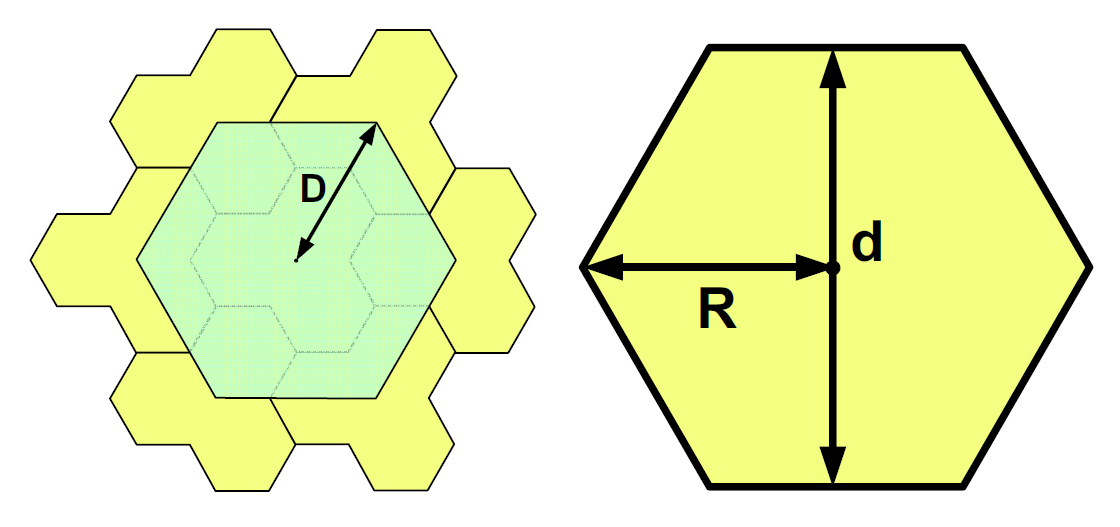
\includegraphics[width=7cm]{./bilder/systems-cluster.png}
	\end{minipage}

\subsubsection{Cochannel Interference $C/I$ \formelbuch{238}}
    \begin{minipage}{12.5cm}
        Interferenz von nächster Zelle mit gleicher Frequenz wird als Cochannel Interferenz $C/I$ angegeben.
        $$ C/I_{\text{lin}} = \frac{r^{-4}}{6d^{-4}} = \frac32 N^2 \qquad \Rightarrow \qquad 
        C/I_{\text{dB}} = 1.76 + 20 \logd N $$
        \begin{center}
            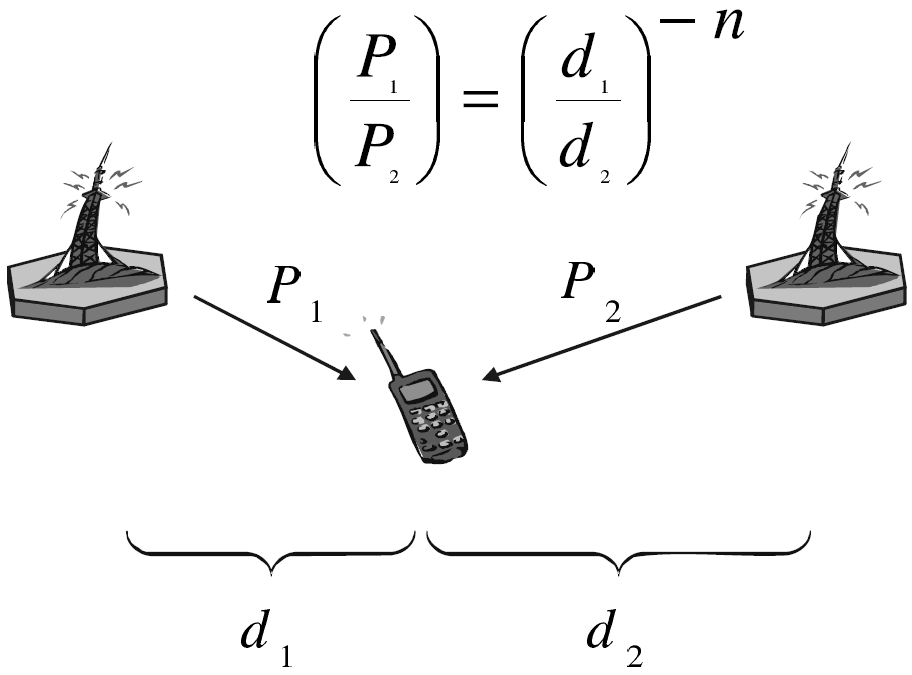
\includegraphics[width=3cm]{./bilder/systems-ci.png}                
        \end{center}
    \end{minipage}
    \begin{minipage}{6.5cm}
        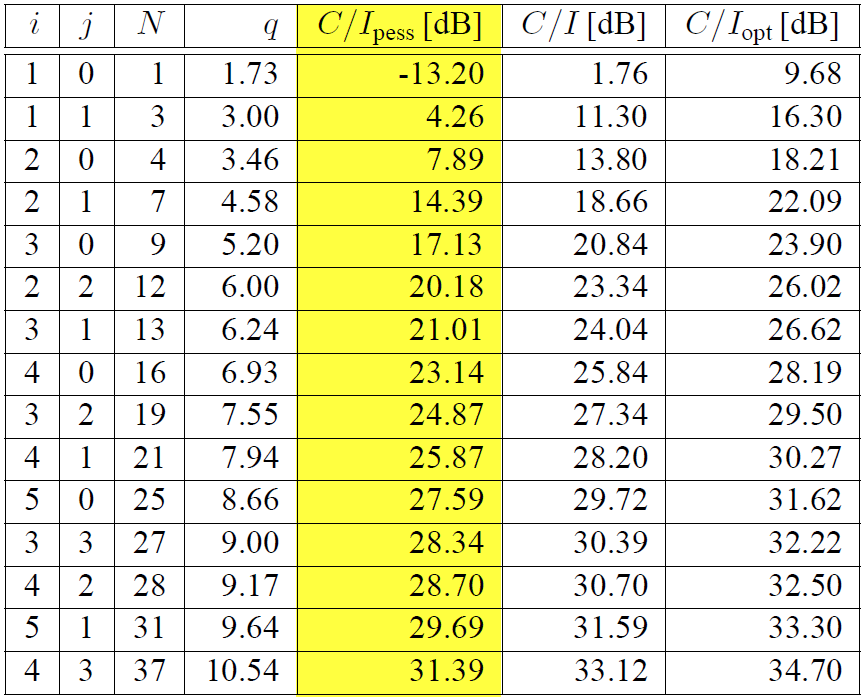
\includegraphics[width=6.5cm]{./bilder/systems-gsm-CItable.png}    
    \end{minipage}

\subsubsection{Sektorisierung \formelbuch{239}}
	Durch Sektorisierung wird die $C/I$ wird um \textbf{Faktor 3 gesteigtert}. Die Antenne wird im Zentrum der Zelle
	aufgestellt und deckt 1/3 der Zelle ab. \textcolor{green}{Vorteile:} $C/I$ verbessert $\Rightarrow$ Clustergrösse kann reduziert werden;
	\textcolor{red}{Nachteile:} Zusätzlicher Hardwareaufwand (Richtantennen, \ldots), Mehr Frequenzen benötigt, Mehr Signalisierung wegen häufigerem Kanalwechsel.

\subsection{Bündelung / Erlang (Trunking)  \formelbuch{240}}
    \begin{minipage}{12cm}
    Nebst der Einteilung in verschiedene Kanäle (FDMA) werden die Benutzer in Zeitschlitze (TDMA) gebündelt,
    um eine grössere Kapazität zu erreichen. \\
    Der Datenverkehr in Mobilfunknetzen wird in \textbf{Erlang} gemessen:
    \begin{liste}
        \item 1 Erlang $\Rightarrow$ 1 Benutzer telefoniert 100\% der Zeit
        \item 2 mE $\Rightarrow$ 1 Benutzer telefoniert 0.2 \% der Zeit
    \end{liste} 
    \vspace{0.2cm}
    Die Wahrscheinlichkeit, dass ein Benutzer blockiert wird und das Telefonat nicht ausführen kann ist gegeben durch
    \text{P(blocking)}:        
        \begin{minipage}{6cm}
            $$   \text{P(blocking)} = \frac{\frac{A^C}{C!}}{\sum_{k=0}^C\frac{A^k}{k!}} , $$            
        \end{minipage}
        \begin{minipage}{4.5cm}
            $A$: Traffic intensity, $[A] = E$ \\        
            $C$: Anzahl Kanäle, $[C] = 1$           
        \end{minipage}       
    Die nebenstehende Grafik zeigt die Blockierungswahrscheinlickeit abhängig von der Traffic Intensity und der Anzahl Kanäle. 
    \end{minipage}
    \begin{minipage}{0.3cm}
        \quad
    \end{minipage}
    \begin{minipage}{7cm}    
        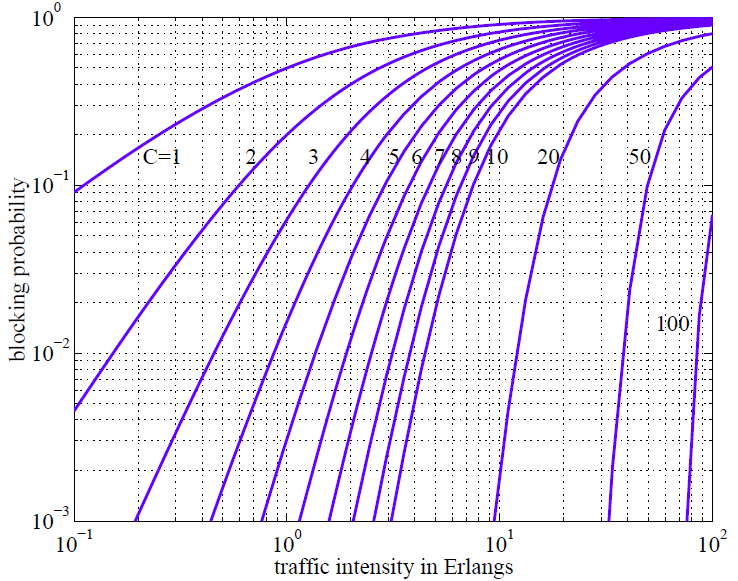
\includegraphics[width=7cm]{./bilder/systems-erlangB-graph.png}
    \end{minipage}
\newpage
\section{Multiples Access and Modulation \formelbuch{51}}
\subsection{Kanalzugriff}
	Den Kanalzugriff muss nur für Systeme mit mehreren unterschidlichen Sender bzw.
	Empfängern geregelt werden. Folgende Möglichkeiten bestehen:\\

\subsubsection{FDMA - Frequency Division Multiple Access - Frequenz-Multiplexing
\formelbuch{52}} Prinzip:\\Jeder Benutzer sendet auf einer zugewiesenen Frequenz mit einer
		definierten Bandbreite.\\
		Einsatzort:\\FM, aber auch GSM im Up-, wie auch im Downlink-Band (siehe
		Bild)\\
\subsubsection{TDMA - Time Division Multiple Access - Zeit-Multiplexing
\formelbuch{52}}

\begin{tabular}{ll}
\parbox{11cm}{
		Prinzip:\\Jeder Benutzer bekommt einen bestimmten Zeitschlitz, um in
		diesem Pakete senden zu können. Nach einer gewissen Zeit (Frame) wiederholt sich das
		ganze\\
		Einsatzort:\\zB. GSM: In einem Frame von 4.615ms hat es jeweils 8
		Teilnehmern (siehe Bild).}
    & \parbox{9cm}{
        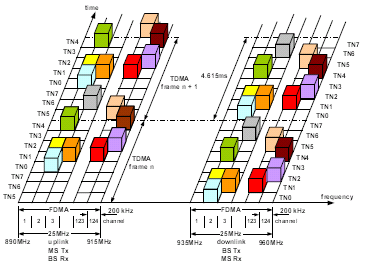
\includegraphics[width=6cm]{./bilder/modulation_TDMA.png}
        } \\
\parbox{11cm}{
		Speziell: ALOHA\\
		Für die Zuordnung der Zeitschlitze für einen neuen Teilnehmer meldet sich
		dieser zuerst bei der Basisstation. Dabei kann es zu Kollisionen mit anderen
		Teilnehmern kommen. Erneutes Melden bei der Basisstation erfolgt beim
		ALOHA-Prinzip nach einer zufällige Zeitdauer, womit die erneute
		Kollision vermieden wird.} 
	& \parbox{9cm}{
	    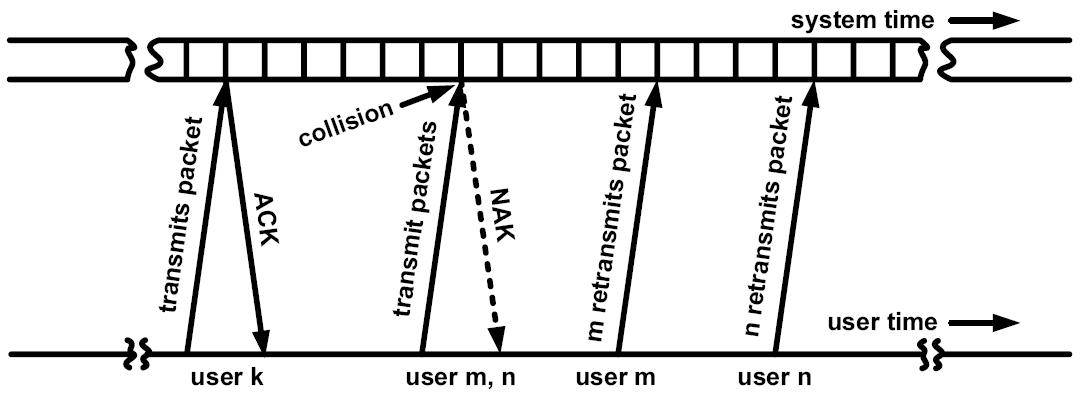
\includegraphics[width=6cm]{./bilder/modulation_aloha.png}
	    }
\end{tabular}

\subsubsection{CDMA - Code Division Multiple Access - Code Multiplexing} 
Prinzip:\\
Die Trägerfrequenzen werden mit Hilfe eines Codes zeitlich variiert. Durch eine
Korrelation mit demselben Codes kann man die richtigen Daten auch bei
Überlagerungen wieder herausfiltern. Deshalb können viele Sender bzw. Empfänger
auf demselben Frequenzband arbeiten. CDMA brauch jedoch durch das
Frequenzhopping auch mehr Bandbreite.\\
Vorteil/Nachteile:\\
+ Die Daten sind nur für die Empfänger mit den richtigen Codes sichtbar.\\
+ Sicher gegen Frequenzlöcher (da CDMA eine grosse Bandbreite benutzt).\\
+ Störsicher gegen schmalbandige Störsignale. \\
+ Bei wenigen Teilnehmern sehr gute SNR\\
+ Gut für unkoordinierte Teilnehmer (da keine Absprachen bezüglich
Zeitschlitz, Kanalfrequenz, etc. nötig sind)\\
- Schlechtes Near-Far-Verhalten
(wenn ein starker (naher) Teilnehmer einen schwachen (fernen) unterdrückt). \\
	
\textbf{Beispiel:} \\
In einem CDMA-System spreizen $K=2$ Benutzer ihre bipolaren Daten-Bits $d_k \in \{-1,+1\}$ 
synchron mit den folgenden Codes mit je $N=7$ Chips: \\
$s_1=[ -1, 1, 1, -1, -1, -1, 1 ]$, 
$s_2=[ -1, 1, 1, -1, 1, -1, -1 ]$, 
$s_3=[ 1, 1, 1, 1, -1, 1, -1 ]$, 
$s_4=[ -1, 1, -1, -1, 1, 1, -1 ]$

Der Empfänger erhält die folgende verrauschte, abgetastete Summen-Chip-Folge \\
$r=[-2, 0, -2, -2, 2, 0, -2]$ 

Um das bipolare Daten-Bit $d_1$ des Benutzer 1 zu bestimmen, kann man folgende
Formel verwenden: \\
$d_1 = sign(r\cdot s_1^T) = sign([-2, 0, -2, -2, 2, 0, -2]\cdot [ -1, 1, 1, -1, -1, -1, 1 ]^T)=sign(-2)=-1$


\subsubsection{OFDM - Orthogonal Frequency Division Multiplexing
\formelbuch{55}}

\begin{tabular}{ll}
\parbox{12cm}{
Funktioniert ähnlich wie FDMA, nur werden hier zueinander orthogonal stehende
Trägersignale verwendet, wobei jeder Träger ein Symbol (ein oder mehrere Bits)
repräsentiert. Laut Definition ist dann: \\
$  \int_0^{T_S} \sin (2\pi f_i t)\sin (2\pi f_j t) dt = 
  \left\{\begin{array}{l@{\,\,\,\,} l}
         0 , &   i\not = j, \\ 
         1 , &   i = j .   \end{array} \right.$\\
Daraus folgt, dass die bei FDMA übliche Sicherheitsabstände zwischen den Trägern
null sind. 
       } 
&
\parbox{6cm}{
    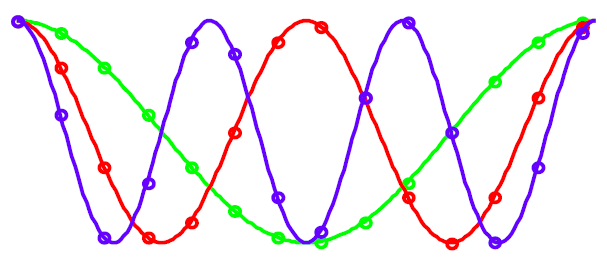
\includegraphics[width=6cm]{./bilder/modulation_OFDM-orthogonal.png}\\
    \small Orthogonalität der Träger
}       
\end{tabular}
\begin{center}
    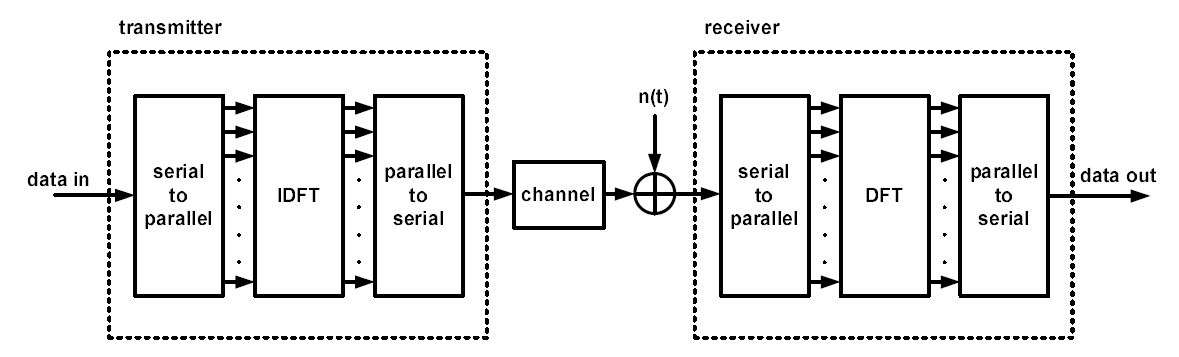
\includegraphics[width=15cm]{./bilder/modulation_OFDM-schematic.png}\\
    \small Blockschaltbild - OFDM Sender und Empfänger
\end{center}

\begin{tabular}{lll}
\parbox{4cm}{
$$\frac W{B_{\text{coh}}} \ll N_c \ll WT_{\text{coh}} $$ 
$$ T_{\text{coh}} < \dfrac{N_c}{R} = T_{\text{Subcarrier}} $$
       } 
&
\parbox{5cm}{
   $W$: Gesamtbandbreite \\
   $\dfrac{W}{N_C}$: Subcarrier Bandbreite \\
   $R$: Symbolrate (gesamtes Band)
}       
&
\parbox{9cm}{
   $N_C$: Anzahl Subcarrier bzw. Kanäle \\
   $B_{\text{coh}}$: Kohärenzbandbreite \\
   $T_{\text{coh}}$: Kohärenzzeit (Zeitinvarianz Übertragungskanal)
}       
\end{tabular}

Im Vergleich zur seriellen Übertragung ergibt sich bei der gleichen
Übertragungsrat eine viel längere
Symbolzeit, da die Daten parallel übertragen werden ergibt. Dies
ermöglicht es gegenüber Einträgerverfahren, viel weniger Bandbreite zu nutzen.
\\

Problem der \textbf{Multidimensional Interference (MDI)}:
\begin{liste}
    \item \textbf{Intersymbolic Interference (ISI)} \\
            Symbole überlappen sich im Zeitbereich (wegen Faltung mit Impulsantwort des Kanals - Laufzeit, Echo, usw.). 
			Um dies zu vermeiden wird in der Regel ein Guard Intervall $T_{Guard}$ zwischen den Symbolen eingefügt. 
			Wenn ein ISI verhindert werden soll, dann darf der Unterschied zwischen dem LOS-Ausbreitungspfad und einem 
			Nicht-LOS-Ausbreitungspfad maximal $D_{max} = c\cdot T_{Guard}$ sein.
    \item \textbf{Inter Channel Interference (ICI)} \\
            Subcarrier sind nicht mehr orthogonal. \\
\end{liste}

\begin{tabular}{lll}
	\parbox{6cm}{ 
    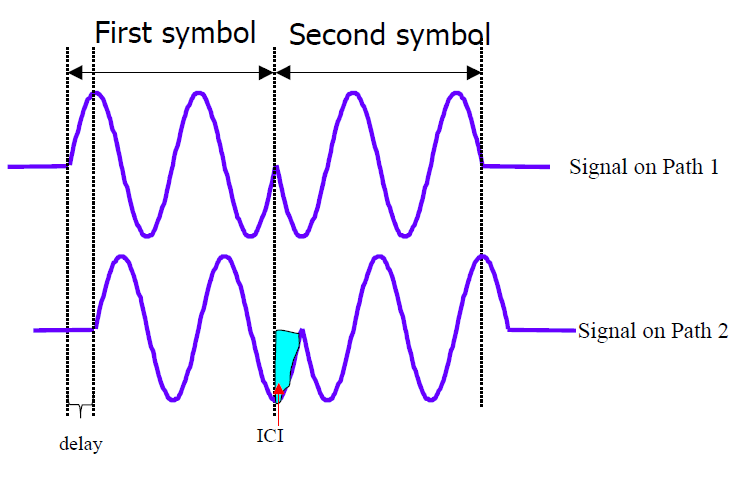
\includegraphics[width=6cm]{./bilder/modulation_OFDM-ICI.png}\\
	}    
	& \parbox{6cm}{Ein nicht-sinusförmiges Signal (Bild links) hätte mehrere/höhere
	Frequenzkomponenten zur Folge, welche in andere Subcarrier überlappen würden -
	\textbf{ICI}. Um dies zu verhindern wird das Signal mit einem sogenannten \textbf{Cyclic
	Prefix} (Bild rechts) versehen, sodass ein reines sinusförmiges Signal
	resultiert. \\	
	} &
	\parbox{6cm}{
	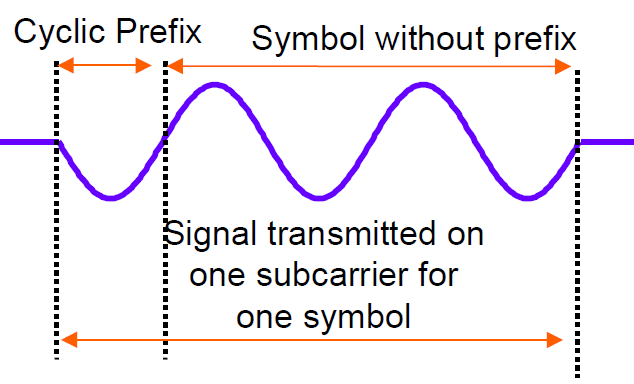
\includegraphics[width=6cm]{./bilder/modulation_OFDM-prefix.png}\\ }       
\end{tabular}


\subsection{Modulation}
Die analogen continuierlichen Modulationsarten wie AM, FM und PM werden hier
nicht behandelt. Es wird von digitalen Daten ausgegangen.

\subsubsection{Komplexes Basisband \formelbuch{57}}
Generell ist ein RF- Signal symmetrisch bezüglich des Nullpunktes
($A_1=A_{-1}$)nicht jedoch bezüglich des RF Trägers. Dies hat zur Folge, dass
das demodulierte Signal nicht mehr symetrisch zu Null ist, was bedeutet, dass
es ein komplexes Spektrum ist. $s_{RF}(t)=\Re(s_{bb}(t)e^{j2\pi f_{RF}t})$\\
\begin{tabular}{lll}
	\parbox{5cm}{
		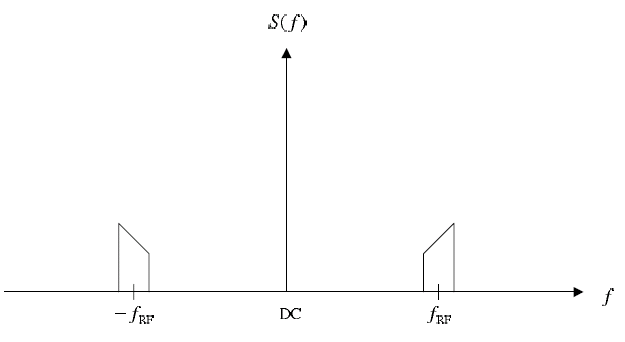
\includegraphics[width=5cm]{./bilder/modulation_RFSpektrum.png}
	}
	&$\Longrightarrow$
	&\parbox{5cm}{
		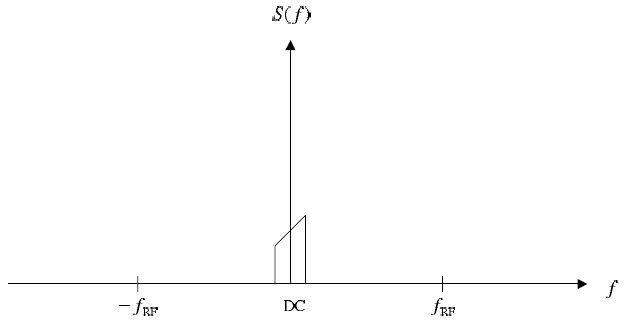
\includegraphics[width=5cm]{./bilder/modulation_BBSpektrum.png}
	}
\end{tabular}

\subsubsection{BPSK - Binary Phase Shift Keying  \formelbuch{58}}
\begin{tabular}{ll}
	\parbox{10cm}{
		\begin{tabular}{ll}
			BPSK&= 2-PAM \\
			Phase $\in \{-180^o, 0$\} &= Amplitude $\in \{-1, 1\}$
		\end{tabular}\\
		Bild rechts zeigt Amplitude und Phase des Basisbandes genau zur sampling
		time.\\
	}
	&
	\parbox{5cm}{
		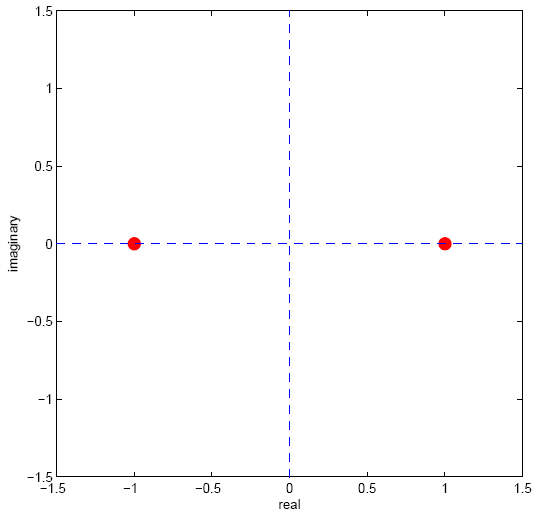
\includegraphics[width=5cm]{./bilder/modulation_constellationBPSK.png}
	}
\end{tabular}
\subsubsection{M-PAM - Pulse Amplitude Modulation \formelbuch{59}}
M kommt von M- Zuständen, welche die Amplitude annehmen kann. Dadurch können
$N=\log_2(M) [\frac{bits}{Symbol}]$ übertragen werden. Durch die Abstufung wird
die Effizienz gesteigert. Da PAM ein reelles Spektrum besitzt ist auch das
RF-Signal symmetrisch zum Träger, was jedoch die Bandbreiteneffizient stark
vermindert. Mögliche Verbesserungen:\\
\begin{liste}
	\item Zusätzlicher Imaginäranteil $\Longrightarrow$ QAM
	\item Grösseres M (Nachteil: grössere Fehlerwahrscheindlichkeit und immernoch
	symetrisch)
	\item Eliminierung des einen Frequenzbandes(z.B mit SSB)
\end{liste}

\subsubsection{M-QAM - Quadratur Amplitude Modluation \formelbuch{61}}
\begin{tabular}{ll}
\parbox{10cm}{
	Bei QAM wird die Phase und Amplidue verändert. Um eine optimale Ausnützung zu
	erhalten soll $M=2^n$ gewählt werden, wobei $n \epsilon \mathbb{N}$ und 
	$n=N=\frac{bit}{Symbol}$ist.\\
	Falls n gerade dann ergibt es ein vollständiges Viereck.\\
	Bei n ungerade ergibt sich ein Viereck ohne die Ecken.\\
	Spezialfall: 4- QAM = QPSK\\
	Das Problem für die MobKom an QAM ist, dass sich die Amplitudedämpfung sehr
	stark und relativ schnell ändern kann. Deshalb kann man keine Information als
	Amplitudenänderung senden, was dann nur noch eine Phasenverschiebung (M-PSK)
	zur Folge hat.} 
	& \parbox{8cm}{
	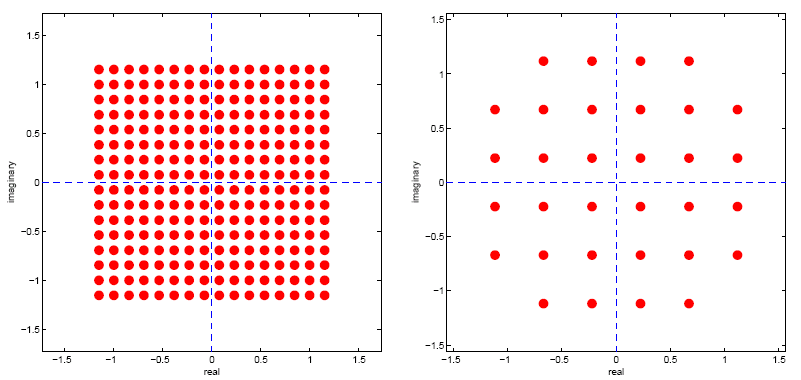
\includegraphics[width=8cm]{./bilder/modulation_constellationQAM.png}\\ 256-QAM und 32-QAM
}
\end{tabular}

\subsubsection{M-PSK - Phase Shift Keying \formelbuch{63}}
\begin{tabular}{ll}
\parbox{10cm}{
Spezielle Formen:\\
\begin{liste}
 \item Bei \textit{D}PSK kommt es nicht mehr auf die
	absolute Phase an, sondern nur noch auf den Phasensprung von Symbol zu Symbol
	(z.B. je $\frac{\pi}{4}$). So ist keine Referenz zur Nullphase nötig.
 \item \textit{$\frac{3\pi}{8}$} oder \textit{EDGE-Modulationschema} wird bei
 GSM eingesetzt. Der Vorsatz \textit{$\frac{3\pi}{8}$} bedeutet, dass zu
 einem normalen Phasensprung (hier $n \frac{\pi}{4}$ nochmals einen Offset
 von $\frac{\pi}{8}$ hinzu kommt. Dies hat zur Folge, dass die komplexe
 Amplitude nie null wird. (siehe Bild)
\end{liste}


}
&\parbox{6cm}{
    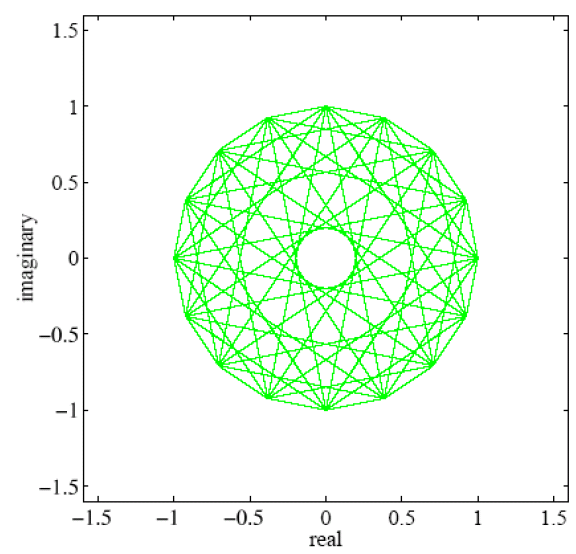
\includegraphics[width=6cm]{./bilder/modulation_constellationEDGE.png}\\
    $\frac{3 \pi}{8}$ 8-PSK

}
\end{tabular}

\subsubsection{Gray- Code \formelbuch{65}}
\begin{tabular}{ll}
	\parbox{8cm}{
		Der Vorteil des Gray Codes gegenüber der normalen binären Codierung ist, dass
		bei einem Fehler nur ein Bit falsch wird und nicht gerade alle, wie das Bild
		rechts zeigt.\\
        Bsp. aus Prüfung (12. März 2007): Vergrösserung des BER, wenn bei QPSK
        die binäre Standardcodierung statt der Gray-Codierung verwendet wird.
        
        Gray: BER = SER/2 \\
        Binär: BER = SER/2 + SER/4 \\
        Verschlechterung: $\Rightarrow 3/2$   \\ \\
        
        Für Gray-Code gilt: $\text{BER} \approx
        \dfrac{\text{SER}}{n_{\text{bits}}}$ } &\parbox{10cm}{
		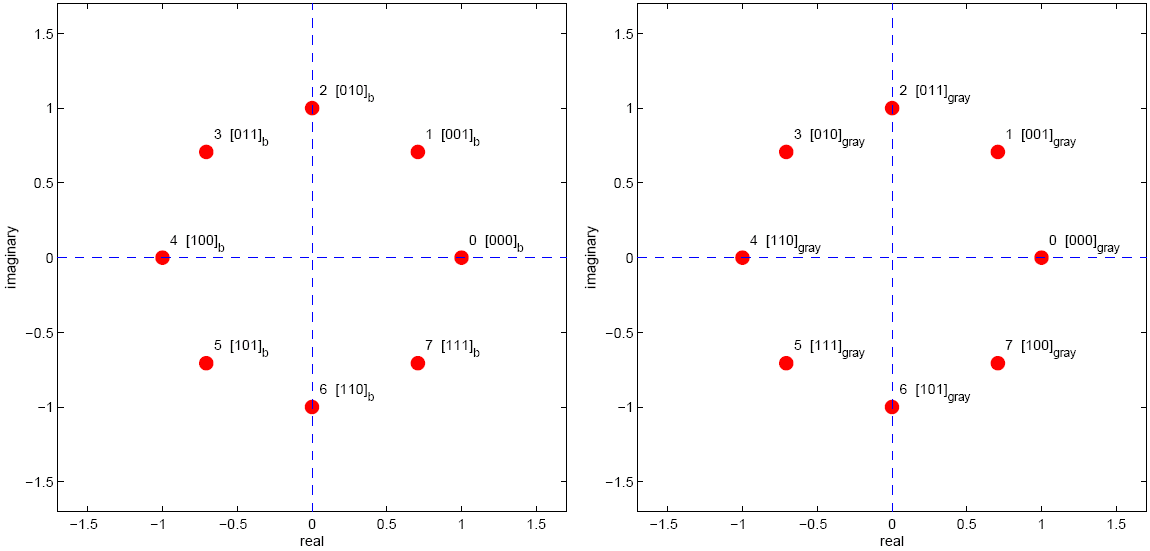
\includegraphics[width=10cm]{./bilder/modulation_PSKmitGray.png}\\
		8-PSK ohne bzw. mit Gray- Code
	}
\end{tabular}

\begin{tabular}{ll}
	\parbox{9cm}{
		\subsubsection{FSK - Frequency Shift Keying \formelbuch{65}}
		Bei FSK wird ein binäres Signal frequenz-moduliert. Das heisst,
		es switscht (hihi) zwischen zwei Frequenzen, dies wird meist mit Hilfe eines
		VCO gemacht.\\
		Kenngrösse ist der Modulations Index: \\
		$h=\dfrac{\Delta f}{f_{\text{data}}}=\dfrac{f_{\text{max}} -
		f_{\text{min}}}{f_{\text{data}}} =\dfrac{n_{\text{T-max}} -
		n_{\text{T-min}}}{n_\text{T}}$ \\ Bei einem \textbf{h von 0.5 }spricht man von
		\textbf{Minimum Shift Keying (MSK)} oder \textbf{Fast} Frequency Shift Keying
		\textbf{(FFSK)}. Trägerfrequenzen können orthogonal sein, solange der
		Modulationsindex das Minimum $h_{\text{min}}$ nicht unterschreitet. \\ $h_{\text{min}} =
		\begin{cases} 1   & \text{unkohärente Detektion} \\                                
                                0.5   & \text{kohärente - phase
                                synchron - Detektion} \end{cases}$\\
        Für unkohärente Detektion sind die beiden Träger orthogonal, wenn gilt:
        \\
        $    \Delta f = \frac{1}{T_{\text{data}}} \cdot n , \qquad n \in \lbrace
        1, 2, 3, \ldots \rbrace $
	}
	&\parbox{9cm}{
	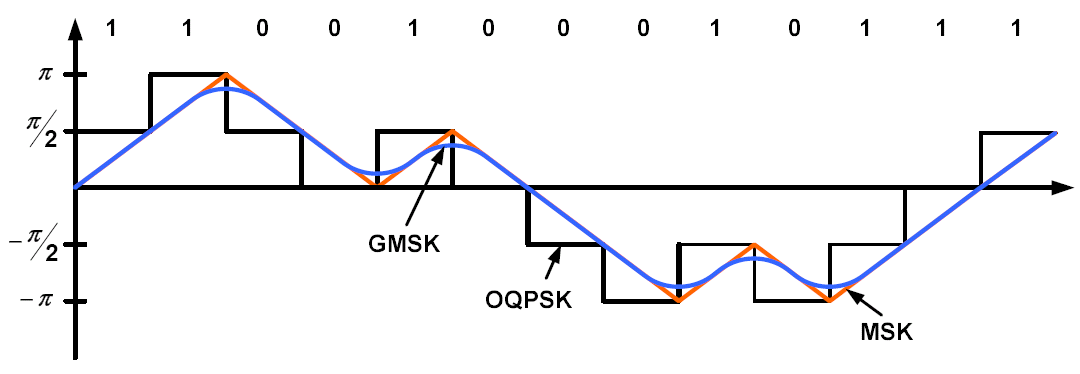
\includegraphics[width=9cm]{./bilder/modulation_phasenverschiebungGMSK_MSK.png}\\
	Phasenverschiebung des MSK bzw GMSK. }
\end{tabular}
     
        
\subsubsection{GMSK - Gaussian Minimum Shift Keying \formelbuch{67}}
Das GMSK ist ein MSK mit einem gauss'schen premodularen Filter, welches eine gauss'sche Pulsform
anstelle der sinusförmigen Pulsform erzeugt. Es besitzt eine
konstante Amplitude und eine grosse spektrale Effizient. 

Bei GSM wurde zu Beginn GMSK verwendet. Siehe Kapitel \ref{sec:gsm} - Modulation.
        

\subsubsection{OQPSK - Offset Quadratur Phase Shift Keying \formelbuch{75, 68}}
Das OQPSK ist eine Sonderform der Quadraturphasenmodulation
	
	
\subsection{Modulationskriterien}
Es gibt 3 Wege um die Fehlerwahrscheinlichkeit
herauszufinden:
\begin{liste}
	\item Austesten und messen (dauert bei kleiner Fehlerwahrscheinlichkeit so
	lange, bis ein vernünftiges Resultat erreicht wird).
	\item Simulieren (dazu ist ein gutes Model nötig, kann unter Umständen gleich
	lange dauern wie austesten).
	\item Analystisch mit Symbol- und Biterrorrate.
\end{liste}
\subsubsection{SER - Symbolfehlerrate \formelbuch{70}}
\begin{tabular}{ll}
\parbox{8cm}{
    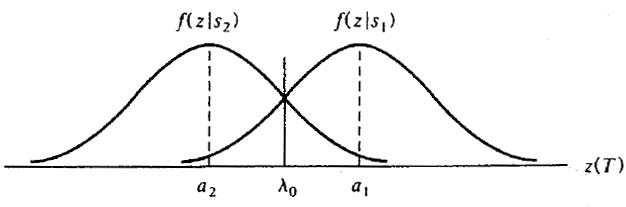
\includegraphics[width=8cm]{./bilder/modulation_AWGN.jpg}
    }
& \parbox{9cm}{
	Die Symbolfehlerrate wird unter anderem verursacht durch das thermische
	Rauschen (AWGN). Dieses hat die Energie\\ 
	$\sigma^2=\frac{N_0}{2}$ \\
	\\
	Die Fehlerwahrscheinlichkeit ist $P_E=Q(\sqrt{\frac{2 E_S}{N_0}})$ mit $a_1 =
	E_S, a_2 = -E_S$ und $\lambda_0 = 0$\\
    }
\end{tabular}

\small
\renewcommand{\arraystretch}{0.6}
% \hspace*{10mm}
\begin{tabular}[ht]{|l|l|l|l|l|}\hline
Modulation & levels/ & normalized & SER (AWGN)
           & Comments \\
scheme     & range   & amplitude  &     &          \\
\hline \hline
%&&&&\\[-3mm]
BPSK & $\pm A$& $A=1$ &
  $Q{(\sqrt{\frac{2E_s}{N_0}})}$ & \\[2mm]  \hline
%&&&&\\[-3mm]
DPSK & $\pm A$& $A=1$ &
  $2Q(\sqrt{\frac{2E_s}{N_0}})$ & coherent \\ 
  &&& $\frac{1}{2}e^{-\frac{E_s}{N_0}}$ & noncoherent\\[2mm] 
\hline
%&&&&\\[-3mm]
QPSK & $(\pm 1\pm j)A$ & $A=\frac{1}{\sqrt{2}}$&
  $ 1-\left(1-Q(\sqrt{\frac{E_s}{N_0}})\right)^2$ & coherent \\[2mm] \hline
%&&&&\\[-3mm]
DQPSK &$(\pm 1\pm j)A$ & $A=\frac{1}{\sqrt{2}}$& 
  $ 2\left(1-\left(1-Q(\sqrt{\frac{E_s}{N_0}})\right)^2\right)$ & coherent \\
&&&  $\frac{1}{2}e^{-\frac{E_s}{2N_0}}$ & noncoherent\\[2mm] \hline
%&&&&\\[-3mm]
$M$-PSK & $ \frac{1}{M}\sum_{m=1}^{M}
             A\delta\left(x- e^{j(2m-1)\frac{\pi}{M}}\right),$ & $A=1$&
  $ \leq 2Q(\sqrt{\frac{2E_s}{N_0})\sin\frac{\pi}{M}})$
  & coherent \\
& $\qquad \qquad \qquad \qquad \,\,\,\,\, m\le M$ &&& \\[2mm] \hline
%&&&&\\[-3mm]
$M$-PAM & $\pm (2m-1)A,\quad m\le M/2$ & $A=\sqrt{\frac{3}{M^2-1}}$ &
  $2\frac{M-1}{M}Q\left(\sqrt{\frac{E_s}{N_0}}\sqrt{\frac{6}{M^2-1}}\right)$ &
  \\[2mm]  \hline
%&&&&\\[-3mm]
$M$-QAM & $(\pm (2m-1)\pm j(2n-1))A,$ & $A=\sqrt{\frac{3}{2(M-1)}}$ 
  &$1-\left(1-2\frac{\sqrt{M}-1}{\sqrt{M}}Q\left(\sqrt{\frac{E_s}{N_0}}
   \sqrt{\frac{3}{M-1}}\right)\right)^2$ & \\
& $\qquad \qquad \quad m,n\le \sqrt{M}/2$ &&& \\[2mm] \hline
%&&&&\\[-3mm]
2-FSK &$\Delta f=h\cdot \frac{1}{T},\, h_{\min}=0.5$ &&
  $Q(\sqrt{\frac{E_s}{N_0}})$ 
  & orthogonal, coherent  \\
& \qquad \qquad \quad $h_{\min}=1$ &&
  $\frac{1}{2}e^{-\frac{E_s}{2N_0}}$ 
  & orthogonal, noncoherent \\[2mm] \hline
\end{tabular}
\renewcommand{\arraystretch}{1}


\subsubsection{BER - Bitfehlerrate \formelbuch{72}}
\begin{tabular}{ll}
	\parbox{10.5cm}{
	Sobald eine Informationsrate R kleiner als die Kanalkapazität C ist, sind
	fehlerfreie Übertragungen möglich.\\
	$C= W \log_2 ( 1+\frac{S}{N}) > R$\\
	Wobei W die Bandbreite des Kanals, N die Rauschenergie $N=N_0 W$ und S die
	Signalenergie ist.
	Die Grenze ist bei $C=R \Longrightarrow E_b C$ $E_b$ ist die Bitenergie\\

	$\Longrightarrow \frac{C}{W}= \log_2(1+\frac{E_b C}{N_0 W})$\\ 

	
	\subsubsection{Spektrale Effizient \formelbuch{75}}
	Heisst wieviel Bandbreite pro Datenrate gebraucht wird.
	Die Effizient beinhaltet zwei Kriterien:
	\begin{enumerate}
	\item Wieviele Bits können in einer gegeben Bandbreite übertragen werden. Wenn
	man die Begrenzung durch die SNR beliebig erweitern indem man die Bits/Symbol
	erhöht.
	\item Wieviel das Spektrum die Nachbarn überlagert. Je nach Modulation gibts
	einen breiten Mainlobe mit schwachen Sidelobes oder umgekehrt.
    \end{enumerate}
  
    \subsubsection{Raised-Cosine-Filter \formelbuch{63}}
    $h(t) = \frac{\sin\left((t/T)\pi\right)}{(t/T)\pi}\cdot
        \frac{\cos\left(\rho(t/T)\pi\right)}{1-4\rho^2(t/T)^2}$\\
   
    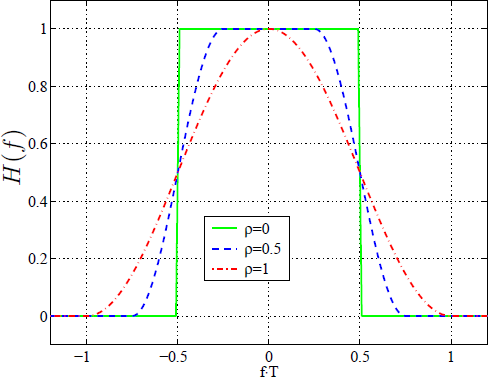
\includegraphics[width=5cm]{./bilder/modulation_raised_cosine_frequency.png}
    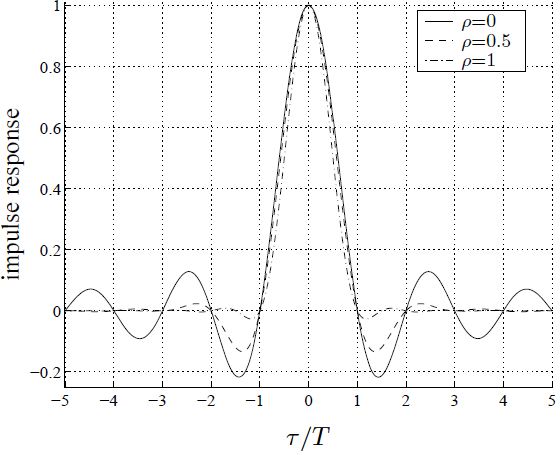
\includegraphics[width=5cm]{./bilder/modulation_raised_cosine_time.png} 
    
    Das \textbf{Root-Raised-Cosine-Filter} entspricht der Wurzel des
    Raised-Cosine-Filters und wird angewendet, wenn die Charakteristik 
    des Raised-Cosine-Filters auf Sender und Empfänger
    gleichmässig verteilt werden soll.
    } &\parbox{7cm}{
	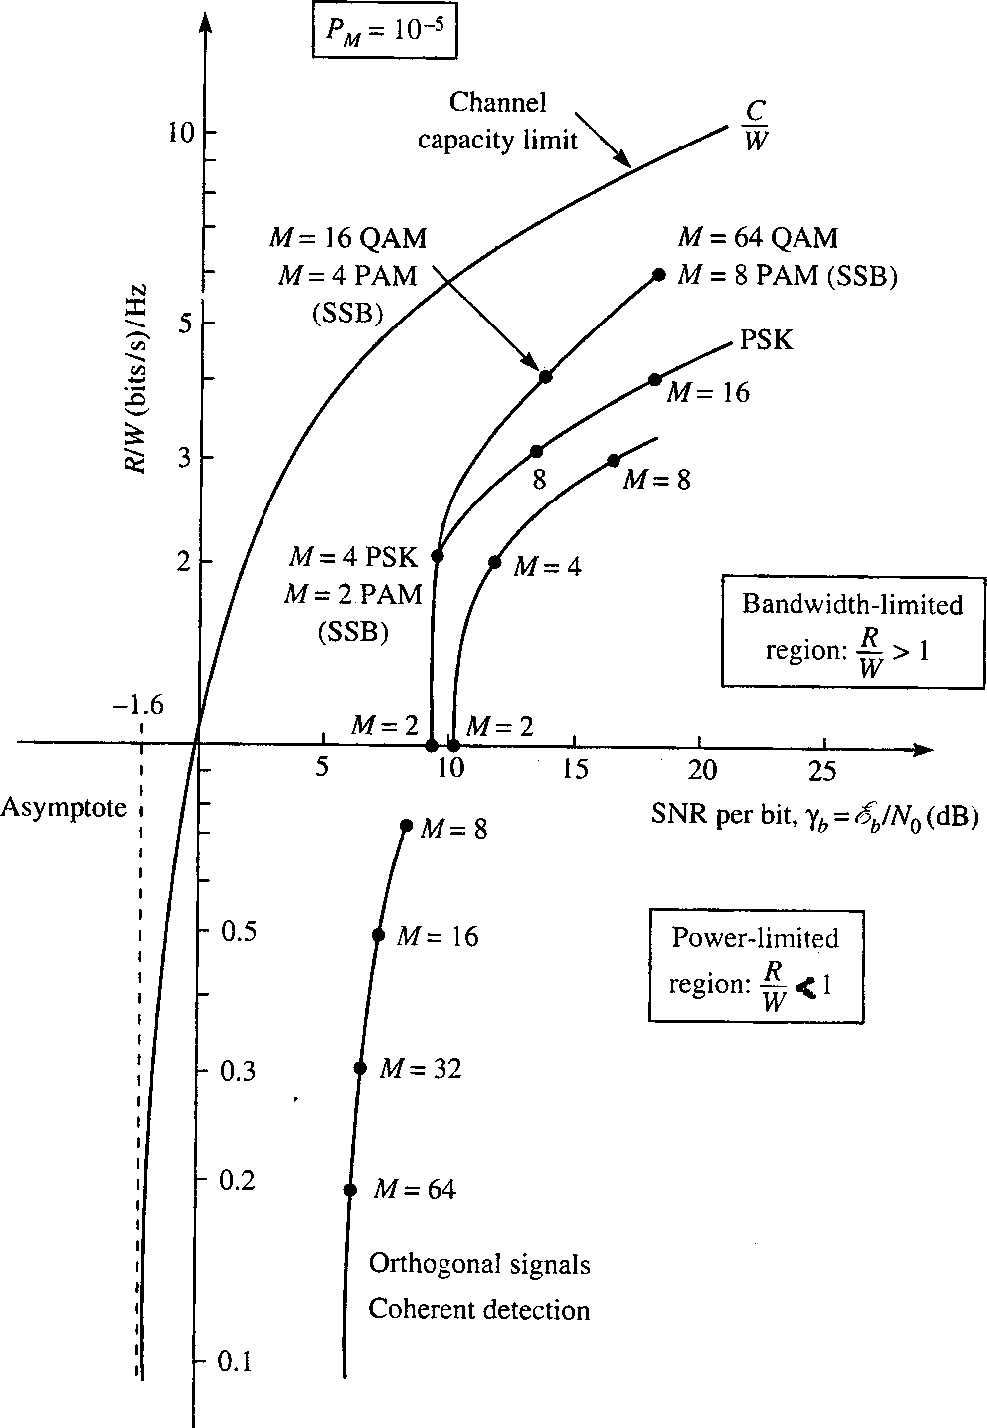
\includegraphics[width=7cm]{./bilder/modulation_SER.png}\\
	Übersicht einzelner Modulationen mit einer SER von $10^{-5}$
	}
\end{tabular}

\section{Information Theoretical}

\section{RFID - Radio Frequency IDentification}
Die ursprünglich Idee war dass RFID den Barcode ablösen sollte, doch der heutige Anwendungsbereich ist bereits schon viel breiter.
Reader $\rightarrow$ Tag: Downlink \\
Tag $\rightarrow$ Reader: Uplink

\begin{tabular}[h]{c c}

\parbox{8cm}{
    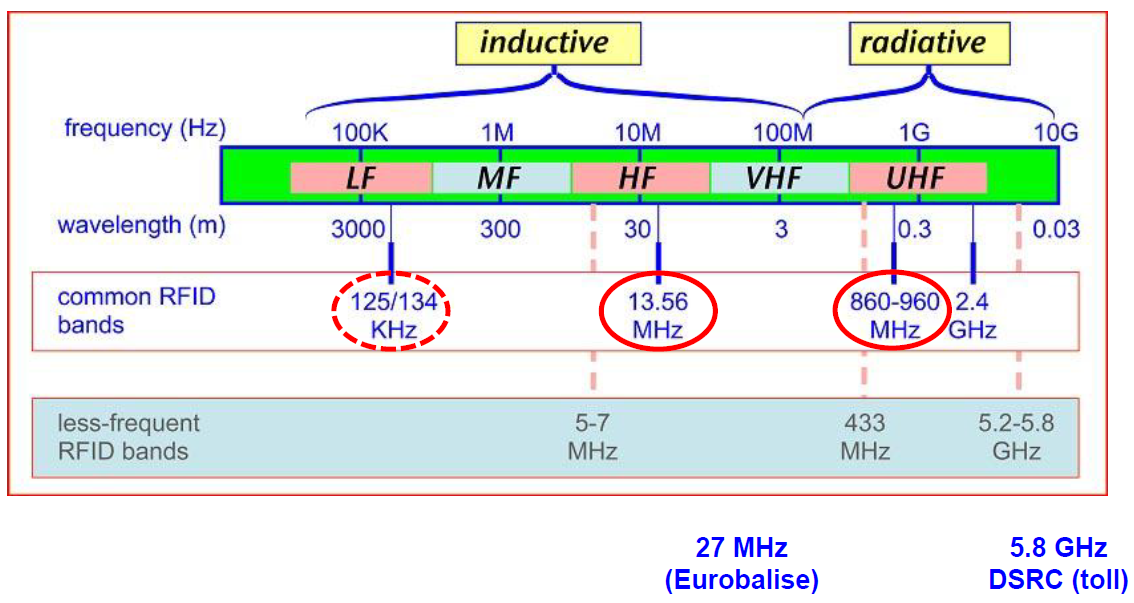
\includegraphics[width=8cm]{./bilder/RFIDFrequenzen.png} } 
&

\parbox{8cm}{
    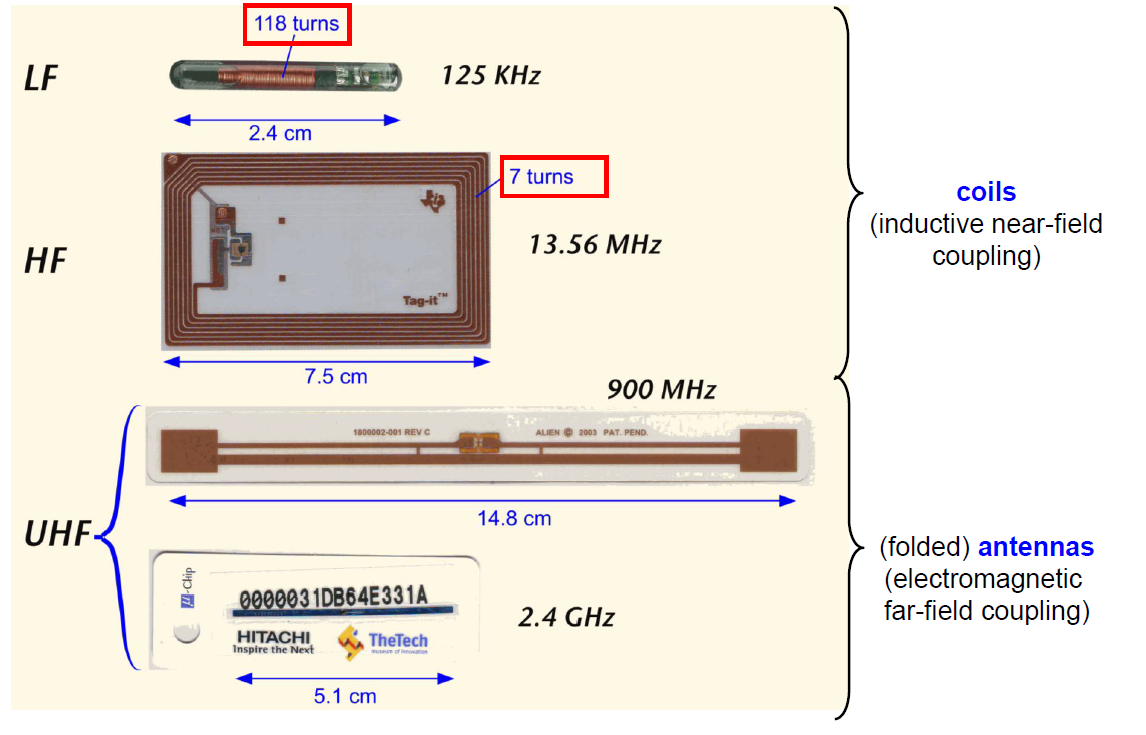
\includegraphics[width=8cm]{./bilder/RFIDTags.png} } \\
\end{tabular}
\subsection{Aktiv vs. Passiv}
	\begin{itemize}
		\item Passiv: Es sendet und empfängt gleichzeitig, Frequenzen müssen leicht verschoben sein
		\item Semi-Passiv: Es kann nur antworten, wenn es angestrahlt wird. Es hat Batterie für Tag Power aber nicht für Radioteil. 
		\item Aktiv: Es kann antworten auch wenn es nicht angestrahlt wird. Es hat Batterie für Tag und Radio. 
	\end{itemize}
\subsection{Antikollisionsprotokolle}
	\begin{tabular}{ll}
		\parbox{9cm}{
			\begin{itemize}
				 \item Deterministisches Antikollisionsprotokoll: Baumsuche anhand von uniqueID (und Maske). Leserate: 10-30 Tags/s
				 
				 \item Probabilistisches Antikollisionsprotokoll: Modifiziertes ALOHA-Protokoll (mit Random Nr). Leserate. 100-500 Tags/s
			\end{itemize}
		}	
		& \parbox{9cm}{
			\fbox{ 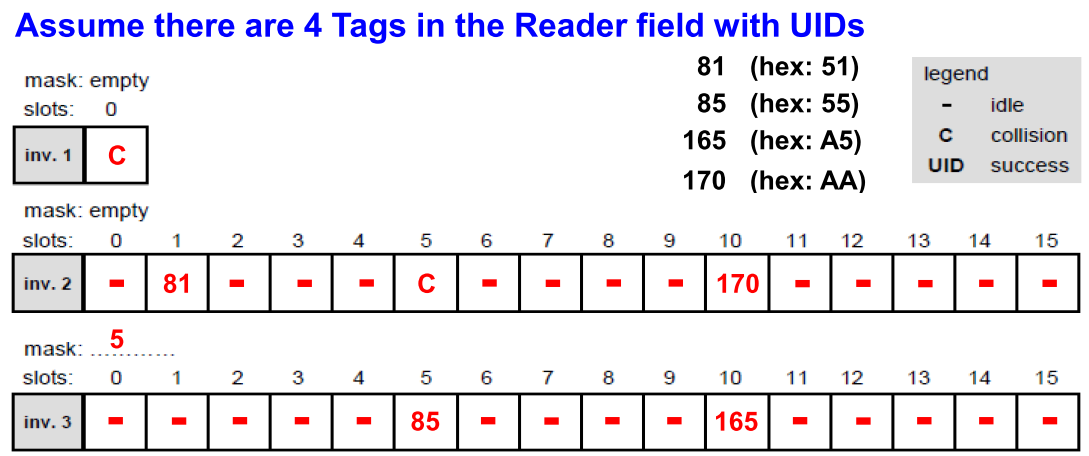
\includegraphics[width=9cm]{./bilder/rfid-anticollision.png}}\\ Bsp. Deterministic Anticollision
		}
	\end{tabular}
	
	Tags sollten einen gewissen Abstand voneinander haben um zu vermeiden dass sie sich gegenseitig stören (Schwingkreisverstimmung).

\subsection{Standards}
	\begin{itemize}
		\item LF
			\begin{itemize}
				\item ISO/IEC 11784/5 and extension 14223 identification of animals
			\end{itemize} 
		\item HF
			\begin{itemize}
				\item ISO/IEC 14443	Identification Cards – Proximity Cards (2001) 
					\begin{itemize}
						\item 2 completely different data transmission types (A and B), incompatible (Reader must support both)
						\item range up to 10 cm, data rate 106 kb/s, 13.56 MHz, inductive coupling
						\item typical application: e-ticketing, micro-payment (e.g. Metro-tickets)
					\end{itemize}
				\item ISO/IEC 15693	Identification Cards – Vicinity Cards (2001/2009)
					\begin{itemize}
						\item range up to 1m, data rate 26 kb/s, ISO/IEC 18000-3 mode 1, 13.56 MHz, inductive coupling
						\item Moving tag reading rate: 125 Tags/s (max. 1 Tag in Reader field), otherwise 10-30 Tags/s
						\item Minimum exposure time in Reader field access approx. 8 ms
						\item Deterministic anticollision-protocol (anhand von uniqueID und Maske)
						\item Memory: max. 8kByte (either 256 blocks x 256 bits or 2048 blocks x 32 bits with protocol extension)
						\item Tags are uniquely identified by a 64 bits unique identifier (UID)
						\item typical application: Access, Ski-Pass, item management
					\end{itemize}
				\item ISO/IEC 18000-3 mode 3(item management standard)
					\begin{itemize}
						\item range up to 1m, less used HF-version of EPC UHF Gen2, typically 53 kb/s (ETSI), 13.56 MHz, inductive coupling
						\item slotted ALOHA based anticollision algorithm allows up to 150 Tags/s
					\end{itemize}
						
			\end{itemize}
		\item UHF
			\begin{itemize}
				\item ISO/IEC 18000-6C item management standard - EPC (Electronic Product Code) Gen2 UHF
					\begin{itemize}
						\item Tags can be used worldwide in the 860-960 MHz band, radio coupling
						\item range up to 16m, max. ERP = 2.0 W (i.e. EIRP = 3.28 W), datarate ETSI 100kb/s (FCC: 200kb/s)
						\item slotted ALOHA based anticollision algorithm allows up to 400 Tags/s
						\item EPC is only an ID (96-496 bits), the information is stored on the network
					\end{itemize}
			\end{itemize}
		\item NFC-Interface and Protocol Standards
			\begin{itemize}
				\item NFCIP-2 (ECMA-352 / ISO-21481) 
				\item NFCIP-1 (ECMA-340 / ISO-18092) 
			\end{itemize}
	\end{itemize}	
	
\subsection{RFID LF}
	\begin{itemize}
		\item Frequenz: Um 125-134kHz
		\item Induktive Kopplung (Spulen als Empfänger) - inductive near-field coupling 
		\item Tiefe Frequenz $\rightarrow$ 100-1000 Windungen
		\item Flüssigkeiten haben nur einen geringen, Metalle haben einen grossen Störeinfluss
		\item Downlink: ASK Modulation
		\item Uplink: Load Modulation (durch kurzschliessen der Tag-Antenne wird Gegenfeld erzeugt welches Feld des Readers schwächt)
		\item Anticollision: ALOHA
		\item Typische Anwendung: Tier-Identifikation
	\end{itemize}
	
\subsection{RFID HF}
	\begin{itemize}
		\item Frequenz: 5MHz - 100MHz
		\item Typischerweise 13.56MHz (90\% aller RFID Applikationen arbeiten mit dieser Frequenz)
		\item Induktive Kopplung (Spulen als Empfänger) - inductive near-field coupling (-60dB/decade)
		\item Downlink: ASK Modulation
		\item Uplink: Load Modulation
		\item Anticollision: ALOHA
		\item Reader Talks first
		\item Hohe Frequenz $\rightarrow$ 3-10 Windungen
		\item Spulengrösse $\rightarrow$ Leseabstand = Spulendurchmesser von Reader Antenne
	\end{itemize}
\subsubsection{Modulation bei induktiver Kopplung}
	\begin{itemize}
		\item Downlink: ASK Modulation, Nicht zu viele Nullen senden, sonst hat Tag zu wenig Power. Je höher Modulationstiefe, umso weniger Energie. 
		\item Uplink: Lastmodulation, Manchester coded, Tag schliesst Antenne kurz, wird auf Hauptträger draufmoduliert (mit Subträger) $\rightarrow$
		Der Reader kann nicht auf der gleichen Frequenz ein kontinuerliches Signal senden und gleichzeitig empfangen, deshalb wir mit hilfe der Subträger
		das Spektrum verschoben (siehe Bild unten). Es kann nur 1 oder 2 Subträger verwendet werden (bei 2 Subträgerfrequenzen spricht man von FSK-Modulation).
	\end{itemize}
	
	\begin{minipage}{12cm}
		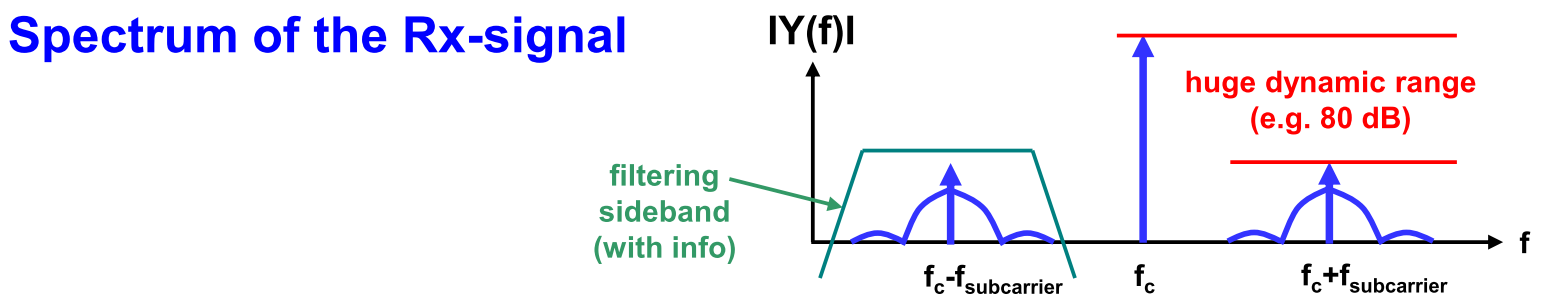
\includegraphics[width=12cm]{./bilder/rfid-spectrum.png} 
	\end{minipage}
	
	Beim Design induktiver Reader- und Tag-Antennen wird die Güte Q so gewählt, dass sich ein Kompromiss zwischen lange Distanz (hohe Spannungsspitzen) 
	und guter Träger-Subträger-Trennung ergibt.
	

\subsection{RFID UHF}
	\begin{itemize}
		\item Frequenz:	100 MHz - 10 GHz
		\item Typische Frequenzen sind 860-960 MHz oder 2.4GHz
		\item Elektromagnetische Kopplung (Antenne zum Empfangen) - electromagnetic far-field coupling
		\item Flüssigkeiten absorbieren die Strahlung und Metall hat einen grossen Einfluss
		\item Leseabstand bei passiven Tags bis zu 5-8 m (semi-passive bis 15m, aktive bis 100m)
		
	\end{itemize}

\subsubsection{Modulation bei elektromagnetischer Kopplung}
	\begin{itemize}
		\item Downlink: ASK Modulation, Nicht zu viele Nullen senden, sonst hat Tag zu wenig Power. Je höher Modulationstiefe, umso weniger Energie. 
		\item Uplink: Backscatter Modulation, Tag schliesst Antenne kurz, wird auf Hauptträger draufmoduliert (mit Miller-Modulierter Subträger)
	\end{itemize}

	\begin{minipage}{12cm}
		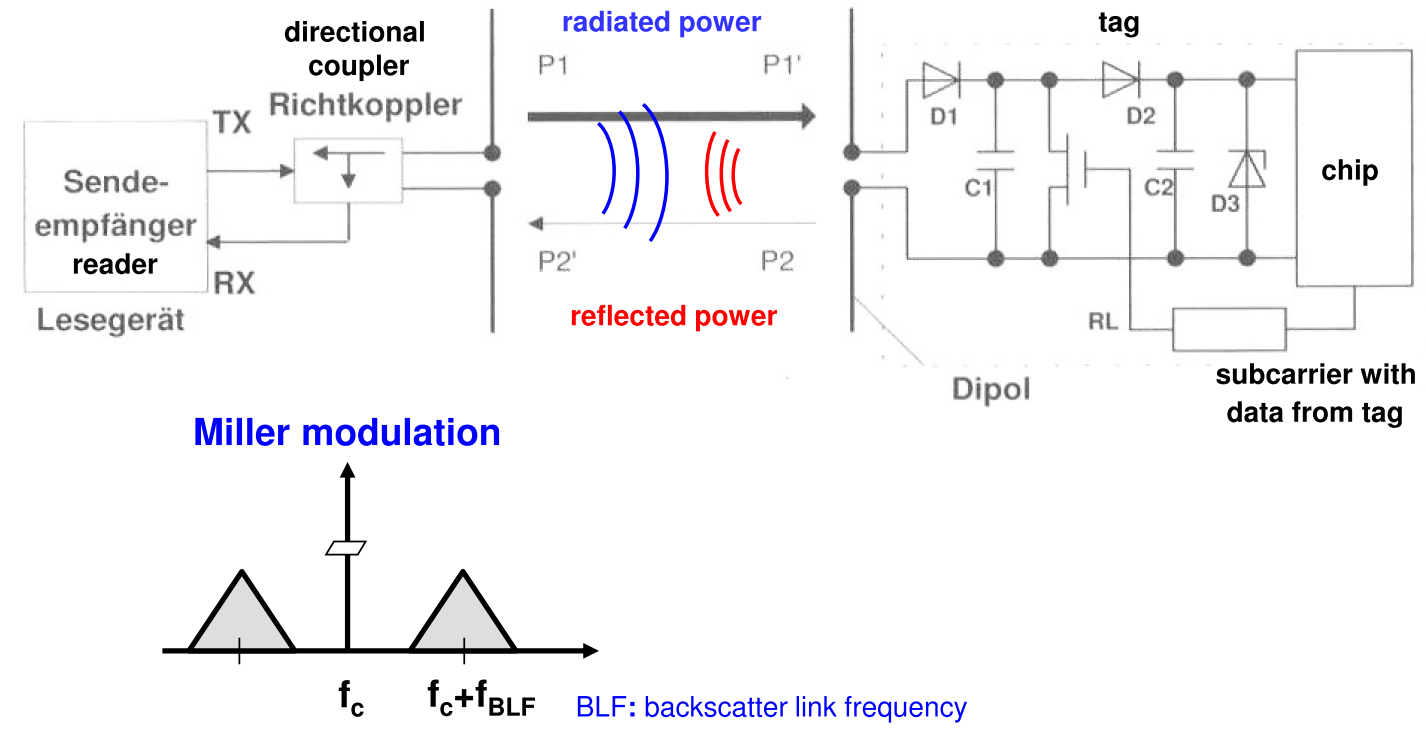
\includegraphics[width=12cm]{./bilder/rfid-millermod.png} 
	\end{minipage}
	
\subsection{NFC - Near Field Communication}
	
	\begin{minipage}{10cm}
		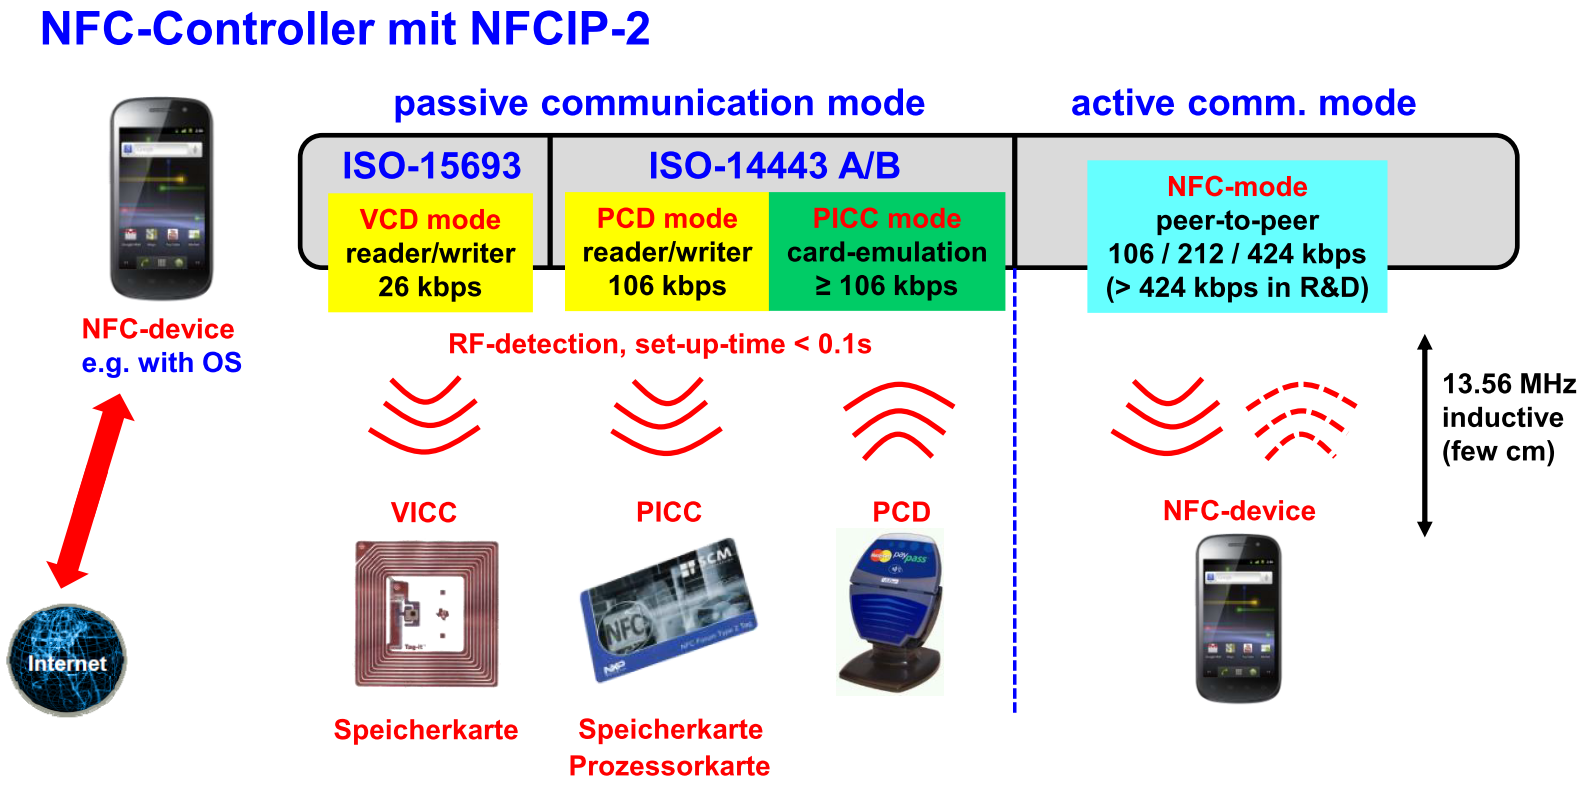
\includegraphics[width=10cm]{./bilder/rfid-nfc.png} 
	\end{minipage}
			
	NFC wird heute häufig als Synonym für RFID verwendet. NFC ist aber ein \textbf{Standard} welcher physikalisch ein RFID-Interface benutzt. 
	NFC ist beides = Auf der physikalischen Ebene RFID und auf protokol Ebene etwas Spezielles.
	\begin{itemize}
		\item Active Mode - Peer-to-Peer mode, ASK-modulation in both directions, max. 424 kb/s, range up to 20cm
		\item Passive Mode - Reader Emulation, ISO 14443 and 15693 Tags can be read
		\item Passive Mode - Card Emulation, market driver (wallet-app)
	\end{itemize}
	
	
\section{Bluetooth BR/EDR (Basic Rate/Enhanced Data Rate)}
\subsection{Summary}
\begin{itemize}
	\item Applications: cable replacement, ad-hoc networking, WPAN 
	\item Standard: Industry standard of Bluetooth SIG (Special Interest Group): http://www.bluetooth.org 
	\begin{itemize}
		\item BT Spec V1.1:  Basis for 1. Basic-Rate-(BR-) products, $R_{max} = 0.7$ Mbps, IEEE 802.15.1-2002 
		\item BT Spec V1.2:  Adaptive FH  
		\item BT Spec V2.0:  Enhanced Data Rate (EDR), $R_{max}  = 2.1$ Mbps 
		\item BT Spec V2.1:  Secure Simple Pairing 
		\item BT Spec V3.0:  Alternative 802.11 MAC PHY (AMP), high speed (HS-) version, $\leq 24$ Mbps 
		\item BT Spec V4.0:  released 2010, BR/EDR and HS-option, and Bluetooth Low Energy 
	\end{itemize}
	\item Frequency Band: 2.4 GHz ISM-band, 79 channels with 1 MHz carrier spacing between 2402-2480 MHz
	\item Multiple Access
	\begin{itemize} 
		\item FHSS for interference mitigation (1600 hops/s, 625 us time slots, Time-Division-Duplexing) 
		\item FH-CDMA for piconet separation 
		\item Adaptive FH (AFH) to support coexistence with other systems, e.g. WLAN  
	\end{itemize}
	\item Modulation
	\begin{itemize}
		\item BR: GFSK, gross bit rate 1 Mbps  (Bluetooth symbol period is 1us)
		\item EDR: $\pi/4$-DQPSK or 8DPSK, gross bit rate 2 Mbps or 3 Mbps 
	\end{itemize}
	\item Error Control: CRC, FEC with $R=1/3$, $2/3$ or $R=1$ (no FEC), fast ARQ 
	\item Packet Length: 1-, 3- and 5-slot-packets (no FH during transmission), max. payload 1021 Bytes 
	\item Data Rates
	\begin{itemize}
		\item asynchronous:  $R \leq 531$ kbps (1-slot-packets only), $R \leq 1.3$ Mbps (symmetric), $R \leq 2.1$ Mbps (asymmetric) 
		\item synchronous:   $R = 64$ kbps (BR, voice), $R \leq 864$ kbps (EDR, high quality audio streaming) 
	\end{itemize}
	\item Power Classes:  class 1:  $P_{max} = 100$ mW (20 dBm), class 2:  $P_{max}  = 2.5$ mW (4 dBm), class 3:  $P_{max} = 1$ mW (0 dBm) 
	\item Sensitivity: specified -70 dBm, most devices achieve -80 dBm or better 
	\item Radio Range: indoor: 10 m with 1 mW power and 30 m with 100 mW 
	\item Architecture: 
	\begin{itemize}
		\item a Bluetooth-device can be master or slave 
		\item all Bluetooth-devices have a worldwide unique 48 bit Bluetooth Device Address (BD-Addr) 
		\item piconet:   1 master and up 7 slaves, synchronized to the master’s hopping sequence \\ 
		low power modes : park, hold or sniff state \\
		point-to-point and (asynchronous) broadcast communication 
		\item scatternet:  interconnected piconets (rarely used), a slave can participate in 2 piconets 
	\end{itemize}
	\item Protocol Stack: Core protocols like radio, baseband, etc. and Host Controller Interface (HCI) \\
	Profiles (e.g. Serial Port Profile, SPP) to provide interoperable services  
	and to adapt Bluetooth e.g. to audio-, TCP/IP- or AT-modem-applications 
	\item Security
	\begin{itemize}
		\item secure simple pairing based on public key protocols 
		\item challenge-response-authentication 
		\item stream ciperhing with 128 bit cipher key (SAFER+ algorithm) 
	\end{itemize}
	\item Some Disadvantages
	\begin{itemize}
		\item inquiry scan can last 5-10s 
		\item connecting time after pairing $\leq 30$ms
		\item current consumption and SW-stack too large for many low rate wireless devices/sensors \\
		\textit{typical current consumption of a bluetooth module with some profiles: 25 mA $@$3.0V for Tx (Peak $< 30$mA)}
		\item low cost for very high volumes only (some million chips / devices)  \\
		\textit{module solution with profiles costs 10-15 CHF $@$ 100k devices per year}
	\end{itemize}
\end{itemize}

\subsection{Piconet}
	\begin{tabular}{ll}
		\parbox{14cm}{
			A Bluetooth piconet is an ad-hoc network consisting of 1 master and 1 to 7 slaves 
			whereby all devices of the piconet have the same hopping sequence (and share the 
			same 1 MHz channel). The hopping sequence is derived from the master’s clock  
			and the master's Bluetooth device address BD-ADDR. 

			A number of independent piconets may exist in close proximity. Each piconet has a 
			different physical channel (that is a different master device and an independent timing 
			and hopping sequence.) 
			
			A Bluetooth device can never be a master of more than one piconet, since in BR/EDR the piconet
			is defined by synchronization to the master's Bluetooth clock. However, a Bluetooth device 
			may be a slave in many independent piconets. It does this on a time-division multiplexing basis.
			
			Two Bluetooth slaves can only communicate with each other via the Bluetooth master. The Bluetooth
			piconet is a star or point-to-multipoint network.
			
			When a master wants to connect to a slave with an unknown Bluetooth device address, then the piconet 
			connection procedure consists of
			\begin{enumerate}
				\item the inquiry procedure and
				\item the paging procedure.
			\end{enumerate}
			
			The connection procedure can last 5-10s.
		}	
		& \parbox{4cm}{
			\fbox{ 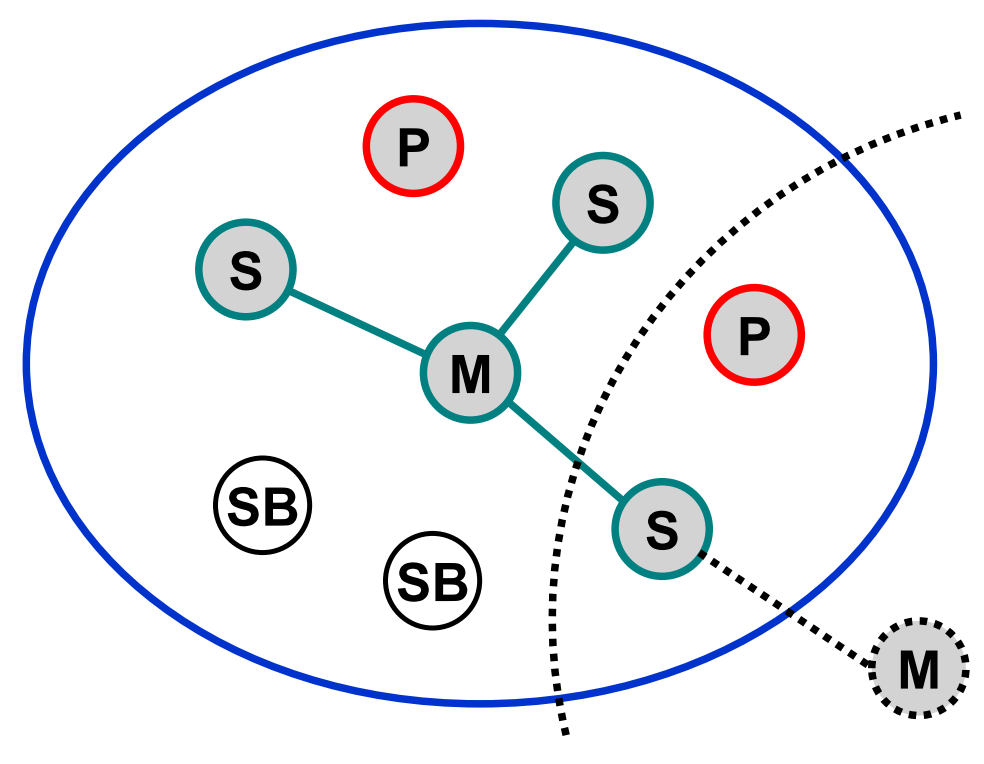
\includegraphics[width=4cm]{./bilder/bt-piconet.png}} \\ Piconet and Scatternet }
	\end{tabular}

\subsection{AFH - Adaptive Frequency Hopping}
	Adapted piconet physical channels can be used for connected devices that have AFH enabled. There are 
	two distinctions between basic and adapted piconet physical channels. The first is the same channel 
	mechanism that makes the slave frequency the same as the preceding master transmission. The second aspect 
	is that the adapted piconet physical channel may be based on less than the full 79 frequencies of the 
	basic piconet physical channel.
	
	AFH is used to improve resistance to radio frequency interference by avoiding the use of crowded frequencies
	(e.g. used by WLANs) in the hopping sequence.

\subsection{Packet transmission}
	In an EDR-packet there is a small guard time and synchronization sequence before payload. This is 
	a field used for physical layer change of modulation scheme (GFSK for the packet header and 4- or 8-PSK 
	for the payload). The packet header is GFSK-modulated in order that all Bluetooth devices can decode it.
	
	During the transmission of a multi-slot packet (e.g. 3 slots) the frequency f(k) of the master doesn't hop. When 
	the transmission is terminated, the frequency of the master hops to the next slot (e.g. f(k+3)). If there is a  
	collision in a slot during the transmission of a multi-slot packet, then the whole packet is destroyed. \\
	
	Bluetooth knows the following types of logical links:
	\begin{itemize}
		\item Synchronous Connection-Oriented \textbf{(SCO)} logical transport, point-to-point logical transport,  
		where there is no repetition of lost packets, but there are reserved slots at regular intervals 
		for maintaining the synchronous transport (e.g. for voice). 
		\item Extended Synchronous Connection-Oriented \textbf{(eSCO)} logical transport, where a repetition is possible 
		within a certain retransmission window right after the reserved slots.
		\item Asynchronous Connection-Oriented \textbf{(ACL)} logical transport, 
		\item Active Slave Broadcast \textbf{(ASB)} logical transport, used by master to communicate with active slaves
		\item Parked Slave Broadcast \textbf{(PSB)} logical transport, used by master to communicate with parked slaves
	\end{itemize}
	
	\begin{tabular}{ll}
		\parbox{9cm}{
			\fbox{ 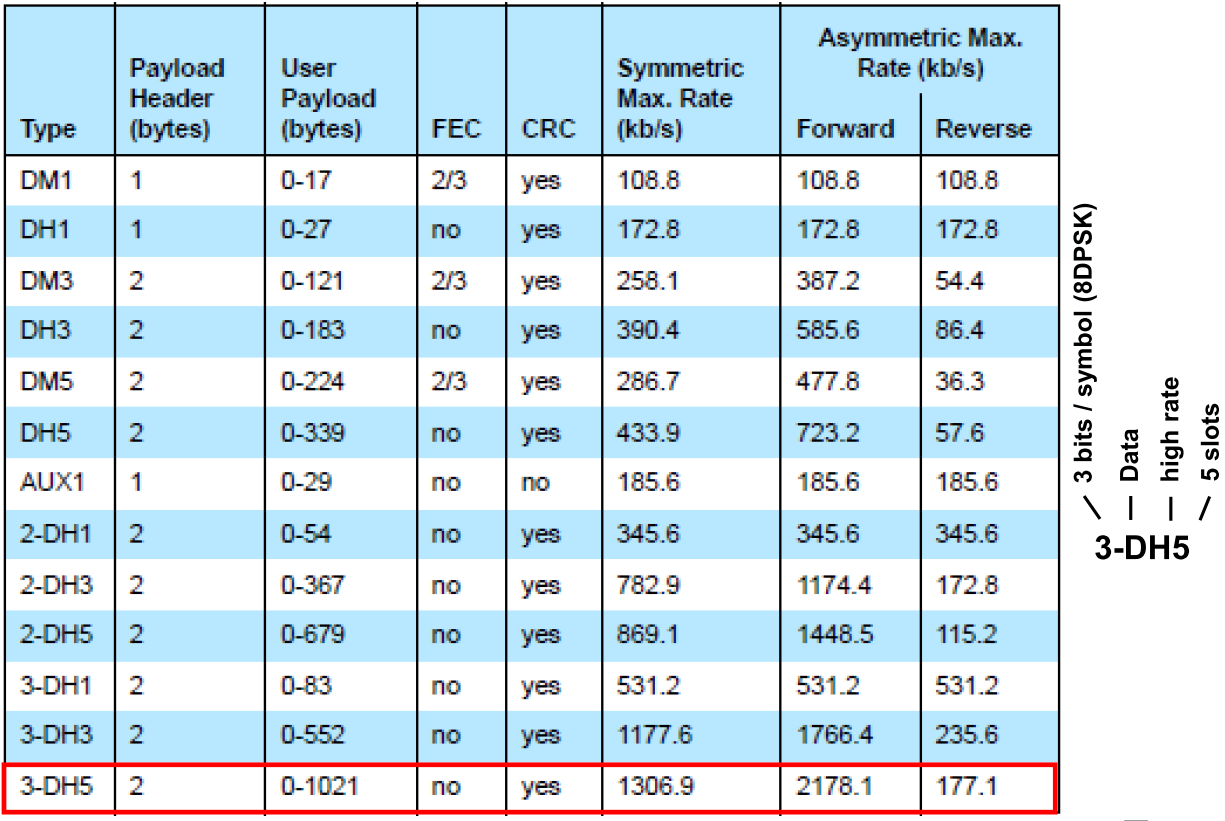
\includegraphics[width=8.5cm]{./bilder/bt-acl.png}} \\ ACL Packets 
		}	
		& \parbox{9cm}{
			\fbox{ 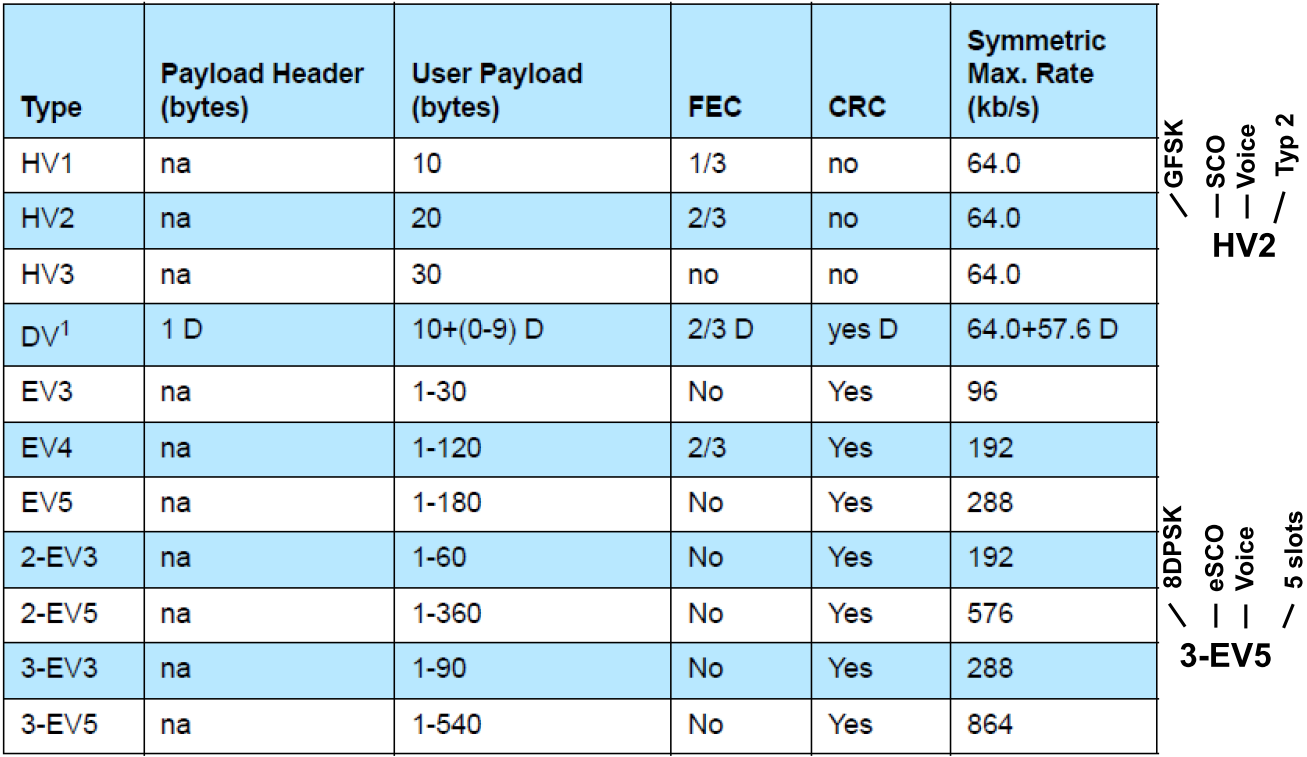
\includegraphics[width=8.5cm]{./bilder/bt-sco.png}} \\ Synchronous Packets 
		}
	\end{tabular}	\\

	The packets are transmitted in the first “part” of the time slots. The master sends always 
	in even slots. \\
	
	\begin{minipage}{16cm}
		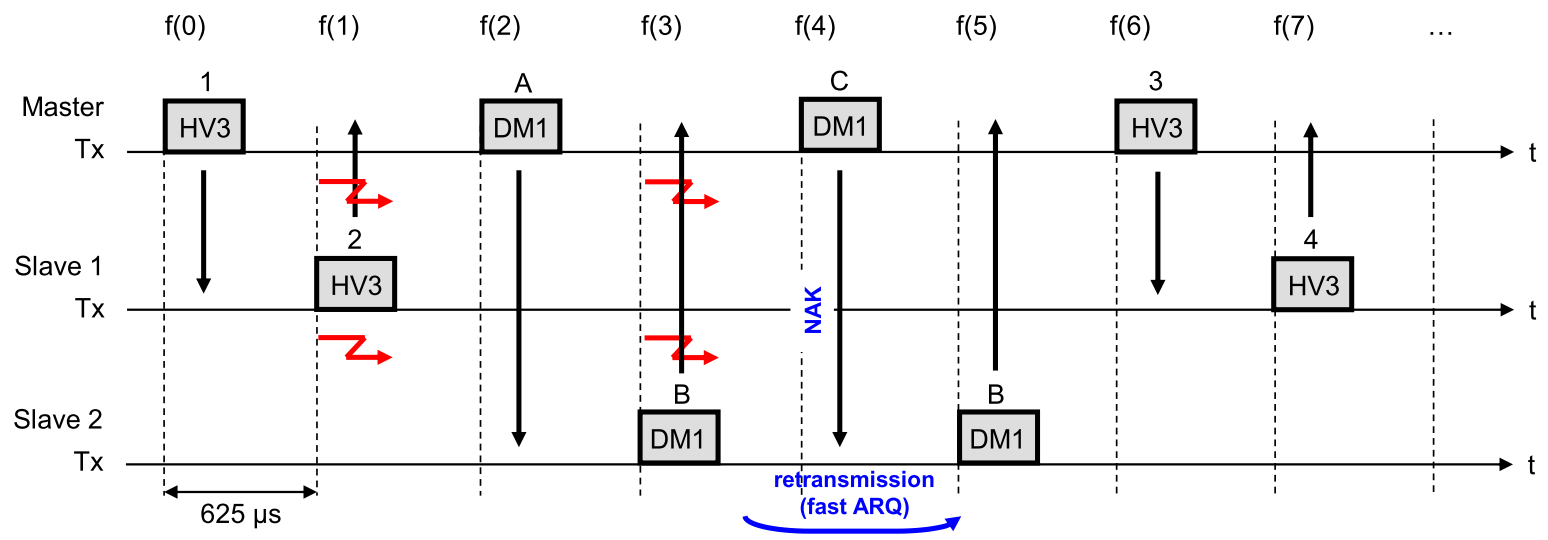
\includegraphics[width=16cm]{./bilder/bt-packet-transmission.png} 
	\end{minipage} \\
 

	HVx packets are periodically transmitted (e.g. in every 7th slot) to guaranty a time bounded 64 kb/s voice 
	service. HVx packets are not retransmitted (in contrast to the eSCO packets EVx 
	packets). 

	The slave has to retransmit the DM1-packet B because it receives a NAK in the header 
	of DM1-packet C. This procedure is also called fast Automatic Repeat reQuest ARQ. \\
	
	\textbf{Example:} Calculation of net data rate R for 3-DH1 (Up- or Downlink, with total 6 slots) \\
	$R = \frac{U_{pl}\cdot 8 \text{bit}}{N_{slots}\cdot T_{slot}} = \frac{83\cdot 8 \text{bit}}{6\cdot 625\mu s} = 177$kbps \\
	Where: $U_{pl}=$ User Payload [bytes], $N_{slots}=$ Total number of slots, $T_{slot}=625\mu$s = Slot time
	
	
	
\section{Bluetooth LE/Smart}
	\begin{tabular}{ll}
		\parbox{10cm}{
			\begin{itemize}
				\item Brand new protocol stack compared to BR/EDR
				\item Target: Ultra low power application which runs with coin cell battery
				\item Works with 40 channels of 2 MHz in the 2.4 GHz band
				\item GFSK Modulation (Gaussian Frequency Shift Keying)
				\item Bitrate of 1 Mb/s on the air interface (0.2 Mb/s application data rate)
				\item client server architecture
				\item Only star networks possible
				\item Uses advertising events on 3 channels to broadcast data without established connection (no hopping, using 3 channels in sequence)
				\item Data exchange with frequency hopping on 37 data channels when connection established
				\item Inquiry time: 20ms - 10s (due to advertisement interval)
				\item Connecting time: $\leq 3$ms after advertisement
				\item Radio range 10-20m indoor, somewhat larger than BT-BR/EDR (power class 2) due to more sensitive receiver
				\item Peak current consumption $\leq 15$mA to run on coin cell battery
				\item Power consumption 1-50\% of Bluetooth BR/EDR, depending on use case
				\item BLE is not voice capable
			\end{itemize}

		}	
		& \parbox{8cm}{
			\fbox{ 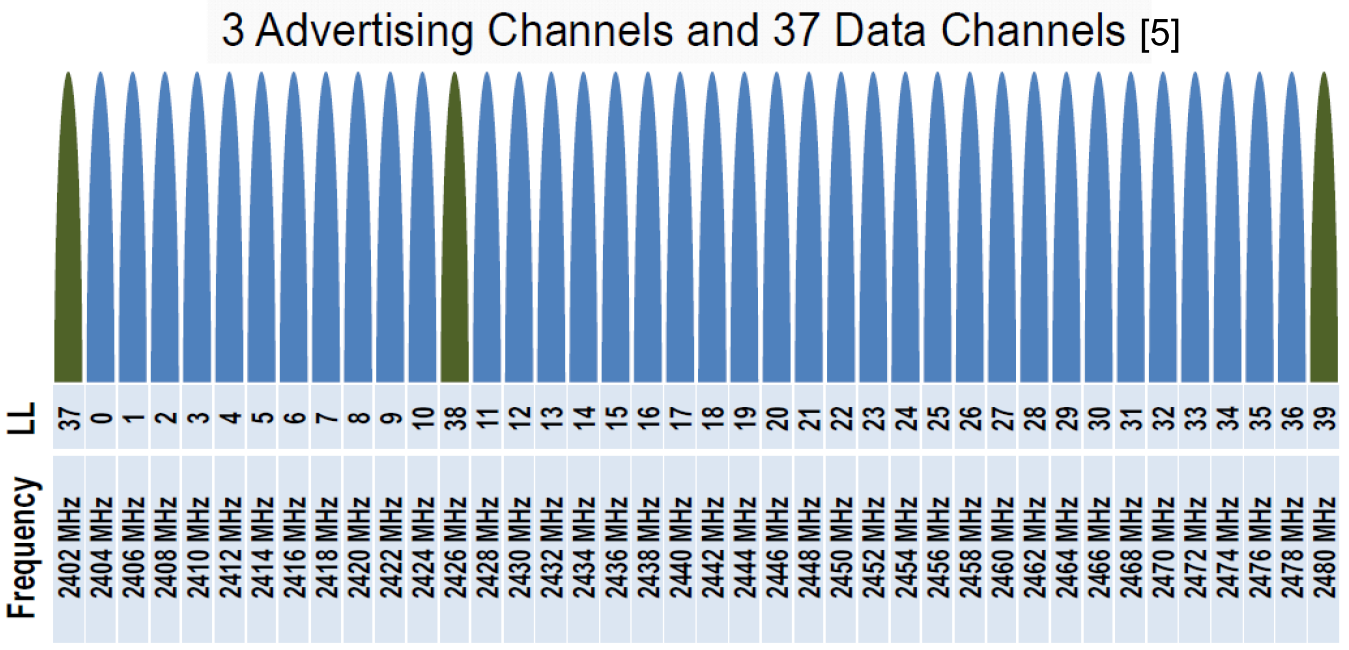
\includegraphics[width=8cm]{./bilder/ble-channels.png}} \\ BLE advertising and data channels }
	\end{tabular}
	
	\subsection{Topology}
		\begin{tabular}{ll}
			\parbox{9cm}{
				\fbox{ 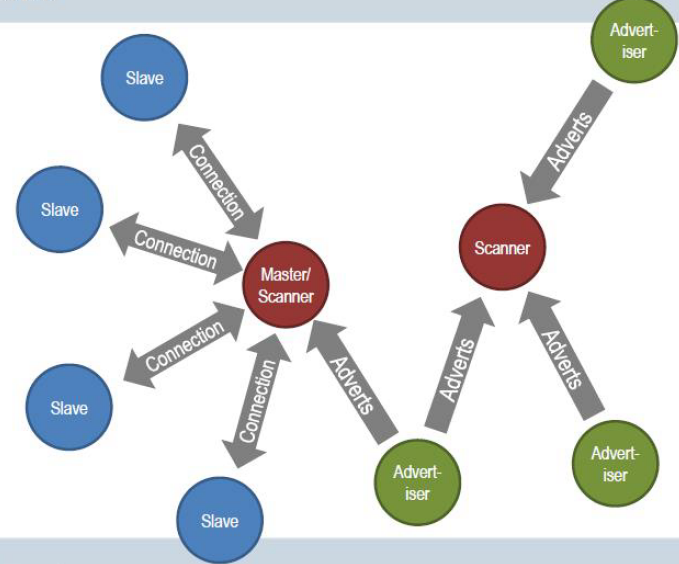
\includegraphics[width=8cm]{./bilder/ble-topology.png}} \\ BLE Topology 
			}	
			& \parbox{9cm}{
				Maximum 4 slaves are available at the moment on the market. However, the BLE standard doesn't define a maximum number of slaves.
				
				Compared to BT-BR/EDR the master is communicating on different frequencies with the slaves.
				With BLE it is not possible to have scatternet anymore.
			}	
		\end{tabular}
		
	\subsection{Message Sequence Chart}
		\begin{tabular}{ll}
			\parbox{11cm}{
				This is an example for a Message Sequence Chart between a Bluetooth LE advertiser and a Bluetooth LE initiator, assuming that 
				\begin{itemize}
					\item the advertising interval is 1s (and the random advertising delay can be neglected)  
					\item the host of the initiator requests a connection at $t = 1.5$s with a connection interval of 1s  
					\item the (adaptive) data channel hop sequence is 15, 32, 24, 17, 10, 5, 6, 11, 19, ...  
					\item the first connection event starts 1s after the last advertising event started  
					\item the slave latency is 3 (the slave answers to the first connection packet)  
					\item master and slave send data packets with empty PDU if required and no data is available   
					\item the host of the slave requests to send a notification with a newvalue at $t = 7.5$s 
				\end{itemize}
			}
			& \parbox{7cm}{
				\fbox{ 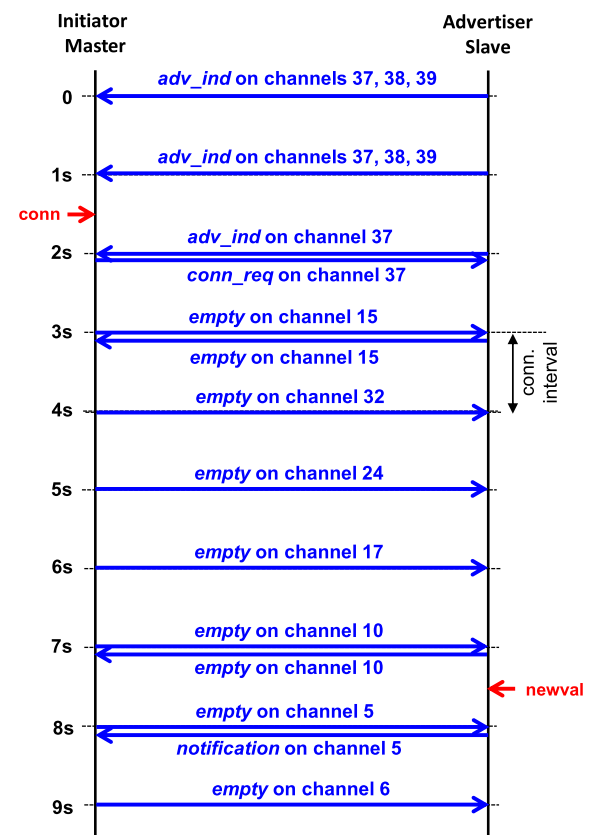
\includegraphics[width=7cm]{./bilder/ble-msc.png}}
			}	
		\end{tabular}
			
	\subsection{Scanning}
		\begin{tabular}{ll}
			\parbox{9cm}{
				The \textbf{scanner} is listening for advertising channel packets from devices that are advertising. A passive 
				scanner is only listening, while an active scanner may request an advertiser to send additional information. \\
				
				\textbf{Advertising Channel PDU types} \\
				\begin{tabular}{|l|c|c|} \hline 
					\textbf{Advertising event type} & \textbf{SCAN} & \textbf{CONNECT} \\ \hline \hline
					& \multicolumn{2}{|c|}{allowed}  \\ \hline
					ADV-IND & YES & YES \\ \hline 
					ADV-DIRECT-IND & NO & YES \\ \hline 
					ADV-NONCONN-IND & NO & NO \\ \hline 
					ADV-SCAN-IND & YES & NO \\ \hline 	
				\end{tabular} }
			& \parbox{9cm}{
				\fbox{ 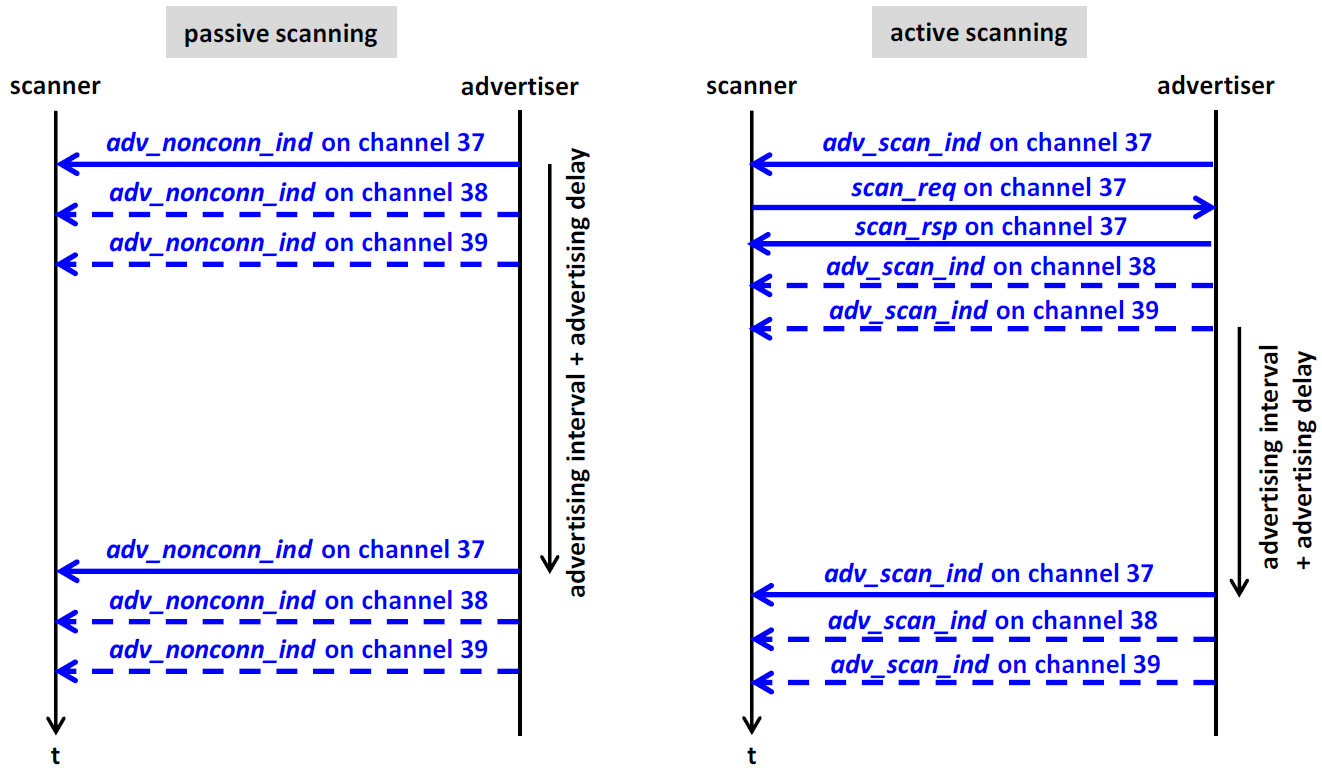
\includegraphics[width=9cm]{./bilder/ble-scanning.png}}
			}
		\end{tabular}	
			
\section{Wireless Networks}
\begin{tabular}{|l|l|l|}
	\hline
	\textbf{Typ} & \textbf{Beschreibung} & \textbf{Standarts}\\
	\hline
	PAN & Personal Area Network & Bluetooth, ZigBee, Ultrawideband\\
	\hline
	WLAN & Wireless Local Area Network & WLAN, Wi-Fi\\
	\hline
	MAN & Metropolitan Area Network & WiMAX\\
	\hline
	WWAN & Wireless Wide Area Network & GPRS, EDGE, UMTS, LTE\\
	\hline
\end{tabular}
\subsection{PAN - Personal Area Networks \formelbuch{264}}
\begin{tabular}{|l|l|l|l|l|l|l|} \hline
name of system & RF & b/w per channel & data rate  & tx power	& distance  & modulation  \\
\hline \hline
Bluetooth 802.15.1 & 2.4\,GHz	& 1\,MHz	& 1\,Mbit/s	      & 100\,mW	 & 80\,m	& GFSK \\ \hline
ZigBee 802.15.4	   & 868\,MHz,& 2\,MHz	& 20\,kbit/s,     & 100\,mW  & 75\,m	& BPSK, \\
              	   & 915\,MHz,& 2\,MHz	& 40\,kbit/s,     & 100\,mW  & 75\,m	& BPSK,  \\
                   & 2.4\,GHz & 2\,MHz	& 250\,kbit/s     & 100\,mW  & 75\,m	& O-QPSK \\ \hline
DECT	             & 1.9\,GHz	& 1.728\,MHz & 1152\,kbit/s	& 100\,mW	 & 300\,m	& GFSK \\ \hline
\end{tabular}\\

\textbf{Bluetooth \formelbuch{264}}\\
\textbf{ZigBee \formelbuch{264}}\\
\textbf{Ultrawideband (UWB)\formelbuch{265}}

\subsection{WLAN - Wireless Local Area Networks}
Wi-Fi is defined as any wireless local area network (WLAN) products that are based on the Institute of Electrical and Electronics Engineers' (IEEE) 802.11 standards. \\

\begin{tabular}{|l|l|p{3cm}|p{3cm}|l|l|} \hline
Technology & Spectrum & Max. Bandwidth & Modulation & MIMO streams & Max Data Rate
\\ \hline \hline
802.11  & 2.4\,GHz  & 22 MHz           & FHSS, DSSS  & n.a. & 1-2\,Mbps  \\ \hline
802.11a    &   5\,GHz  & 20 MHz           & OFDM      & n.a. & 54\,Mbps \\ \hline
802.11b    & 2.4\,GHz  & 22 MHz          & DSSS     & n.a. & 11\,Mbps \\ \hline
802.11g    & 2.4\,GHz  & 20 MHz           & OFDM, DSSS   & n.a.  & 54\,Mbps \\ \hline
802.11n   & 2.4 \& 5\,GHz & 20 or 40 MHz	     & OFDM  & 4 & 65-300\,Mbps \\ \hline
802.11ac   &   5\,GHz  & 20 - 160 MHz 	  & OFDM	& 8 & 86-780\,Mbps \\ \hline
\end{tabular}

\subsubsection{MAC Layer}
WiFi uses Carrier Sense Multiple Access (CSMA) on the MAC Layer. The station ready to send data starts sensing the medium and 
if the medium is free for the duration of a DIFS, the station can start sending directly. If the medium is busy, the station has to 
wait for a free DIFS and additionally wait a random back-off time (collision avoidance, multiple of slot-time of 20us). In case 
another station occupies the medium during the backoff time waiting, the backoff counter stops at the current value and continue
decreasing from that value at the next round (fairness). 

With the first transmission attempt the random slot for the backoff-procedure is chosen between 0 - $CW_{min}$, where $CW_{min}$ for 11b and g is 31, for 11n it's 15. \\
On any further attempt the random slot is chosen between 0 - 63, then 0 - 127, ... 0 - $CW_{max}$. \\
$CW_{max}=1023$ slots (20 ms), afterwards the frame is discarded on the MAC Layer. \\

\begin{tabular}{ll}
	\parbox{7cm}{
		\textbf{Example:} \\
		\begin{itemize}	
			\item  no RTS- and CTS-packet are used
			\item  DIFS = 50 us, SIFS = 10 us and a slot time = 20 us
			\item  the transmission period for each data packet is 500 us
			\item  the transmission period for each ACK-packet is 140 us
			\item  STA1 has a data packet pending and a remaining backoff of 20 slots
			\item  STA2 has a data packet pending and a remaining backoff of 5 slots
			\item  STA3 gets a request to send a packet from a higher layer at t = 750 us
			and chooses a random backoff of 10 slots
		\end{itemize}
	}
	& \parbox{11cm}{
		\fbox{ 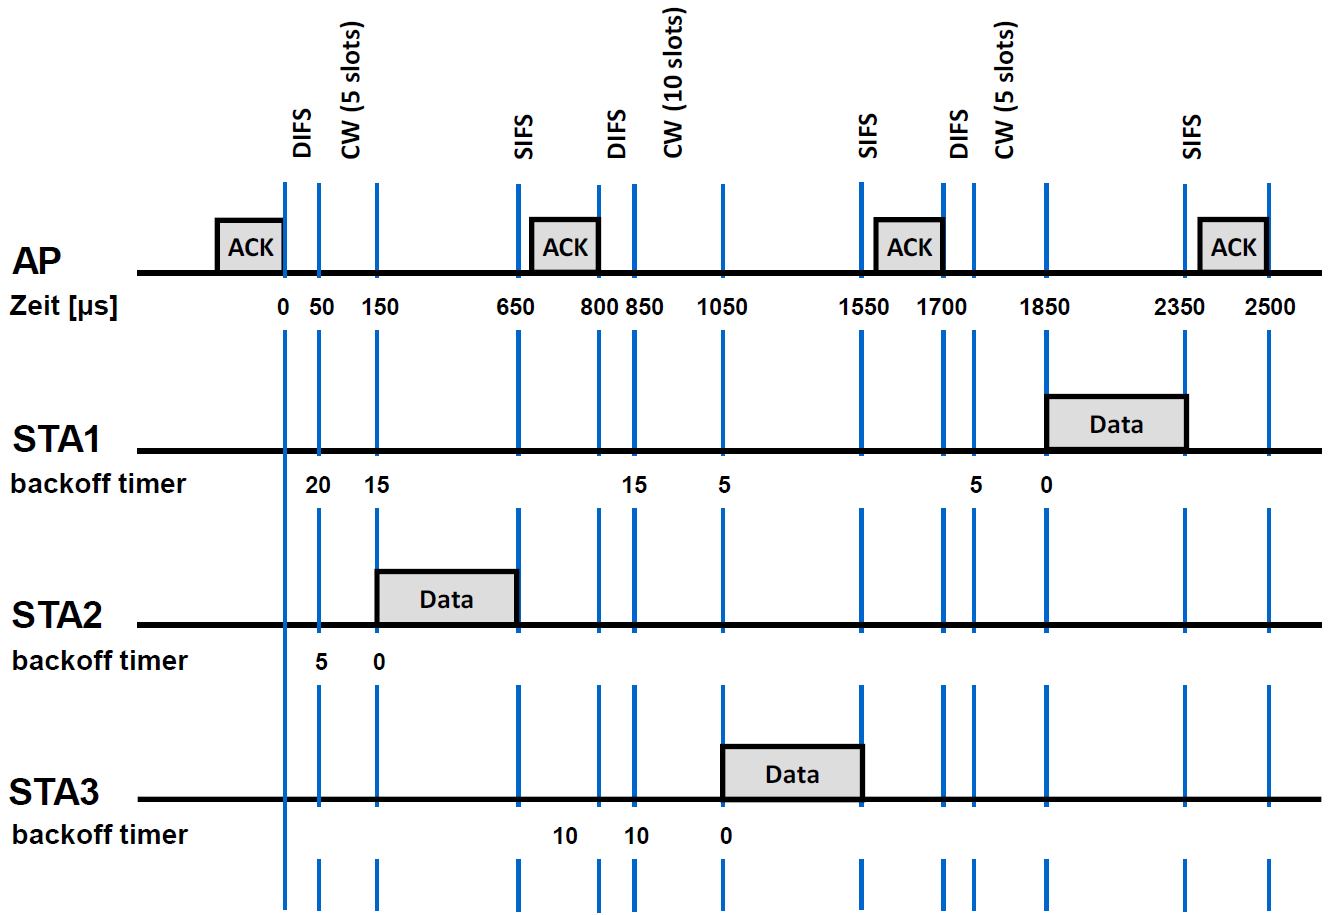
\includegraphics[width=11cm]{./bilder/wlan-csma.png}} \\ 
	}
\end{tabular}	
	
\subsubsection{PHY Layer of IEEE 802.11g}
	\begin{tabular}{ll}
		\parbox{11cm}{
			For the PHY Layer of 802.11g standard OFDM with 52 subchannels is used (4 pilot channels and 48 data channels). 
			The symbol rate is 250 kSps and therefore the symbol period is $T_{symbol}=4\mu$s. The 11g standard defines several modulation
			and coding schemes with different data rates. Which one of these can be used depends on the actual SNR
			(the higher the SNR, the higher the modulation). 				
		}
		& \parbox{7cm}{
			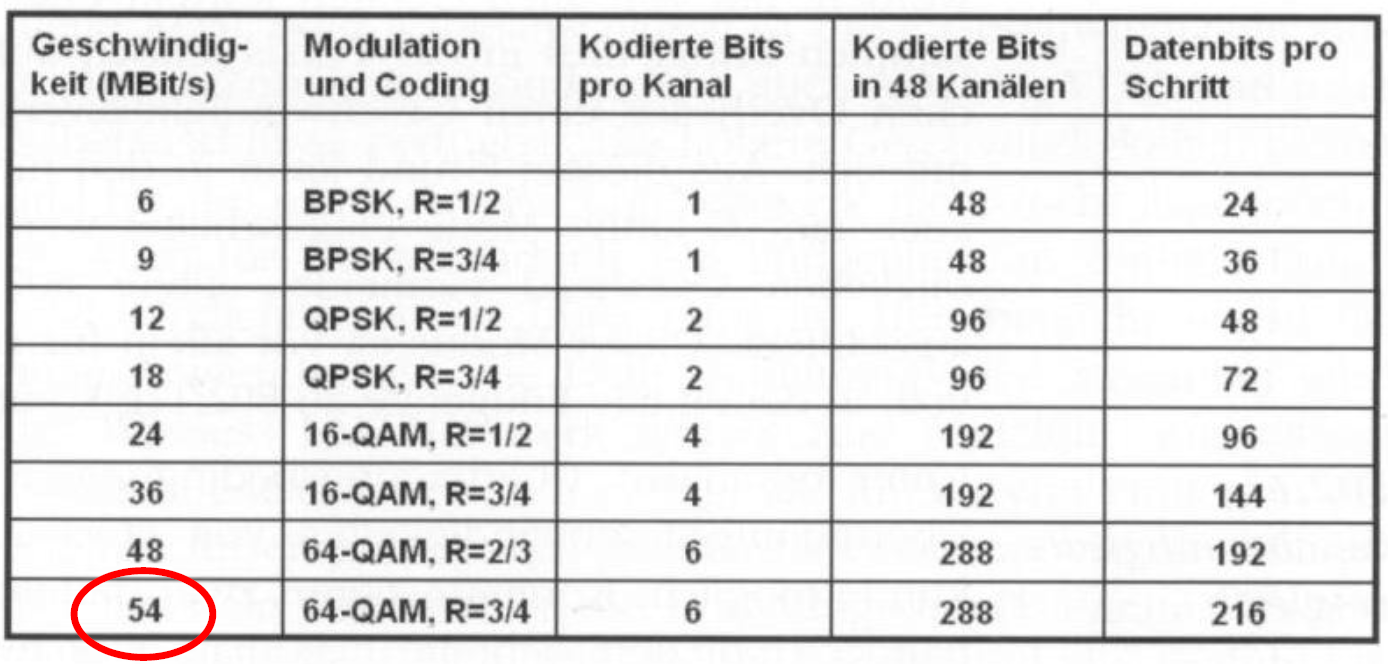
\includegraphics[width=7cm]{./bilder/wlan-phy.png} \\ 
		}
	\end{tabular}
	
	The data rate R is calculated as follows: $R=\frac{N_{OFDM}\cdot BPC}{T_{symbol}}\cdot R_{FEC}$ \\
	Where $N_{OFDM}=$Number of OFDM data channels $=48$ , $BPC=$Bits per channel , $R_{FEC}=$Coding rate \\
	
	Some 802.11g or 11a devices might have two Antennas. However, this is not intended for MIMO but rather
	for Antenna Diversity, i.e. improve the received signal by reducing the probability of deep fading. 

	In some cases there is the possibility to activate the option "G only". By doing so, the backwards
	compatibility with 11b devices is deactivated, but due to less interworking overhead the performance
	increases of about 40\%.
	
%\subsection{MAN - Metropolitan Area Networks}

\section{GPS - Global Positioning System \formelbuch{181}}
\subsection{Einführung\formelbuch{181}}  
        Ziele von NAVSTAR-GPS=NAVigation System with Timing and Raning Global
        Positoining System:
        
    \begin{minipage}{12.3cm}	  
        \begin{liste}
            \item 3-D Ortung bei stehenden oder bewegenden Objekten überall auf der
            Erde oder in Erdnähe (meist bis 18km über Meer)
            \item Geschwindigkeitsberechnung
            \item unlimitierte Teilnehmerzahl (alle gleichzeitig)
            \item Zeitinformation
            \item unabhängig von Wetter und Klima
            \item grosse Sicherheit gegenüber internen und externen (mutwilligen)
            Störungen
            \item grosse genauigkeit (Position RMS Ziel/heute bei 30/2.5m ; Speed RMS
            0.3/0.1$\frac{m}{s}$; time RMS 10/30ns)    
        \end{liste}
		Bezüglich des RF-Signals:
		\begin{liste}
	    	\item grosse Bandbreite (Frequenzen über 1GHz)
	    	\item kleine Antennen (hohe Frequenzen)
	    	\item kleiner Übertragungsverlust (tiefe Frequenzen)    
	    \end{liste}
		$\Rightarrow$Kompromis beim L-Band (1-2 GHz)		
    \end{minipage}
    \begin{minipage}{6cm}
        \begin{tabular}{|l|l|}
            \hline
                \textbf{Eigenschaft} & \textbf{Wert} \\
            \hline
	            Trägerfrequenz
	                & 1.57542 GHz \\
	            $d_{\text{Sat-Earth}}$
	                & 20'192 km \\
	            $r_{\text{Earth}}$
	               & $6.37103\cdot 10^{6}$\,m \\
	            $t_{\text{Sat-Umlauf}}$
	               & 11\,h 57\,m 57.26\,s $\approx$ 12\,h \\	         
	            C/A Clock
	               & 1.023\,MHz \\
	            Data Clock
	               & 50\,Hz \\
	               
            \hline
        \end{tabular}
    \end{minipage}    

\subsection{Konzept\formelbuch{183}}
	Das Konzept basiert auf der Fortplanzungsgeschwindigkeit der Wellen. So wird
	ein Signal mit der aktuellen Zeit geschickt. Mit dem Zeitunterschied
	zwischen User Gerät und dem Empfangenen Signal kann man die Distanz zu den
	Satelliten (SV) berechen. So kann man aus 3 Distanzen die eigene Position
	berechen. Da jedoch die Userzeit nicht zwingend mit der des SVs
	überreinstimmt,  braucht man einen zusätztlichen SV.
\subsection{Systemübersicht\formelbuch{183}} 

    \begin{minipage}{13cm}
    \subsubsection{Satelliten Konstellation}    
	    Für eine gleichmässige Abdeckung kreisen die Satteliten in 6 unterschiedlichen
	    Orbits um die Erde. Diese haben alle eine Höhe von 20`192km, das
	    heisst, dass die Satelliten 12h pro Umdrehung oder 1d um den gleichen Punkt auf
	    der Erde erreichen zu haben (Da sich die Erde auch dreht). Die Orbits sind
	    $55^\circ$ vom Equator geneigt und haben je $60^\circ$ Abstand voreinander.    
    \end{minipage}
    \begin{minipage}{6cm}    
        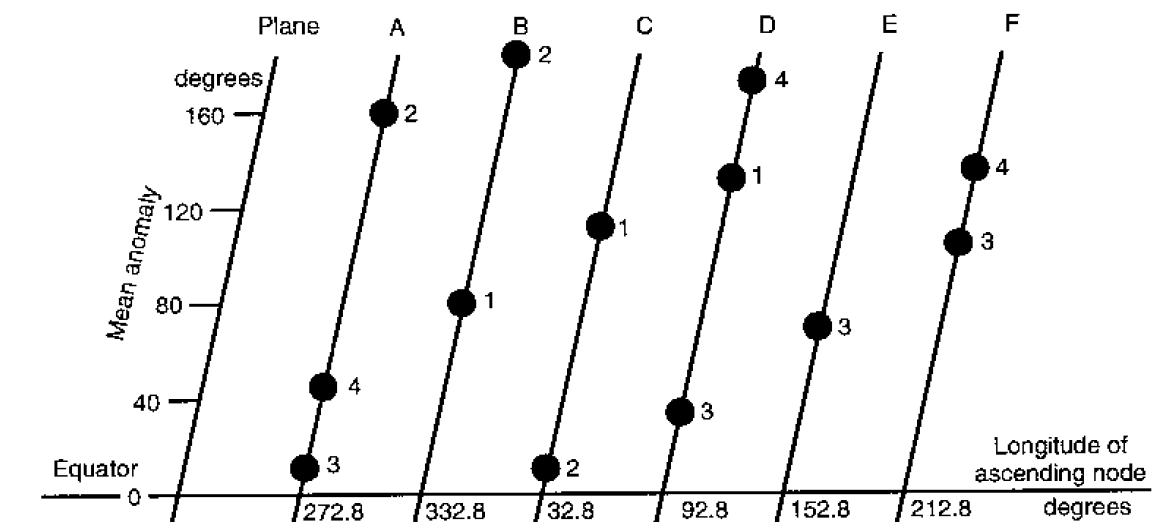
\includegraphics[width=6cm]{./bilder/GPS-SatConstellation.png}    
    \end{minipage}
	
	\subsubsection{control network}
	Die drei Hauptaufgaben des von der USA gestellten Kontrollnetzwerk sind:
	\begin{liste}
    	\item Überwachung der SV-Bewegungen
    	\item Überprüfen des SV- clocks
    	\item Die Zeitsynchrinisation der SV
    \end{liste} 
\subsection{Signal Charakteristik\formelbuch{187}}
	\subsubsection{Übersicht}
		\begin{minipage}{9cm}
      		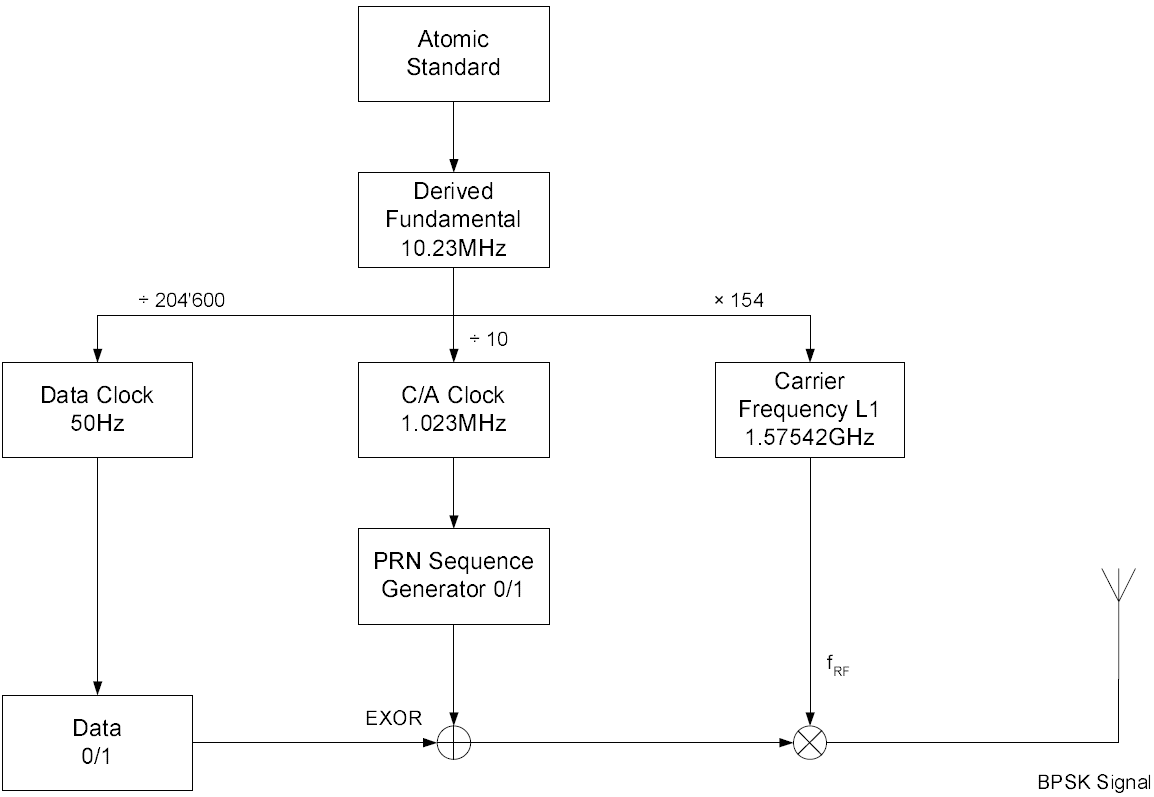
\includegraphics[width=9cm]{./bilder/GPS-Signalaufbau}
        \end{minipage}
		\begin{minipage}{10cm}
        	Alle SV senden auf der gleichen Frequenz. Dadurch muss das
        	Signal CDMA- codiert sein.\\
        	Datensignal: Die Datenrate ist nur 50 bits/s. Für alle Informationen	
        	braucht man 12.5min. Es werden folgende Informationen übertragen:
        	\begin{liste}
            	\item SV- Zeit
            	\item Ephemeriden: genaue Positionsdaten des SV
            	\item almanac: ungefähre Positionsdaten aller SVs
            	\item Zeit Korrektur
            	\item Ionosphäre Daten
            	\item Gesundheitsinformation des SVs
            \end{liste}
		\end{minipage} 
	\subsubsection{PRN Sequenz: Gold code}
		\begin{minipage}{10cm}
        	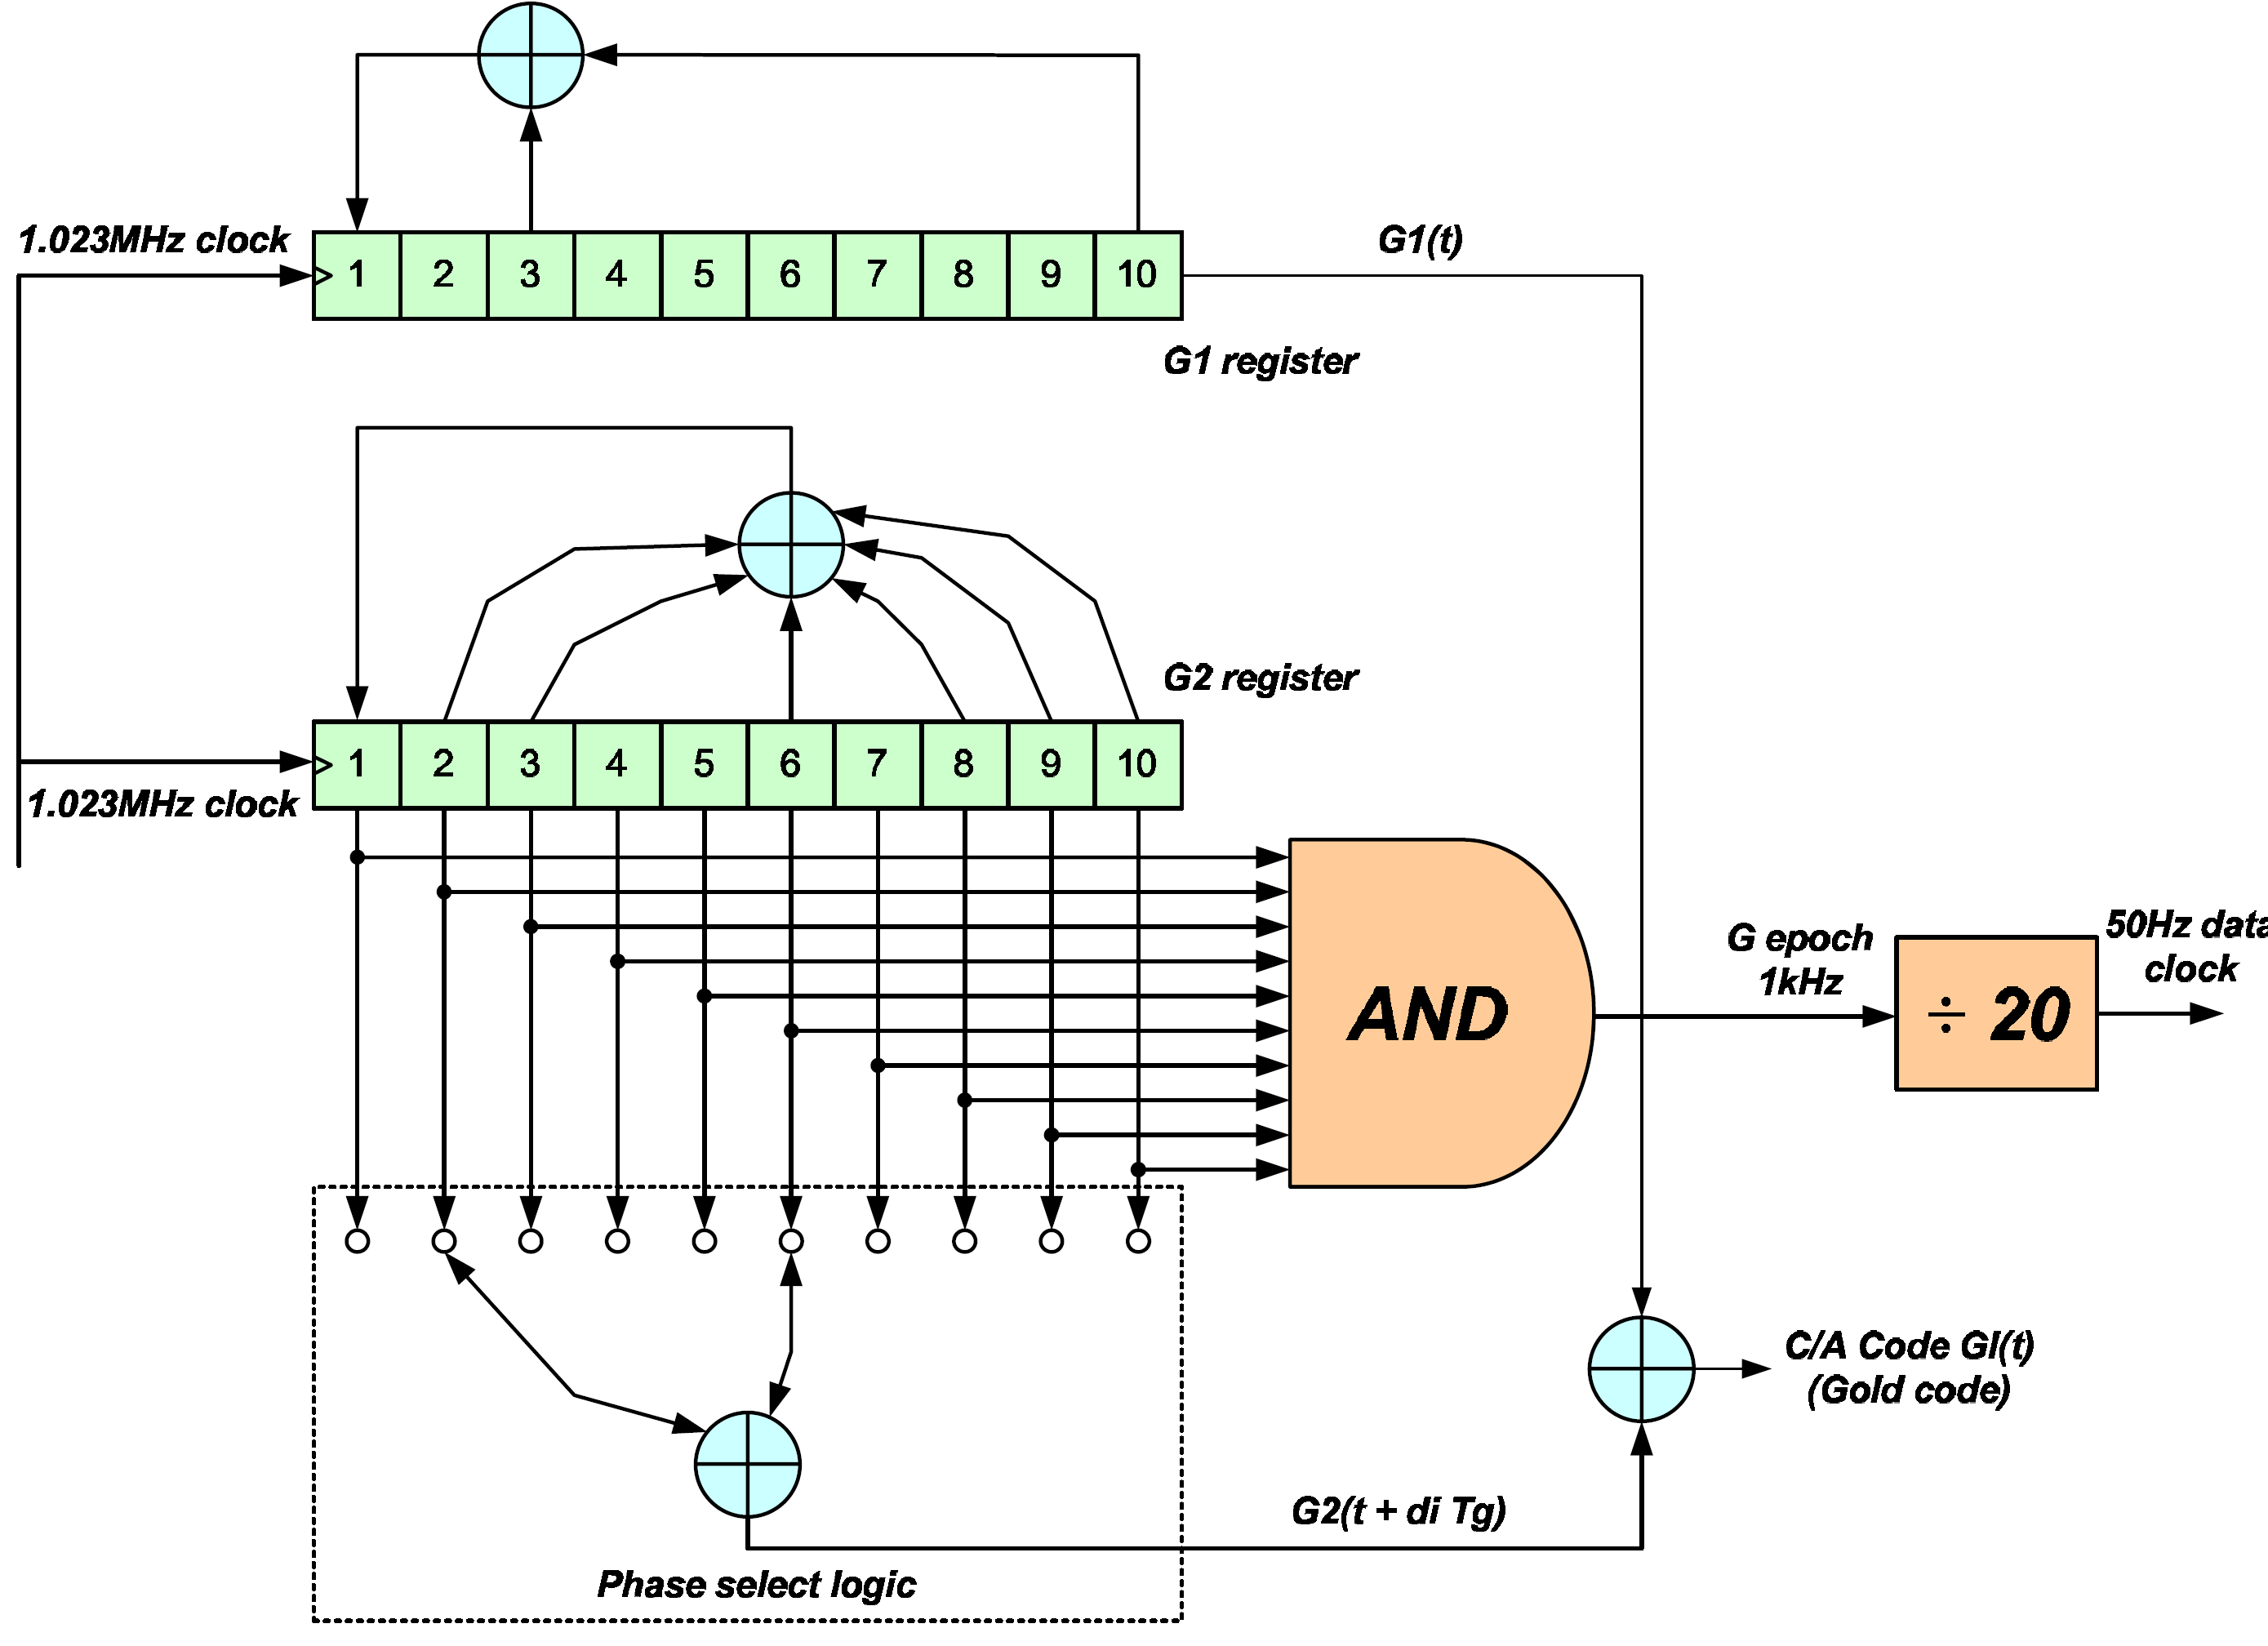
\includegraphics[width=9cm]{./bilder/GPS-Gold.png}
        \end{minipage}
		\begin{minipage}{8cm}
        	Jeder SV hat genau eine Sequenz
        	von $2^n-1=2^{10}-1=1023$ Bits. Dadurch wird die PRN Sequenz alle
        	1ms wiederholt. Pro Datenbit hat es genau 20 Sequenzen, dass heisst es
        	wird jeweils nur ganze Sequenzen mit $\pm$1 multipliziert werden\\
        	Eine Gold- Sequenz wird durch zwei 10 Bit Register erzeugt, welche
        	unterschiedlich mit EXOR rückgekoppelt werden. Beim schlussendlichen
        	Signal wird der Ausgang des ersten Register mit dem verzögerten
        	Ausgang oder durch EXOR verknüpte Bit des zweiten Register verknüpft.
        	Je nach Verzögerung bzw. EXOR- Verknüpfung kann man auf den Satellit
        	schliessen.
        \end{minipage}
			
	\subsubsection{Signalleistung}
		Der free-space loss ist:\\
		$$L [dB] = 147.6 +20\log_{10}(Frequenz)+20\log_{10}(Distanz) = -147.6 +
		20\log_{10}(1.57542\cdot10^9) + 20\log_{10}(2.5785\cdot10^7) = 184.6 dB$$\\
		Die Empfangsleistung ist:\\
		$$P_{\text{rx}} = P_\text{sende} + \text{antenna gain} - \text{free space
		loss} - \text{atmosphere loss} = 43.4 + 13.4 - 184.6 - 2 \approx
		-130\,\text{dBm}$$\\
		Die Rauschleistung ist bei einer Bandbreite von ca 2.046MHz:\\
		$$P_\text{Noise}=-174dB+10\log_{10}(2.046\cdot10^6\text{Hz})\approx110\text{dBm}$$\\
		Das ergibt ein SNR von ca. -20dB. Durch Korrelation kann jedoch die SNR
		theoretisch um einen Faktor von $10\log_{10}(2.046\cdot10^6)=63.1\text{dB}$
		verbessert werden.
	\subsubsection{Korrelation}
		\begin{minipage}{6cm}
        	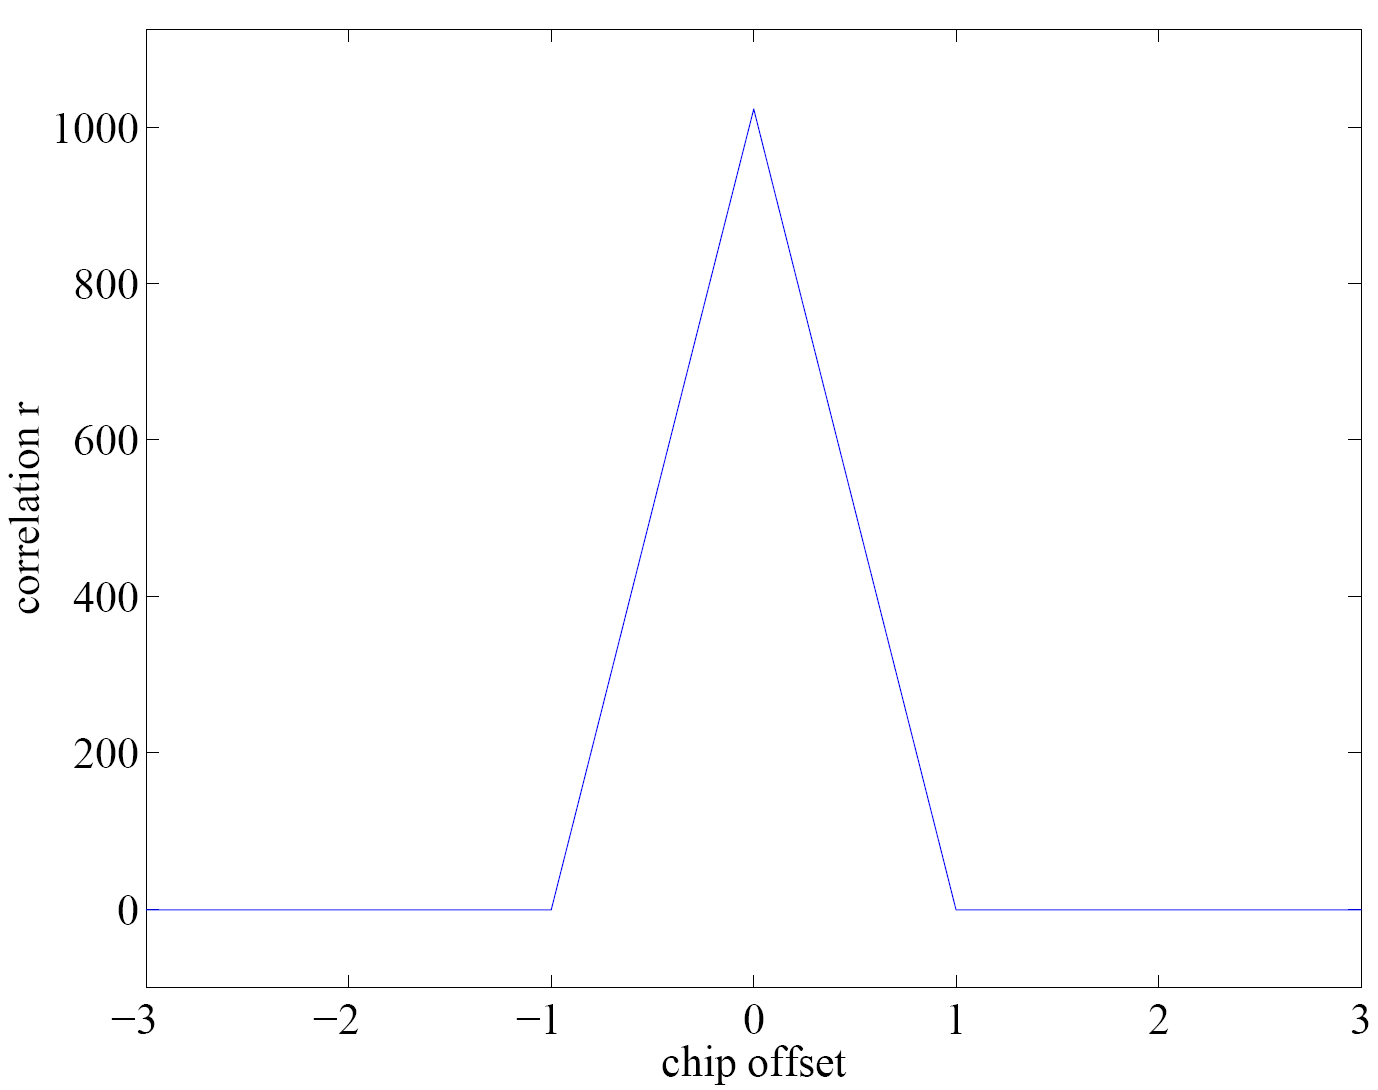
\includegraphics[width=6cm]{./bilder/GPS-Autokorrelation.png}
        \end{minipage}
		\begin{minipage}{6cm}
        	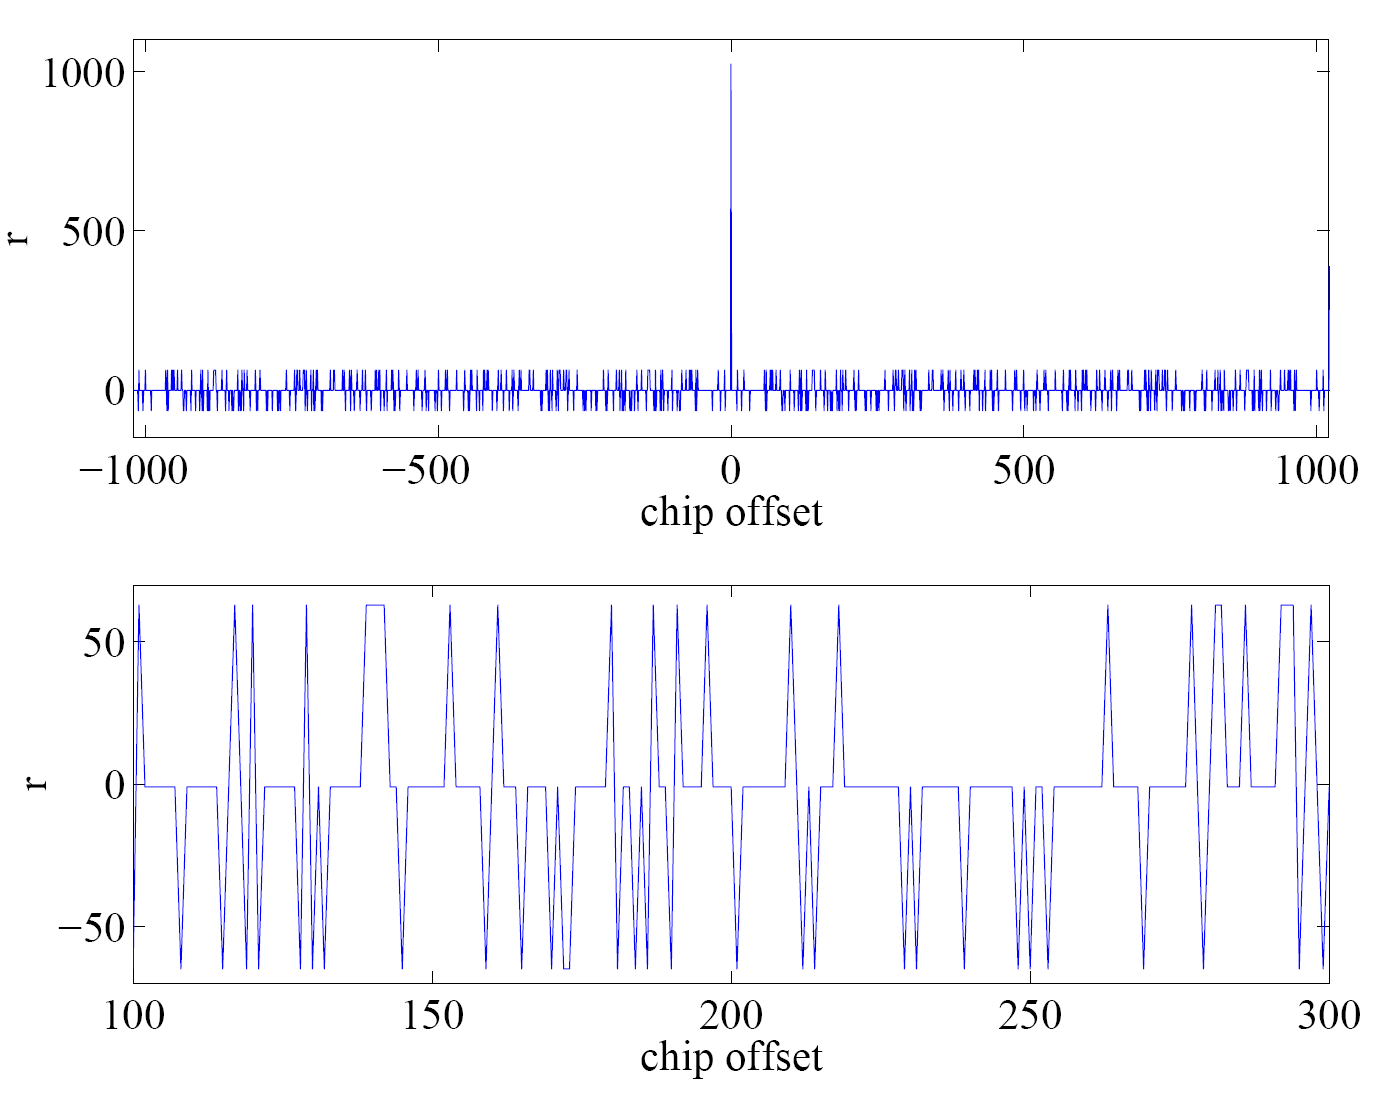
\includegraphics[width=6cm]{./bilder/GPS-Autokorr_Sequenz.png}
        \end{minipage}
		\begin{minipage}{6cm}
        	Der Peak der Autokorrelation ist 1023 hoch. Da eine Sequenz immer eine
        	ungerade Anzahl an Bits hat, ist sonst der Wert bei der
        	Auto- wie auch bei der Kreuzkorrelation -1. Ausserdem können
        	auch die Werte +63 und -65 vorkommen.\\
        	Falls ein Satellitensignal um
        	$20\log_{10}(\frac{1023}{63})=23.9\text{dB}$ stärker ist, kann eine
        	Verwechslung auftreten.
        \end{minipage}

\newpage

\subsection{Empfänger Architektur\formelbuch{194}}
	\begin{minipage}{10cm}
		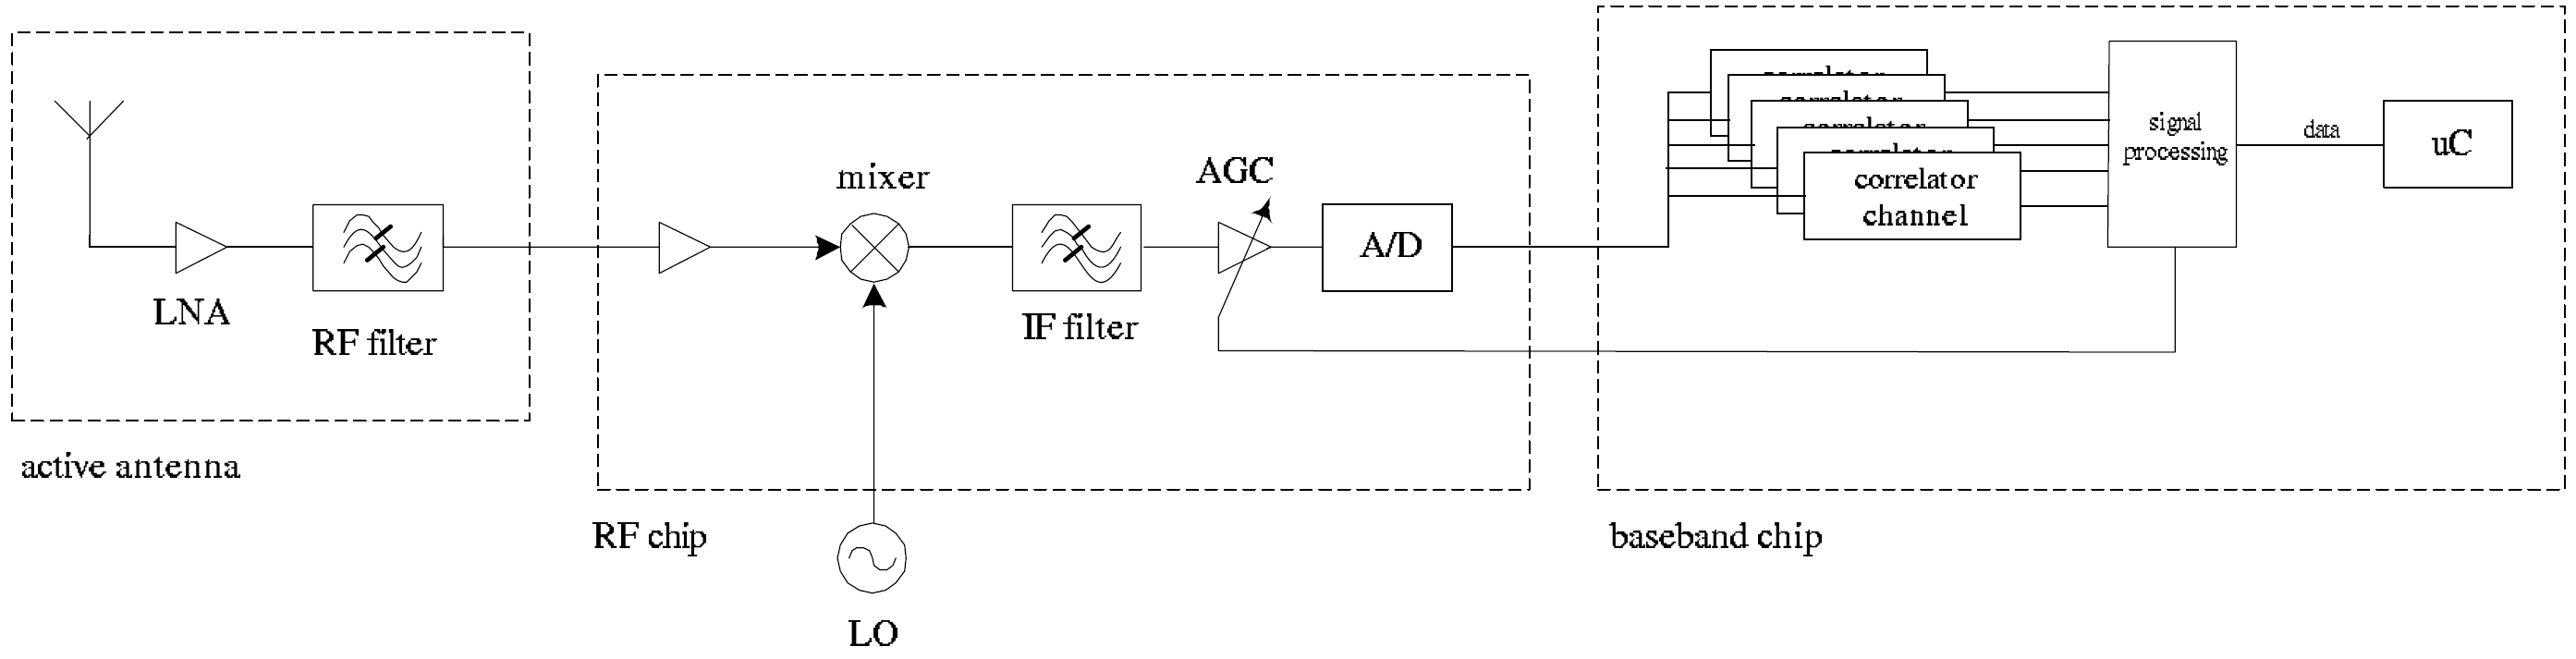
\includegraphics[width=10cm]{./bilder/GPS-Empfangsarchitecture.png}
	\end{minipage}
	\begin{minipage}{8cm}
    	\textbf{Antenna}: Die Antenne muss zirkular polarisiert (Gegenuhrzeiger)
    	sein(RHCP). Um nur das normale Band empfangen zu können (1.57542GHZ),
    	braucht sie nur eine kleine Bandbreite. \\
    	\textbf{LNA}: Meist wird dieser direkt im Antennen Gehäuse integriert.
    \end{minipage}\\
	\textbf{AGC}: Im Gegensatz zu anderen wireless Anwendungen wird hier der
    	AGC nur verwendet, um die Unterschiedlichen LNA auszugleichen (zB. wenn
    	keine bzw. eine aktive Antenne gebraucht wird)\\
    \begin{minipage}{8cm}
    	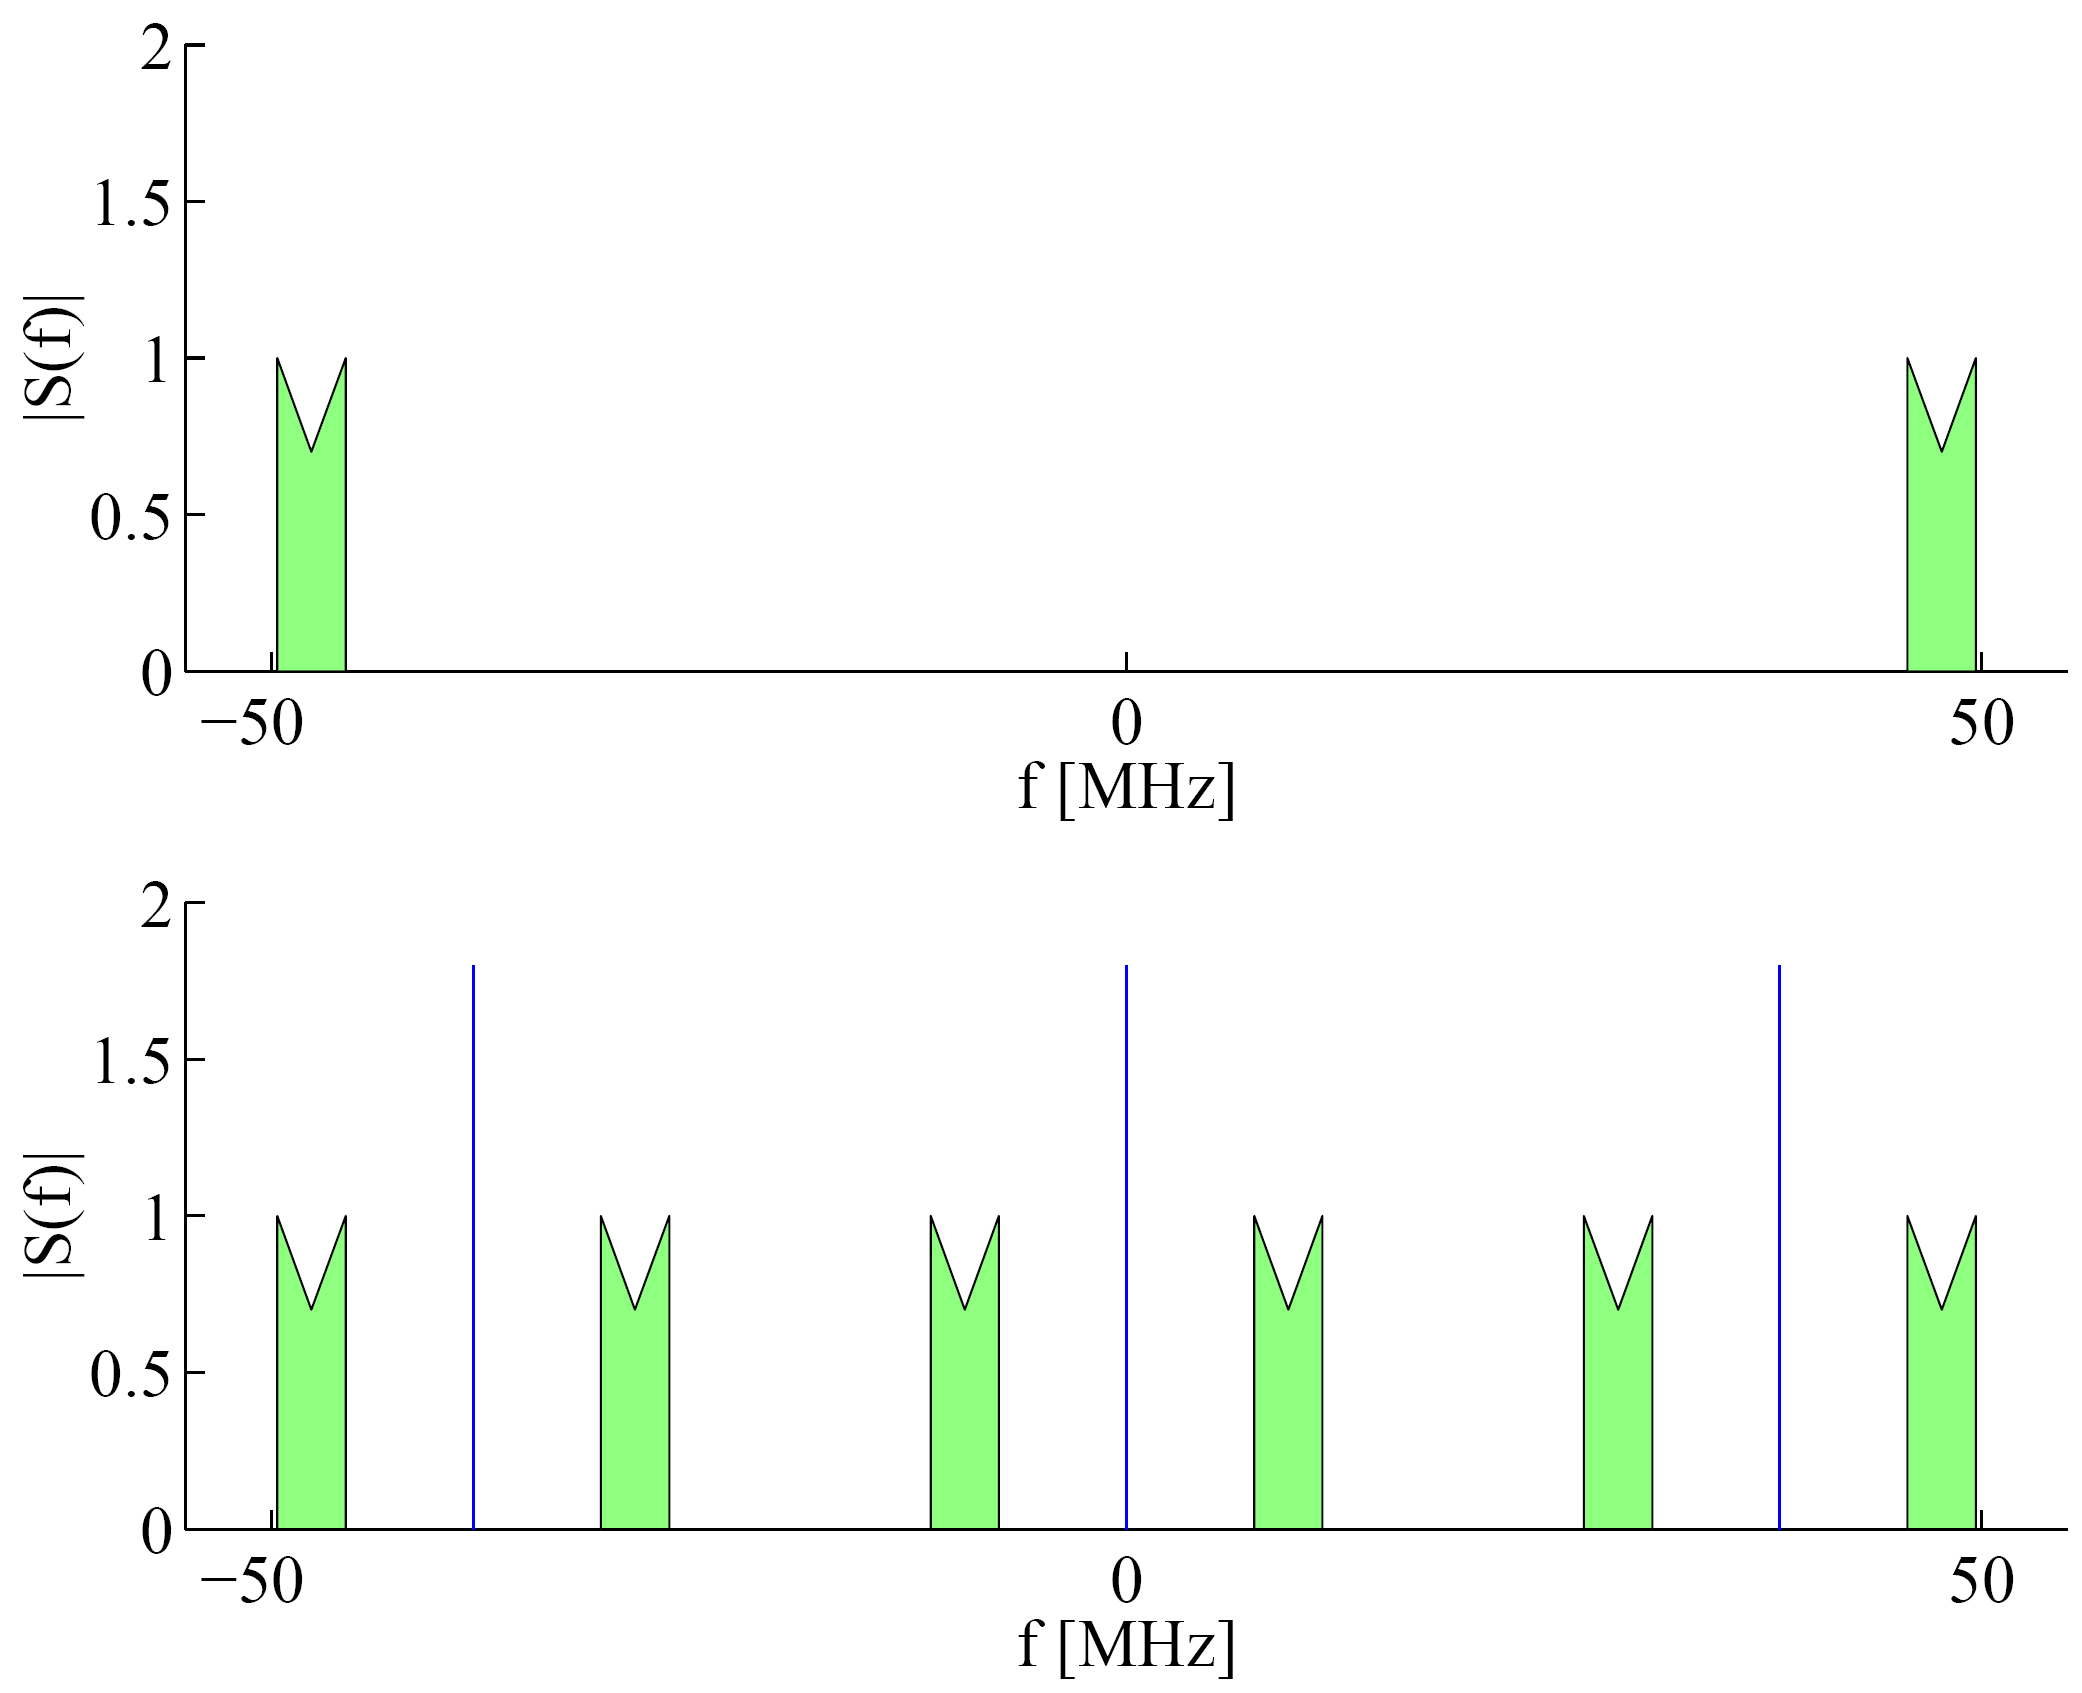
\includegraphics[width=6cm]{./bilder/GPS-Downsampling.png}
    \end{minipage}
	\begin{minipage}{9cm}
	    \textbf{ADC}: Wenn man das bekannte Nyquist-Gesetz erweitert zu $2B\leq
	    f_s$ kann man ein bandbegrenztes Signal mit dem Abtasten auch noch
	    runtermischen. Dafür muss noch folgende Bedingung zur Abtastfrequenz
	    eingehalten werden:\\
	    $$\frac{2f_u}{n}\leq f_s\leq\frac{2f_l}{n-1}\text{ mit }|
	    f_l=IF-\frac{B}{2};f_u=IF-\frac{B}{2}$$
	   	
    \end{minipage}\\
	IF von 47.65MHz; $f_s=38.194$MHz ergibt $IF_{Digital}=47.65-38.194=9.456$MHz
    
\subsection{GPS und die Relativitätstheorie\formelbuch{202}}
	\begin{minipage}{10cm}
    	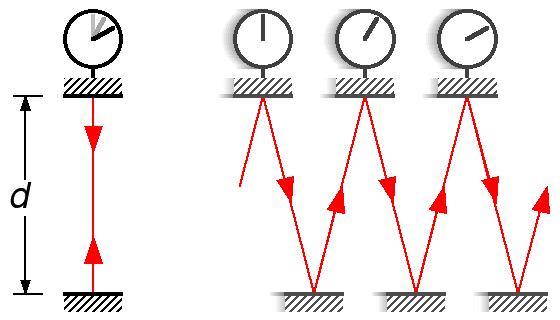
\includegraphics[height=4.5cm]{./bilder/GPS-Relativitaettheory.png}\\
    	Lichtuhrversucht für die Spezielle Relativitätstheorie
    \end{minipage}
	\begin{minipage}{8cm}
		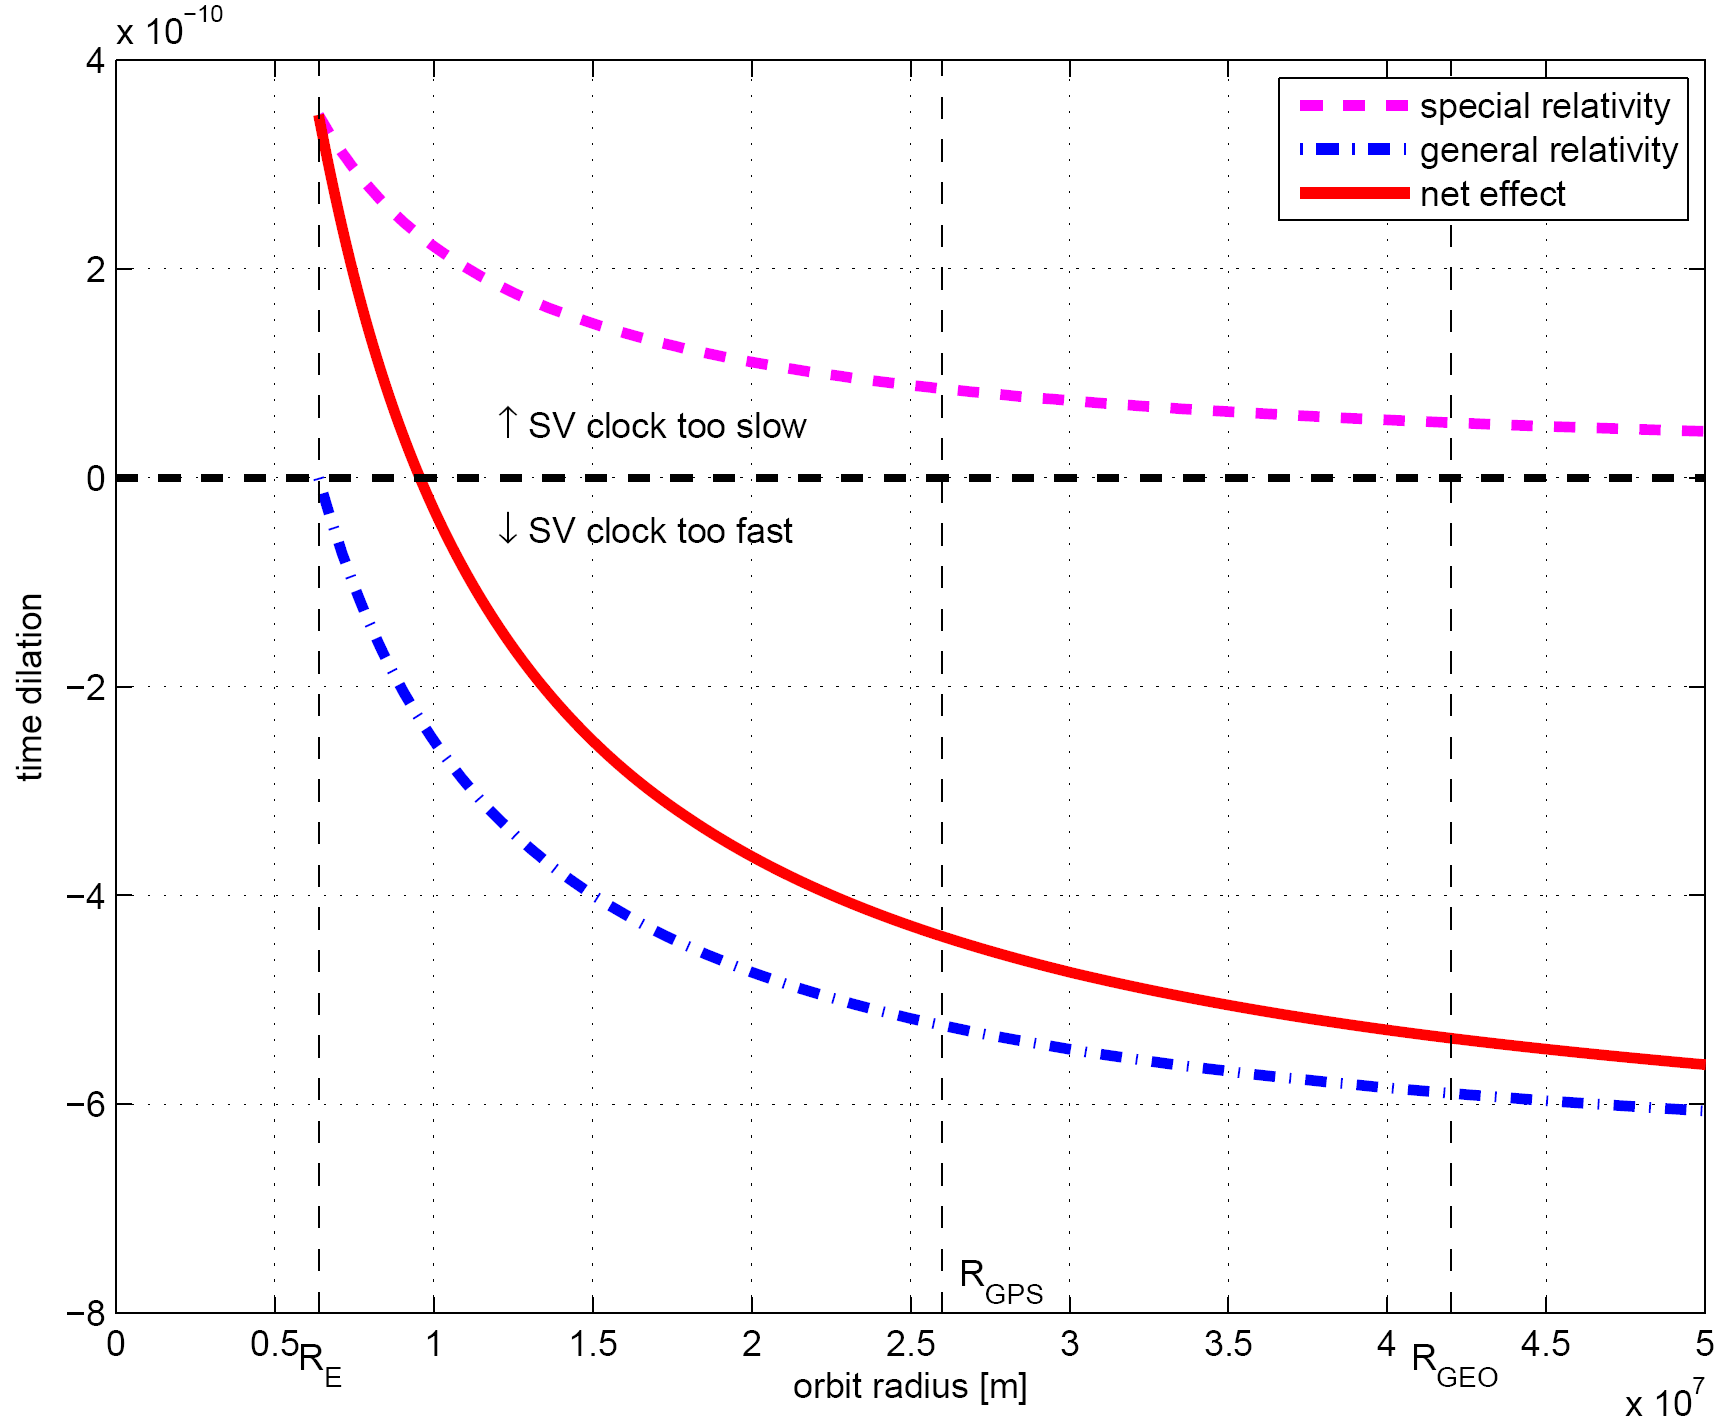
\includegraphics[height=5cm]{./bilder/GPS-ZeitKorrektur.png}\\
		Übersicht der beiden wirkenden Zeitveränderungen
	\end{minipage}\\ \\
	Das Licht legt die Strecke d zurück löst einen Impuls aus und wird
	reflektiert, etc. (\textbf{spezielle Realtivitätstheorie}) \\
	$v=konst.\Rightarrow$ Zeit des bewegenden Objekts ist langsamer da eine
	grössere Strecke zurückgelegt werden muss 
	$ t'_{bew} = \frac{t_{ruh}}{\sqrt{1 - \frac{v^2}{c^2}}}$\\
	Für einen Satelliten ergibt sich dann:
	$t_{SV_1}= t_{Erde} \frac 1{\sqrt{1-\frac{g}{c^2}\cdot \frac{R_E^2}R}}$\\
	Die \textbf{generelle Relativitätstheorie} besagt, dass sich ein Clock
	langsamer ist, wenn er in einem Gravitationsfeld ist.\\
	$t_2 = t_0 \frac 1{\sqrt{1-\frac{2GM}{Rc^2}}} 
  	= t_0 \frac 1{\sqrt{1-\frac{g}{c^2}\cdot 2\frac{R_E^2}R}}$; 
  	$t_{SV_2}= t_E \frac{\sqrt{1-\frac{g}{c^2}\cdot 2 R_E }}
    {\sqrt{1-\frac{g}{c^2}\cdot 2\frac{R_E^2}R }}$\\
    Der totale Effekt ist, dass der Quarz des Satelliten mit nur
    10.229999995433MHz anstatt den 10.23MHz laufen muss.
    
\newpage    
\subsection{Acquisition\formelbuch{206}}

	\begin{center}
    	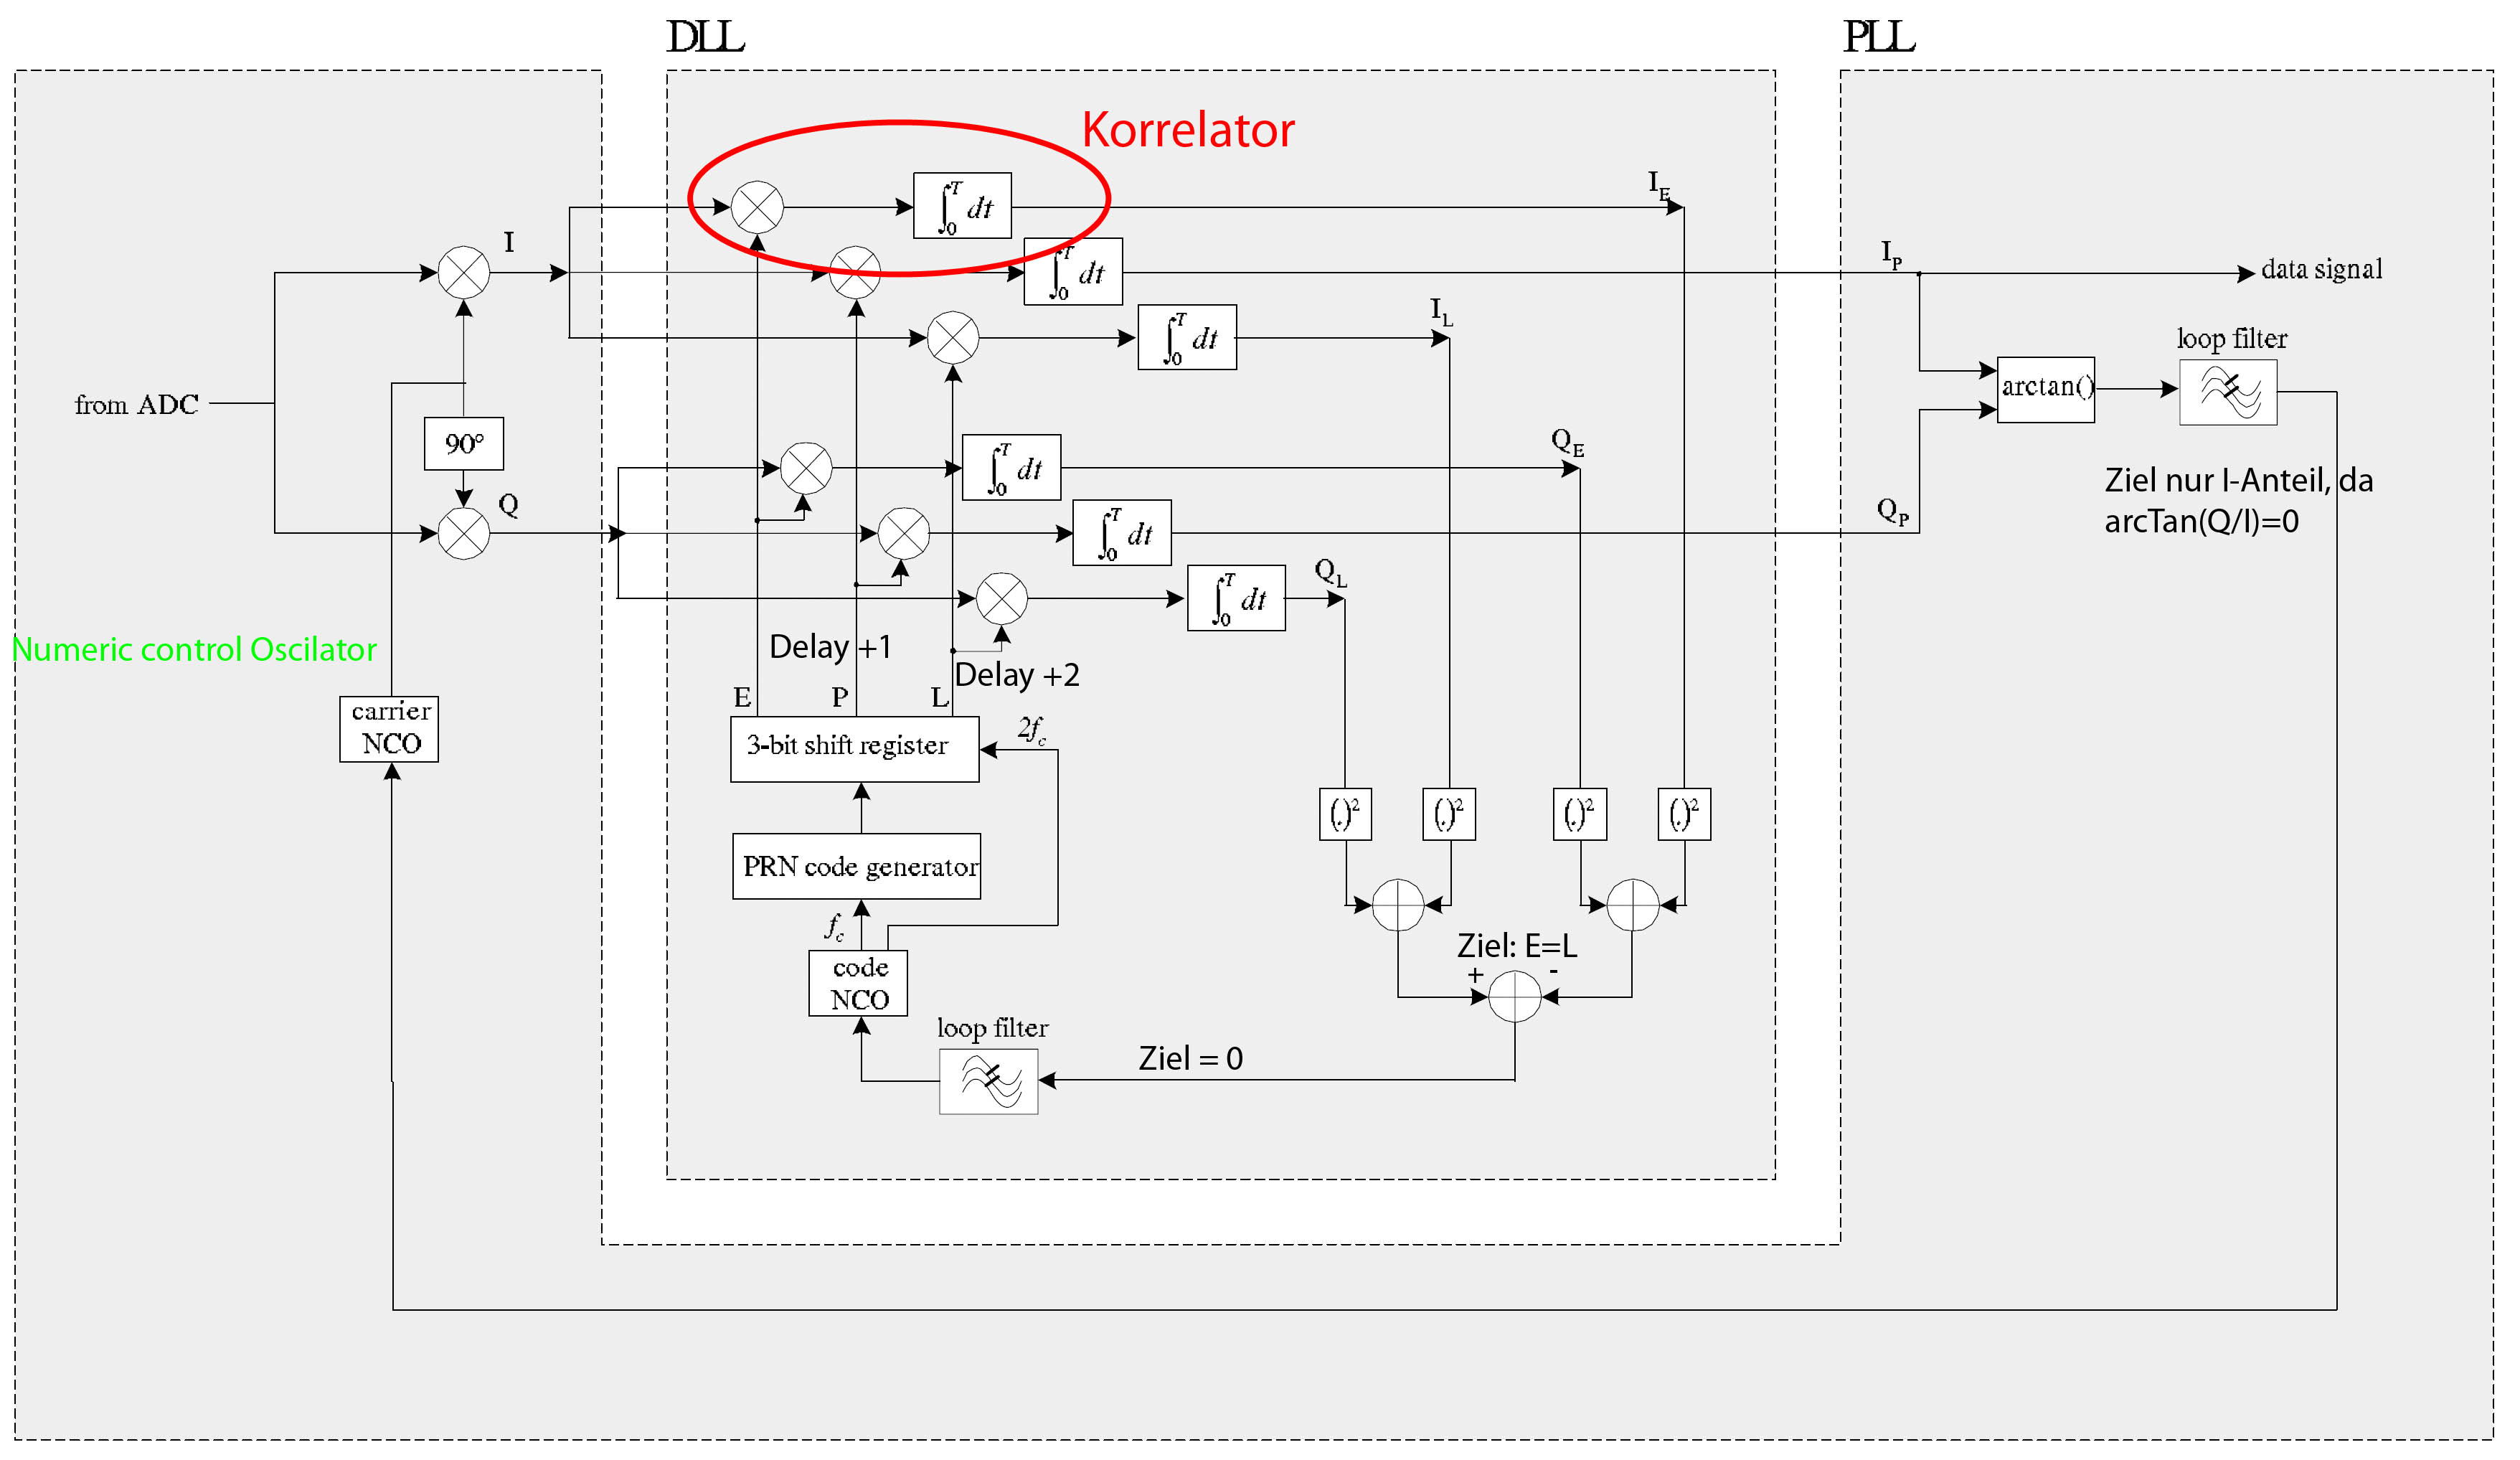
\includegraphics[width=14cm]{./bilder/GPS-Phasenlock.jpg}\\
    \end{center}

	Um die Satelliten zu finden muss in 3 Dimensionen gesucht werden:
	\begin{liste}
    	\item SV nummer: 	1 bis 28 (Anz: 28)
    	\item Code Phase: 	0 bis 2045 (halbe Bitbreite) (Anz: 2046)
    	\item Frequenz:		-35kHz bis +35kHz (Da ca 20ppm = 30kHz und $\pm$ 5kHz
    	Dopplershift in je 500Hz Schritten) (Anz:141)
    \end{liste}
	Das ergibt ohne jegliches Vorwissen für jeden Satellit $N=2046\cdot
	141=288486$ Möglichkeiten.\\
	Für die Auswertung muss $s=I_P^2+Q_P^2$ gerechnet werden (Korrelation) und eine
	Peakdedection vorgenommen werden.
\subsubsection{Chip resolution}
	\begin{minipage}{10cm}
	    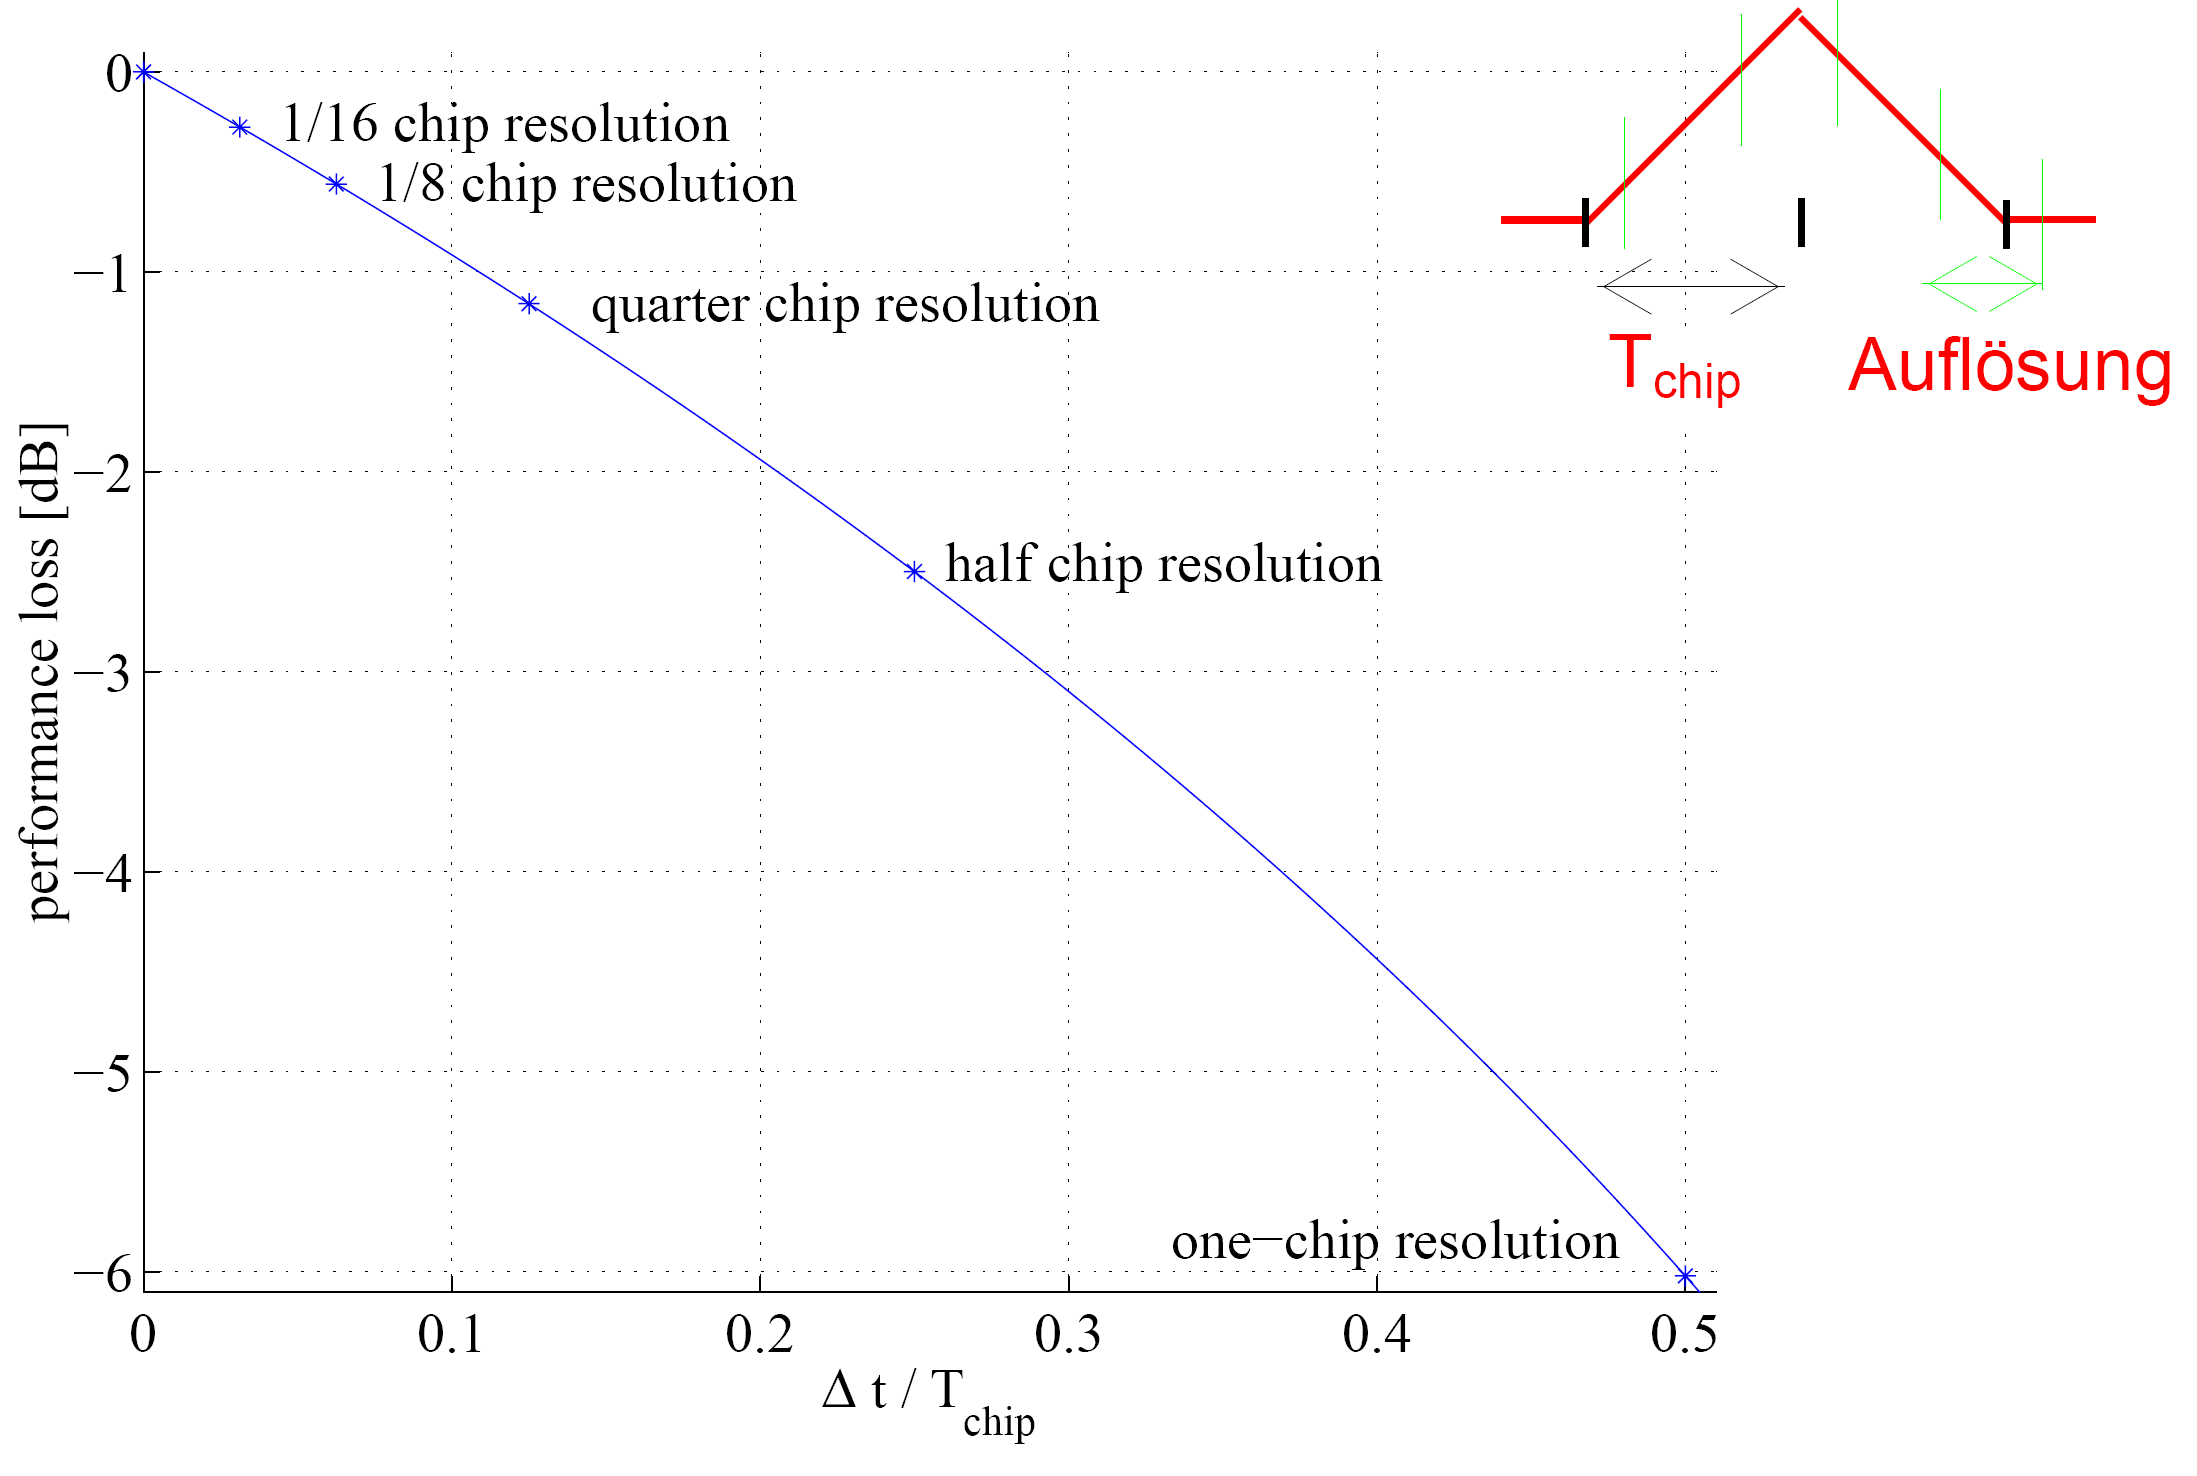
\includegraphics[width=8cm]{./bilder/GPS-ChipResolution.png}
    \end{minipage}
	\begin{minipage}{8cm}
    	Da die Phase nicht genau bekannt ist, treten bei der Dedektion des
		Spitztes der Autokorrelation Verluste auf, da nicht mehr das maximum erwischt
		wird.\\
		$\text{loss [dB]}= 20 \log_{10}\left(1-\frac{|\Delta
		t|}{T_{\mathrm{chip}}}\right)$\\
    \end{minipage}
\subsubsection{Frequenz resolution}
	\begin{minipage}{8cm}
    	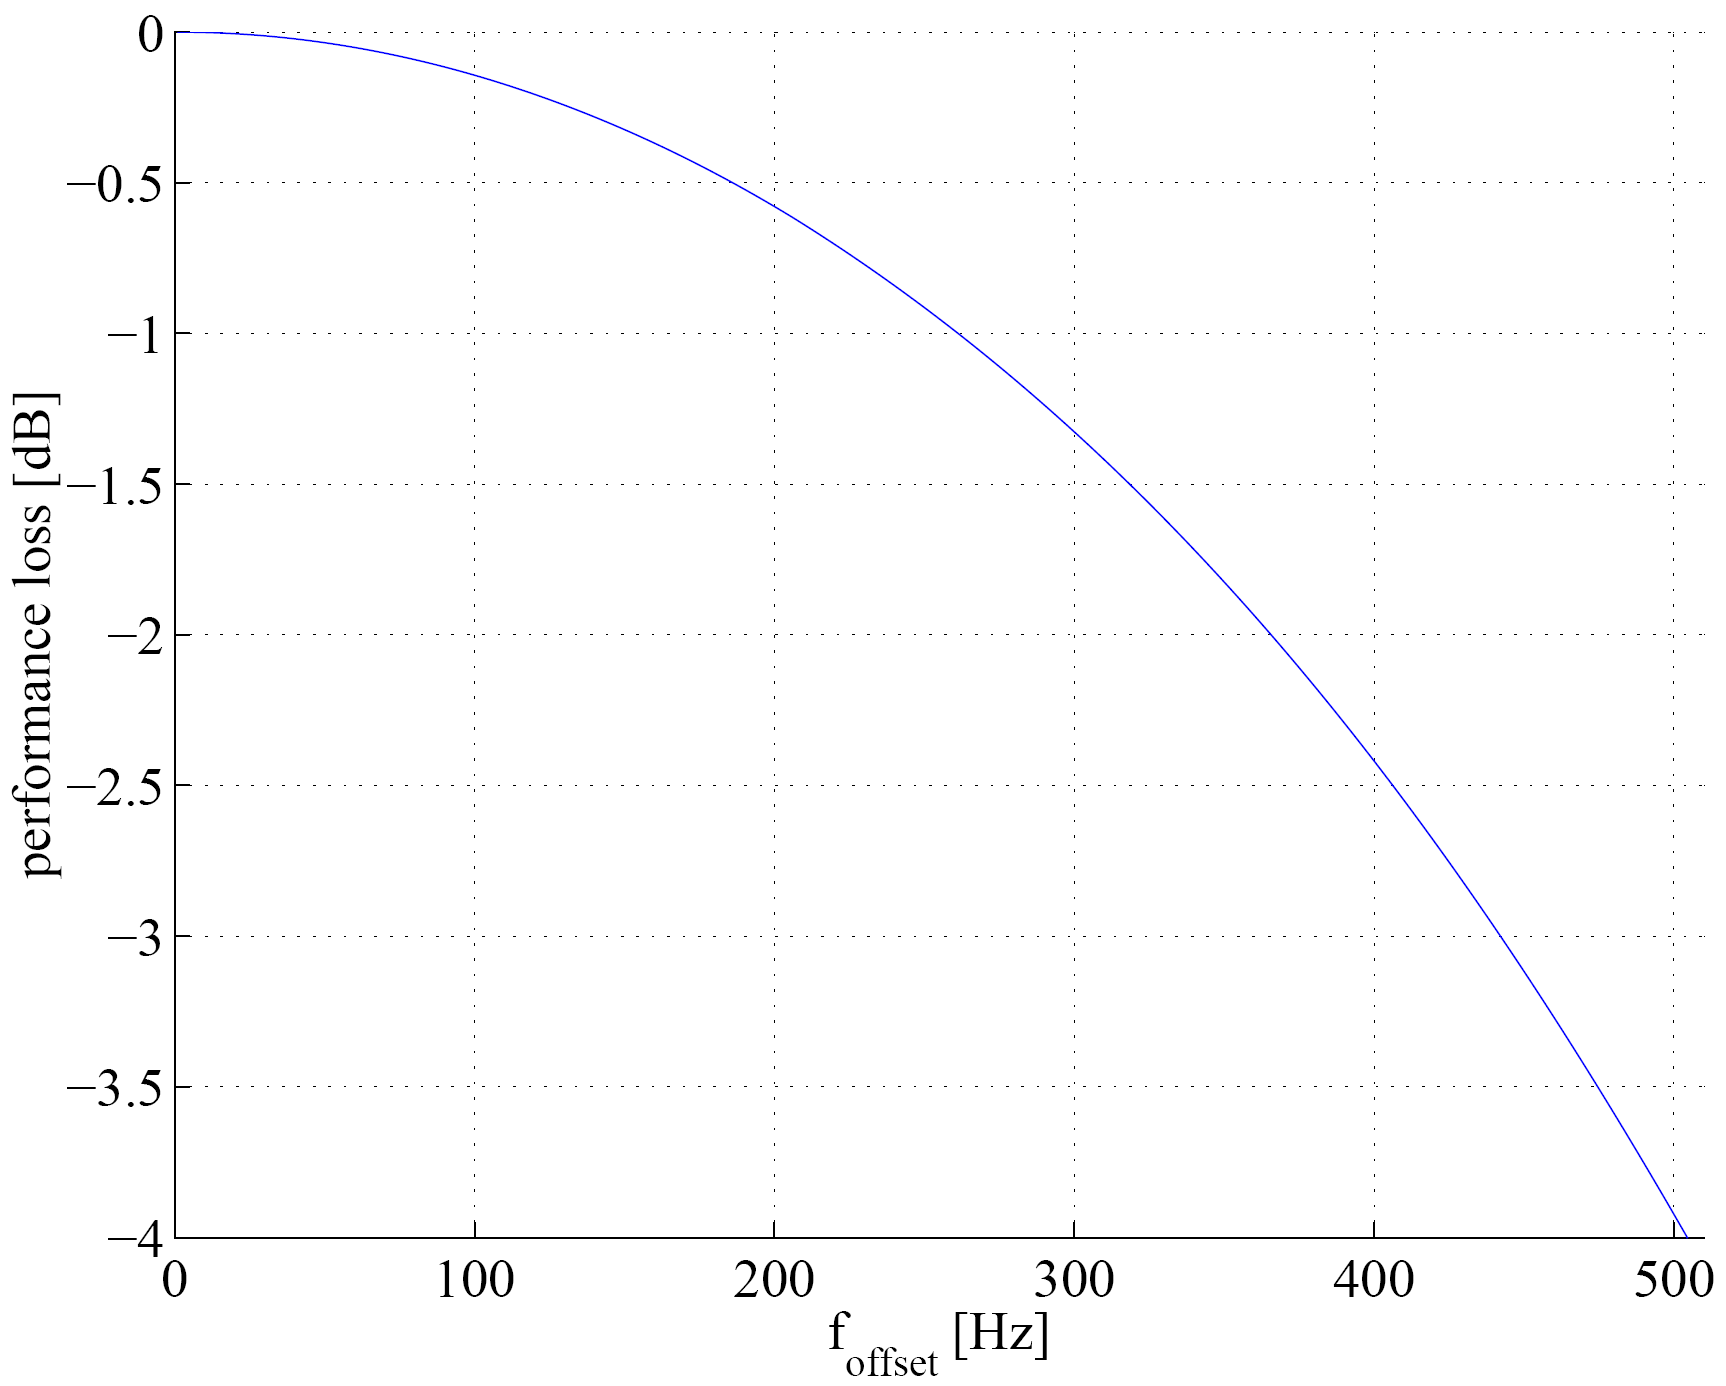
\includegraphics[width=6cm]{./bilder/GPS-FrequenzResolution.png}
    \end{minipage}
	\begin{minipage}{10cm}
	    Bei einem unbekannten Doppler Shift und einer unbekannten Frequenzabweichung
		treten in der Integration Verluste auf.\\
		$\text{loss [dB]}= 20 \log_{10} \frac{\sin(\pi f_{\mathrm{offset}}T)} {\pi
		f_{\mathrm{offset}}T}$\\
     	Grafik links zeigt den Verlust nach der Integration von einer Sequenz
     	(1ms).
    \end{minipage}
\subsubsection{AD conversion with N-bit resolution \formelbuch{210}}
	Die Verluste eines 1-Bit Quantisierer beträgt ca. 2dB. Die eines 1Bit NCO ca.
	1dB.
\subsection{Tracking\formelbuch{212}}
	Siehe Bild Acquisition\\
\subsection{Leistungsfähigkeit und Interferenzen\formelbuch{214}}
	Die Genauigkeit der Positionsmessung wird von folgenden Parameter beeinflusst:
	\begin{liste}
    	\item globale Position (über den polen hat es eine schlechte
    	Satellitenabdeckung)
    	\item lokale Position (grosse Gebäude in der Nähe, im Thal, etc nur wenige
    	SV sind in sicht)
    	\item schnelle Bewegung des Users (wenn schwache Signale sind lange
    	Korrelationen nötig, welche mit den Bewegungen schwieriger werden)
    	\item Komplexitität des Empfängers (Preis/Qualität)
    	\item Andere Einflüsse (zB. Störsender \formelbuch{216})
    	\item Reduktion der Ephemeridenauflösung (5m)
    	\item Brechung der Tropo-/Ionosphäre (siehe\formelbuch{215})
    	\item Mehrpfadfortpflanzung (Problem von Indoor anwendungen da Reflecionen
    	etc.)
    	\item schlechte Geometry von Satelliten
    \end{liste}

\subsection{Dopplereffekt \formelbuch{217}}
\begin{tabular}{lll}
\parbox{5cm}{
    \includegraphics[width=5cm]{./bilder/gps-doppler-constellation.png}}
& \parbox{7cm}{
    $v_{\text{Doppler}} = v_{\text{SV}} R_E\dfrac{\cos \beta}{\sqrt{R_E^2+R_S^2
    -2R_ER_S \sin \beta }}$\\
    $f = \dfrac{v}{c} f_{\text{RF}}$ \\ \\
    $v_{\text{SV}} = 3.8704\frac{km}{h} = 1.0751\frac{m}{s}$ \\
    $R_E = 6378.1363km, R_S = 26561.75km$}
& \parbox{6cm}{
    \includegraphics[width=6cm]{./bilder/gps-doppler-speed.png}}
\end{tabular}

\subsection{Navigation\formelbuch{220}}
	Nachdem die SV- Informationen und somit die Zeitdifferenz und
	Satellitenposition entschlüsselt sind, kann die Position wie folgt berechet
	werden:
	$$\rho_1=\sqrt{(x_1-x_{\text u})^2+(y_1-y_{\text u})^2+
                (z_1-z_{\text u})^2}+ c\tau ,  $$
  	$$\rho_2=\sqrt{(x_2-x_{\text u})^2+(y_2-y_{\text u})^2+
                (z_2-z_{\text u})^2}+ c\tau , $$
  	$$\rho_3=\sqrt{(x_3-x_{\text u})^2+(y_3-y_{\text u})^2+
                (z_3-z_{\text u})^2}+ c\tau ,  $$
  	$$\rho_4=\sqrt{(x_4-x_{\text u})^2+(y_4-y_{\text u})^2+
                (z_4-z_{\text u})^2}+ c\tau  $$ \\
	Um die Nichtlinearitäten weg zu bringen wird das Problem mittels Taylor und
	rekursiv gelöst.\\
% 	$\hat{x}_u,\hat{y}_u,\hat{z}_u,\hat{r}_k,\hat{\rho}_k$ sind Schätzungen der
% 	Position, der Distanz zum Satellit bzw. Zeitdifferenz zum Satellit.
% 	Die $\Delta$s sind die Unterschiede zur "wirklichen" Grösse.\\
% 	So ergeben sich folgende Matrixen:\\
% 	$$ \Delta \rho =
%     \begin{bmatrix}
%       	\Delta \rho_1 \\
%       	\Delta \rho_2 \\
%       	\Delta \rho_3 \\
%       	\Delta \rho_4 \\
%     \end{bmatrix} ,$$
% 	$$H =
% 	\begin{bmatrix}
% 	  	\tilde x_1 & \tilde y_1 & \tilde z_1 & 1 \\
% 	  	\tilde x_2 & \tilde y_2 & \tilde z_2 & 1 \\
% 	  	\tilde x_3 & \tilde y_3 & \tilde z_3 & 1 \\
% 	  	\tilde x_4 & \tilde y_4 & \tilde z_4 & 1
% 	\end{bmatrix} ,$$
% 	$$\Delta x =
% 	\begin{bmatrix}
% 		\Delta x_{\text u}\\
% 		\Delta y_{\text u}\\
% 		\Delta z_{\text u}\\
% 	-c\Delta \tau \\
% 	\end{bmatrix} $$
% 	mit $\Delta \rho_k = \hat \rho_k-\rho_k= \hat r_k + c\hat \tau$; 
% 	$\hat r_k=\sqrt{(x_k-\hat x_{\text u})^2+(y_k-\hat y_{\text u})^2+
%         (z_k-\hat z_{\text u})^2};$\\
% 	$	\tilde x_k = \frac{x_k-\hat x_{\text u}}{\hat r_k};$ $ 
% 		\tilde y_k = \frac{y_k-\hat y_{\text u}}{\hat r_k}; $ $
% 		\tilde z_k = \frac{z_k-\hat z_{\text u}}{\hat r_k} $\\
% 	danach ist: $$\Delta \rho=H\Delta x\\\Rightarrow $$  $$\Delta x=(H^T H)^{-1}
% 		H^T \Delta \rho$$
%   \begin{center}
% 	\fbox{\parbox[b]{10cm}{\parskip=1.5ex \parindent=0pt%
% 	{\bf Iterative solution to the TOA system of equations} %\vspace{2mm}
% 	%\noindent
% 	\begin{align}
% 	\intertext{We have measured some pseudoranges $\rho$.}
% 	\intertext{Initialization: assume some start values for 
% 	        $\hat x_{\text u},
% 	        \hat y_{\text u},
% 	        \hat z_{\text u},
% 	        \hat \tau.$}
% 	\intertext{Iteration: compute}
% 	\label{eq:iteration}
% 	  \hat r_k&=\sqrt{(x_k-\hat x_{\text u})^2+(y_k-\hat y_{\text u})^2+
% 	                (z_k-\hat z_{\text u})^2}, \\
% 	  \hat \rho_k &= \hat r_k + c\hat \tau .
% 	\intertext{Update matrices: recompute $\V{\Delta \rho},  \M H. $}
% 	\intertext{Solve for} %\V{\Delta x}
% 	   \V{\Delta x} &= (\M H^T \M H)^{-1} \M H^T \V{\Delta \rho} . 
% 	\intertext{Update the estimated user positions} 
% 	        \hat x_{\text u} &= \hat x_{\text u} +\Delta x_{\text u}, \\
% 	        \hat y_{\text u} &= \hat y_{\text u} +\Delta y_{\text u}, \\
% 	        \hat z_{\text u} &= \hat z_{\text u} +\Delta z_{\text u}, \\
% 	        \hat \tau        &= \hat \tau +\Delta \tau .
% 	\end{align} %\vspace{-8mm}\\
% 	\text{Go back to \eqeqref{eq:iteration}}
% 	}}
% 	\end{center}

\subsection{Genauigkeitsangaben}
\begin{tabular}{|l|l|}
	\hline
	\textbf{Bezeichnung} & \textbf{Beschreibung}\\
	\hline
	\hline
	CEP & Radius des Kreises der 50\% aller Messungen beinhaltet\\
	\hline
	R95 & Radius des Kreises der 95\% aller Messungen beinhaltet R95
	= 2 CEP\\
	\hline
	R989 & Radius des Kreises der 98.9\% aller Messungen beinhaltet R989
	= 2.55 CEP\\
	\hline
\end{tabular}
\subsection{GLONASS\formelbuch{224}}
\subsection{Galileo\formelbuch{225}}

\end{document}
